\section{Proof in Section \ref{sec:inductive rules of extended priority queue}}
\label{sec:appendix in section inductive rules of extended priority queue}

A $\textit{labelled transition system}$ ($LTS$) is a tuple $\mathcal{A}=(Q,\Sigma,\rightarrow,q_0)$, where $Q$ is a set of states, $\Sigma$ is an alphabet of transition labels, $\rightarrow\subseteq Q\times\Sigma\times Q$ is a transition relation and $q_0$ is the initial state.

Let us model extended priority queue as an LTS $\textit{LTS}_e = (Q,\Sigma,\rightarrow,q_0)$ as follows:

\begin{itemize}
\setlength{\itemsep}{0.5pt}
\item[-] Each state of $Q$ is a function from $\mathbb{P}$ into a finite sequence over $\mathbb{D}$.

\item[-] The initial state $q_0$ is a function that maps each element in $\mathbb{P}$ into $\epsilon$.

\item[-] $\Sigma = \{ \textit{put}(a,p),\textit{rm}(a),\textit{rm}(\textit{empty}) \vert a \in \mathbb{D}, p \in \mathbb{P} \}$.

\item[-] The transition relation $\rightarrow$ is defined as follows:

    \begin{itemize}
    \setlength{\itemsep}{0.5pt}
    \item[-] $q_1 \xrightarrow{\textit{put}(a,p)} q_2$, if $q_1$ maps $p$ into some finite sequence $l$, and $q_2$ is the same as $q_1$, except for $p$, where it maps $p$ into $a \cdot l$.

    \item[-] $q_1 \xrightarrow{\textit{rm}(a)} q_2$, if $q_1$ maps $p$ into $l \cdot a$ for some finite sequence $l$, and $q_2$ is the same as $q_1$, except for $p$, where it maps $p$ into $l$. We also require that for each priority $p'$ such that $p' <_{\mathbb{P}} p$, $q_1$ and $q_2$ map $p'$ into $\epsilon$.

    \item[-] $q_1 \xrightarrow{\textit{rm}(\textit{empty})} q_2$, if $q_1 = q_2$, and they maps each element in $\mathbb{P}$ into $\epsilon$.
    \end{itemize}
\end{itemize}

A path of an LTS is a finite transition sequence $q_0\xrightarrow{\beta_1}q_1\overset{\beta_2}{\longrightarrow}\ldots\overset{\beta_k}{\longrightarrow}q_k$ for $k\geq 0$, where $q_0$ is the initial state of the LTS. A trace of an LTS is a finite sequence $\beta_1 \cdot \beta_2 \cdot \ldots \cdot \beta_k$, where $k \geq 0$ if there exists a path $q_0\overset{\beta_1}{\longrightarrow}q_1\overset{\beta_2}{\longrightarrow}\ldots\overset{\beta_k}{\longrightarrow}q_k$ of the LTS. Let $\textit{EPQ}_s$ be the set of traces of $\textit{LTS}_e$. The following lemma states that the language generated by our rules equals the set of traces of $\textit{EPQ}_s$.


\EPQRulesAndSemantics*

\begin {proof}

To prove that $\textit{EPQ} \subseteq \textit{EPQ}_s$, we prove that each sequence in $\textit{EPQ}$ is also in $\textit{EPQ}_s$ by induction:

\begin{itemize}
\setlength{\itemsep}{0.5pt}
\item[-] It is obvious that $\epsilon \in \textit{EPQ}_s$.

\item[-] If $l_1 \in \textit{EPQ}_s$ and $l_1 \xrightarrow{\textit{EPQ}_1} l_2$. Then we need to prove that $l_2 \in \textit{EPQ}_s$. Let $l_1 = u \cdot v \cdot w$, such that $\textit{Guard}(u,v,w,\textit{item},\textit{pri})$ of $\textit{EPQ}_1$ holds, and $l_2 = u \cdot \textit{put}(\textit{itm},\textit{pri}) \cdot v \cdot \textit{rm}(\textit{itm})$.

    Assume that $u = \alpha_1 \cdot \ldots \cdot \alpha_i$, $v = \alpha_{\textit{i+1}} \cdot \ldots \cdot \alpha_j$ and $w = \alpha_{\textit{j+1}} \cdot \ldots \cdot \alpha_m$. Assume that $q_0 \xrightarrow{\alpha_1} q_1 \ldots \xrightarrow{\alpha_i} q_i \xrightarrow{\alpha_{\textit{i+1}}} q_{\textit{i+1}} \ldots  \xrightarrow{\alpha_j} q_j \xrightarrow{\alpha_{\textit{j+1}}} q_{\textit{j+1}} \ldots \xrightarrow{\alpha_m} q_m$ is the path of $l_1$ on $\textit{EPQ}_s$. For each $i \leq k \leq j$, let $q'_k$ be the same as $q_k$, except that $q'_k$ maps $\textit{pri}$ into $\textit{item} \cdot l_k$ and $q_k$ maps $\textit{pri}$ into $l_k$ for some finite sequence $l_k$.

    We already know that $q_0 \xrightarrow{\alpha_1} q_1 \ldots \xrightarrow{\alpha_i} q_i$, and it is obvious that $q_i \xrightarrow{\textit{put}(\textit{itm},\textit{pri})} q'_i$. Since (1) all $\textit{put}$ with priority $\textit{pri}$ is in $u$, and (2) in $u \cdot v$, only items with priority either incomparable, or less, or equal than $\textit{pri}$ is removed, we can see that it is safe to add to each $q_k$ ($1 \leq k \leq j$) with a newest $\textit{itm}$ with priority $\textit{pri}$. Or we can say, $q'_i \xrightarrow{\alpha_{\textit{i+1}}} q'_{\textit{i+1}} \ldots \xrightarrow{\alpha_j} q'_j$ are transitions of $\textit{LTS}_e$. Since $\textit{matched-C}(u \cdot v)$ holds, we can see that $q_j$ maps each priority that is smaller than $\textit{pri}$ into $\epsilon$ and maps $\textit{pri}$ into $\epsilon$, and $q'_j$ maps each priority that is smaller than $\textit{pri}$ into $\epsilon$ and maps $\textit{pri}$ into $\textit{itm}$. Then, we can see that $q'_j \xrightarrow{\textit{rm}(\textit{itm})} q_j$. We already know that that $q_j \xrightarrow{\alpha_{\textit{j+1}}} q_{\textit{j+1}} \ldots \xrightarrow{\alpha_m} q_m$. Therefore, we can see that $l_2 = u \cdot \textit{put}(\textit{itm},\textit{pri}) \cdot v \cdot \textit{rm}(\textit{itm}) \in \textit{EPQ}_s$.

\item[-] If $l_1 \in \textit{EPQ}_s$ and $l_1 \xrightarrow{\textit{EPQ}_2} l_2$. Then we need to prove that $l_2 \in \textit{EPQ}_s$. Let $l_1 = u \cdot v$, such that $\textit{Guard}(u,v,\textit{item},\textit{pri})$ of $\textit{EPQ}_2$ holds, and $l_2 = u \cdot \textit{put}(\textit{itm},\textit{pri}) \cdot v$.

    Assume that $u = \alpha_1 \cdot \ldots \cdot \alpha_i$ and $v = \alpha_{\textit{i+1}} \cdot \ldots \cdot \alpha_m$. Assume that $q_0 \xrightarrow{\alpha_1} q_1 \ldots \xrightarrow{\alpha_i} q_i \xrightarrow{\alpha_{\textit{i+1}}} q_{\textit{i+1}} \ldots  \xrightarrow{\alpha_m} q_m$ is the path of $l_1$ on $\textit{EPQ}_s$. For each $i \leq k \leq m$, let $q'_k$ be the same as $q_k$, except that $q'_k$ maps $\textit{pri}$ into $\textit{item} \cdot l_k$ and $q_k$ maps $\textit{pri}$ into $l_k$ for some finite sequence $l_k$.

    We already know that $q_0 \xrightarrow{\alpha_1} q_1 \ldots \xrightarrow{\alpha_i} q_i$, and it is obvious that$q_i \xrightarrow{\textit{put}(\textit{itm},\textit{pri})} q'_i$. Since (1) all $\textit{put}$ with priority $\textit{pri}$ is in $u$, (2) in $u \cdot v$, only items with priority either incomparable, or less, or equal than $\textit{pri}$ is removed, we can see that it is safe to add to each $q_k$ ($1 \leq k \leq m$) with a newest $\textit{itm}$ with priority $\textit{pri}$. Or we can say, $q'_i \xrightarrow{\alpha_{\textit{i+1}}} q'_{\textit{i+1}} \ldots \xrightarrow{\alpha_m} q'_m$ are transitions of $\textit{LTS}_e$. Therefore, we can see that $l_2 = u \cdot \textit{put}(\textit{itm},\textit{pri}) \cdot v \in \textit{EPQ}_s$.

\item[-] If $l_1 \in \textit{EPQ}_s$ and $l_1 \xrightarrow{\textit{EPQ}_3} l_2$. Then we need to prove that $l_2 \in \textit{EPQ}_s$. Let $l_1 = u \cdot v$, such that $\textit{Guard}(u,v)$ of $\textit{EPQ}_3$ holds, and $l_2 = u \cdot \textit{rm}(\textit{empty}) \cdot v$.

    Assume that $u = \alpha_1 \cdot \ldots \cdot \alpha_i$ and $v = \alpha_{\textit{i+1}} \cdot \ldots \cdot \alpha_m$. Assume that $q_0 \xrightarrow{\alpha_1} q_1 \ldots \xrightarrow{\alpha_i} q_i \xrightarrow{\alpha_{\textit{i+1}}} q_{\textit{i+1}} \ldots  \xrightarrow{\alpha_m} q_m$ is the path of $l_1$ on $\textit{EPQ}_s$.

    We already know that $q_0 \xrightarrow{\alpha_1} q_1 \ldots \xrightarrow{\alpha_i} q_i$. Since $\textit{matched-All}(u)$ holds, we can see that $q_i$ maps each element in $\mathbb{P}$ into $\epsilon$, and then $q_i \xrightarrow{\textit{rm}(\textit{empty})} q_i$. We already know that $q_i \xrightarrow{\alpha_{\textit{i+1}}} q_{\textit{i+1}} \ldots \xrightarrow{\alpha_m} q_m$. Therefore, we can see that $l_2 = u \cdot \textit{rm}(\textit{empty}) \cdot v \in \textit{EPQ}_s$.
\end{itemize}

To prove that $\textit{EPQ}_s \subseteq \textit{EPQ}$, we show that given $l_2 \in \textit{EPQ}_s$ and $l_2 \neq \epsilon$, how to construct a sequence $l_1$, such that $l_1 \xrightarrow{R} l_2$ for some rule $R$, and $l_1 \in \textit{EPQ}_s$. Based on this, we can decompose a sequence of $\textit{EPQ}_s$ into $\epsilon$, while the reverse process is the reason of why this sequence is in $\textit{EPQ}$. Note that from a $l_2$ we may construct more than one $l_1$, and this does not influence the correctness of our proof.

\begin{itemize}
\setlength{\itemsep}{0.5pt}
\item[-] If $l_2$ contains $\textit{rm}(\textit{empty})$: Assume that $l_2 = u \cdot \textit{rm}(\textit{empty}) \cdot v$. It is easy to see that $\textit{matched-All}(u)$ holds. Let $l_1 = u \cdot v$. It is easy to see that $l_1 \xrightarrow{\textit{EPQ}_3} l_2$, and $l_1$ satisfy the guard of $\textit{EPQ}_3$.

    Assume that $u = \alpha_1 \cdot \ldots \cdot \alpha_i$ and $v = \alpha_{\textit{i+1}} \cdot \ldots \cdot \alpha_m$. Since We already know that $q_0 \xrightarrow{\alpha_1} q_1 \ldots \xrightarrow{\alpha_i} q_i \xrightarrow{\textit{rm}(\textit{empty})} q'_i \xrightarrow{\alpha_{\textit{i+1}}} q_{\textit{i+1}} \ldots  \xrightarrow{\alpha_m} q_m$ is transitions of $\textit{LTS}_e$. Since $\textit{matched-All}(u)$ holds, we can see that $q_i = q'_i$, and they map each element in $\mathbb{P}$ into $\epsilon$. Then we can see that $q_0 \xrightarrow{\alpha_1} q_1 \ldots \xrightarrow{\alpha_i} q_i \xrightarrow{\alpha_{\textit{i+1}}} q_{\textit{i+1}} \ldots  \xrightarrow{\alpha_m} q_m$ is transitions of $\textit{LTS}_e$, and $l_1 \in \textit{EPQ}_s$.

\item[-] If $l_2$ does not contain $\textit{rm}(\textit{empty})$, $\textit{pri}$ is one of maximal priority of $l_2$, and items in $l_2$ with priority $\textit{pri}$ are unmatched $\textit{put}$ and (possibly) matched $\textit{put}$:

    Assume that $l_2 = u \cdot \textit{put}(\textit{itm},\textit{pri}) \cdot v$, such that all $\textit{put}$ with priority $\textit{pri}$ of $u \cdot v$ is in $u$. Let $l_1 = u \cdot v$. According to construction of $\textit{LTS}_e$, we can see that $l_1$ satisfies the guard of $\textit{EPQ}_2$, and $l_1 \xrightarrow{\textit{EPQ}_2} l_2$.

    Assume that $u = \alpha_1 \cdot \ldots \cdot \alpha_i$ and $v = \alpha_{\textit{i+1}} \cdot \ldots \cdot \alpha_m$. We already know that $\textit{pa} = q_0 \xrightarrow{\alpha_1} q_1 \ldots \xrightarrow{\alpha_i} q_i \xrightarrow{\textit{put}(\textit{itm},\textit{pri})} q_{\textit{i+}} \xrightarrow{\alpha_{\textit{i+1}}} q_{\textit{i+1}} \ldots \xrightarrow{\alpha_m} q_m$ are transitions of $\textit{LTS}_e$. For each $\textit{i+1} \leq k \leq m$, let $q'_k$ be the same as $q_k$, except that $q_k$ maps $\textit{pri}$ into some $\textit{itm} \cdot l_k$ for some finite sequence $l_k$, and $q'_k$ maps $\textit{pri}$ into $l_k$. Since (1) all $\textit{put}$ with priority $\textit{pri}$ of $u \cdot v$ is in $u$ and (2) $\textit{pri}$ is one of maximal priority of $l_2$, it is safe to remove $\textit{itm}$ without influence other transitions of $\textit{pa}$. Or we can say, $q_0 \xrightarrow{\alpha_1} q_1 \ldots \xrightarrow{\alpha_i} q_i \xrightarrow{\alpha_{\textit{i+1}}} q'_{\textit{i+1}} \ldots \xrightarrow{\alpha_m} q'_m$ are transitions of $\textit{LTS}_e$. Therefore, $l_1 \in \textit{EPQ}_s$.


\item[-] If $l_2$ does not contain $\textit{rm}(\textit{empty})$, $\textit{pri}$ is one of maximal priority of $l_2$, and items in $l_2$ with priority $\textit{pri}$ are matched $\textit{put}$:

    Assume that $l_2 = u \cdot \textit{put}(\textit{itm},\textit{pri}) \cdot v \cdot \textit{rm}(\textit{itm}) \cdot w$, such that all $\textit{put}$ with priority $\textit{pri}$ of $u \cdot v \cdot w$ is in $u$. Let $l_1 = u \cdot v \cdot w$. According to construction of $\textit{LTS}_e$, we can see that $l_1$ satisfies the guard of $\textit{EPQ}_1$. We can also see that $l_1 \xrightarrow{\textit{EPQ}_1} l_2$.

    Assume that $u = \alpha_1 \cdot \ldots \cdot \alpha_i$, $v = \alpha_{\textit{i+1}} \cdot \ldots \cdot \alpha_j$ and $w = \alpha_{\textit{j+1}} \cdot \ldots \cdot \alpha_m$. We already know that $q_0 \xrightarrow{\alpha_1} q_1 \ldots \xrightarrow{\alpha_i} q_i \xrightarrow{\textit{put}(\textit{itm},\textit{pri})} q_{\textit{i+}} \xrightarrow{\alpha_{\textit{i+1}}} q_{\textit{i+1}} \ldots \xrightarrow{\alpha_j} q_j \xrightarrow{\textit{rm}(\textit{itm})} q_{\textit{j+}} \xrightarrow{\alpha_{\textit{j+1}}} q_{\textit{j+1}} \ldots \xrightarrow{\alpha_m} q_m$. For each $\textit{i+1} \leq k \leq j$, let $q'_k$ be the same as $q_k$, except that $q_k$ maps $\textit{pri}$ into $\textit{itm} \cdot l_k$ for some finite sequence $l_k$, and $q'_k$ maps $\textit{pri}$ into $l_k$. Since (1) $\textit{pri}$ is one of maximal priority in $l_2$, (2) $\textit{itm}$ is the newest item with priority $\textit{pri}$ in $l_2$, and (3) $\textit{itm}$ is not removed until $\textit{rm}(\textit{itm})$, we know that whether we keep $\textit{itm}$ or remove it will not influence transitions from $q_{\textit{i+1}}$ to $q_j$. Then we can see that $q_0 \xrightarrow{\alpha_1} q_1 \ldots \xrightarrow{\alpha_i} q_i \xrightarrow{\alpha_{\textit{i+1}}} q'_{\textit{i+1}} \ldots \xrightarrow{\alpha_j} q'_j \xrightarrow{\alpha_{\textit{j+1}}} q_{\textit{j+1}} \ldots \xrightarrow{\alpha_m} q_m$ are transitions of $\textit{LTS}_e$. Therefore, $l_1 \in \textit{EPQ}_s$.
\end{itemize}

This completes the proof of this lemma. \qed
\end {proof}




\section{Proof in Section \ref{sec:data-independence of extended priority queue}}
\label{sec:appendix in section data-independence of EPQ}


\DataDifferentiatedisEnoughforPQ*

\begin {proof}

To prove the $\textit{only if}$ direction, given a data-differentiated execution $e \in \mathcal{I}_{\neq}$. By assumption, it is linearizable with respect to a sequential execution $l \in S$, and the bijection between the operations of $e$ and the method events of $l$ ensures that $l$ is differentiated and belongs to $S_{\neq}$.

To prove the $\textit{if}$ direction, given an execution $e \in \mathcal{I}$. By data independence of $\mathcal{I}$, we know that there exists $e' \in \mathcal{I}_{\neq}$ and a renaming function $r$, such that $r(e') = e$. By assumption, $e'$ is linearizable with respect to a sequential execution $l' \in S_{\neq}$. Let $l=r(l')$. By data independence of $S$ it is easy to see that $l \in S$, and it is easy to see that $e \sqsubseteq l$  using the same bijection used for $e' \sqsubseteq l'$. \qed
\end {proof}





\section{Proofs in Section \ref{sec:step-by-step linearizability of extended priority queues}}
\label{sec:appendix in section step-by-step linearizability of extended priority queues}


\subsection{Proof of Lemma \ref{lemma:EPQ is closed under projection}}

\EPQisClosedUnderProjection*

\begin {proof}

This is obvious, since for each conditions in the $\textit{Guard}$ part of the rules of priority queue, if a sequence of sequential executions satisfy it, then its sub-sequence also satisfy it. For example, if $\textit{noRE}(l)$ holds for some $l = u \cdot v \cdot w$ and let $D_l$ be the set of items of $l$, then for each subset $D' \subseteq D_l$, it is obvious that $\textit{rm}(\textit{empty}) \notin l \vert_{ D' }$ and $\textit{noRE}(l')$ holds. Similar cases hold for other predicates of the four rules of $\textit{EPQ}$, such as $\textit{LEI}$, $\textit{LI-U}$, $\textit{matched-C}$, $\textit{putInSeq}(l,l_1,\textit{pri})$ and $\textit{matched-All}$. This completes the proof of this lemma. \qed
\end {proof}


\subsection{Proof of Lemma \ref{lemma:EPQ as multi in MRpri for sequence}}

\EPQasMultiInMRpriforSequence*

\begin {proof}

The \textit{only if} direction is obvious and can be similarly proved as the $\textit{EPQ}_s \subseteq \textit{EPQ}$ direction of Lemma \ref{lemma:EPQ rules and semantics}.

To prove the $\textit{if}$ direction, we proceed as follows: From $e1=e$, we generate a sequence $e_2$ as follows:

\begin{itemize}
\setlength{\itemsep}{0.5pt}
\item[-] If $\textit{PQ}_3 \in \textit{last}(e_1)$: Then we can see that $e_1$ contains at least one $\textit{rm}(\textit{empty})$. $e_2$ is generated from $e_1$ by erasing one $\textit{rm}(\textit{empty})$.

\item[-] Else, if $\textit{PQ}_2^{=} \in \textit{last}(e_1)$: Then we can see that one of the maximal priority of $e_1$ is unmatched $\textit{put}$ and (possibly) matched $\textit{put}$. Assume the set of the items of these unmatched $\textit{put}$ is $S$. $e_2$ is generated from $e_1$ by erasing one unmatched $\textit{put}$ which use the item last putted in $S$.

\item[-] Else, if $\textit{PQ}_2^{>} \in \textit{last}(e_1)$: Then we can see that one of the maximal priority in $e_1$ is unmatched $\textit{put}$. Assume the set of the items of these unmatched $\textit{put}$ is $S$. $e_2$ is generated from $e_1$ by erasing one unmatched $\textit{put}$ which use the item last putted in $S$.

\item[-] Else, if $\textit{PQ}_1^{=} \in \textit{last}(e_1)$: Then we can see that one of the maximal priority in $e_1$ is of more than one pair of matched $\textit{put}$. Assume the set of the items of these matched $\textit{put}$ is $S$. $e_2$ is generated from $e_1$ by erasing matched $\textit{put}$ and $\textit{rm}$ of the item which is last putted in $S$.

\item[-] Else, if $\textit{PQ}_1^{>} \in \textit{last}(e_1)$: Then we can see that one of the maximal priority in $e_1$ is of one pair of matched $\textit{put}$. $e_2$ is generated from $e_1$ by erasing this pair of matched $\textit{put}$ and $\textit{rm}$.
\end{itemize}

Similarly, for each $i > 1$, we obtain $e_{\textit{i+1}}$ from $e_i$, until we obtain $e_m = \epsilon$ for some $m$. It is obvious that $e_m \in \textit{EPQ}$. For $e_{\textit{m-1}}$, since

\begin{itemize}
\setlength{\itemsep}{0.5pt}
\item[-] $e_m \in \textit{EPQ}$,

\item[-] By assumption, we know that $e_{\textit{m-1}} \in \textit{MS}(R_{\textit{m-1}})$, where $R_{\textit{m-1}} \in \textit{last}(e_{\textit{m-1}})$. This implies that the guard of $R_{\textit{m-1}}$ is satisfied.
\end{itemize}

Therefore, we know that $e_{\textit{m-1}} \in \textit{EPQ}$. Similarly, we can prove that $e_{\textit{m-2}},\ldots,e_1 = e \in \textit{EPQ}$. \qed
\end {proof}



\subsection{Proof of Lemma \ref{lemma:EPQ is step-by-step linearizability}}


The prove that $\textit{EPQ}$ is step-by-step linearizability, we investigate each rules individually.

Given a data-differentiated execution and its history, we can abuse notation and mix labels and method events with operations themselves, since items are unique in a data-differentiated execution. For instance, we will reference an operation labeled by $\textit{put}(p,a)$ as $\textit{put}(p,a)$.


Given an operation $o$ with call action $\textit{cal}_o (\textit{put},a,p)$ and return actions $\textit{ret}_o (\textit{put})$, its method event is $\textit{put}(a,p)$. Given an operation $o$ with call action $\textit{cal}_o (\textit{rm})$ and return actions $\textit{ret}_o (\textit{rm},a)$, its method event is $\textit{rm}(a)$.

Given a data-differentiated execution $e$ and its history $h$, we can obtain a sequence $h'$ from $h$ by adding $\textit{put}(a,p)$ (resp., $\textit{rm}(a)$, $\textit{rm}(\textit{empty})$) between each pair of $\textit{cal}(\textit{put},a,p)$ and $\textit{ret}(\textit{put},a)$ (resp., $\textit{cal}(\textit{rm},a)$ and $\textit{ret}(\textit{rm},a)$, $\textit{cal}(\textit{rm},\textit{empty})$ and $\textit{ret}(\textit{rm},\textit{empty})$). The projection of $h'$ into method events is called linearization of $e$ and $h$, and each method event we add in $h'$ can be considered as a linearization point of the corresponding method event. We call such $h'$ an execution with linearization points of $e$.


\begin{restatable}{lemma}{EPQ1isStepByStepLinearizability}
\label{lemma:EPQ1 is step-by-step linearizability}
If a data-differentiated concurrent execution $e$ is linearizable w.r.t. $\textit{MS}(\textit{EPQ}_1)$ with witness $x$, then $e \setminus x \sqsubseteq \textit{EPQ} \Rightarrow e \sqsubseteq \textit{EPQ}$.
\end{restatable}

\begin {proof}
Let $h$ be the data-differentiated history of $e$, and $l$ be an sequential execution such that $h \sqsubseteq l$ and $l$ matches $\textit{EPQ}_1$ with witness $x$. Let the priority of $x$ be $\textit{pri}_x$, and let $h'=h \setminus x$ and assume that $h' \sqsubseteq l' \in \textit{EPQ}$. Let $e_{\textit{lp}}$ be an execution with linearization points of $e$ and the linearization points is added according to $l'$. Or we can say, $e_{\textit{lp}}$ is generated from $e$ by instrumenting linearization points, and the projection of $e_{\textit{lp}}$ into method event is $l'$.

According to $\textit{MS}(\textit{EPQ}_1)$, there exist sequences $u$, $v$, and $w$, such that $l=u \cdot \textit{put}(x,\textit{pri}_x) \cdot v \cdot \textit{rm}(x) \cdot w$ and $u$, $v$, $w$, $x$ and $\textit{pri}_x$ satisfy the guard of $\textit{EPQ}_1$. Let $l'_v$ be the shortest prefix of $l'$ that contains all method event of $u \cdot v$.

Let $U$, $V$ and $W$ be the set of operations of $u$, $v$ and $w$, respectively. Let us change $U$, $V$ and $W$ by loops as follows: In the first loop, we start from the first $W$-element of $l'_v$, and let it be $o_h$,

\begin{itemize}
\setlength{\itemsep}{0.5pt}
\item[-] Case $1$: If in $e_{\textit{lp}}$, the linearization point of $o_h$ is before $\textit{ret}(\textit{rm},x)$, and no element in $W$ happens before $o_h$. Then, we erase $o_h$ from $W$ and put it into $U \cdot V$.

\item[-] Case $2$: Else, if in $e_{\textit{lp}}$, the linearization point of $o_h$ is before $\textit{ret}(\textit{rm},x)$, and there exists $o_w \in W$, such that $o_w <_{\textit{hb}} o_h$. Then, in $l'_v$, we erase all such operations from $U \cdot V$ and put them into $W$, and then stop the process of changing $U$, $V$ and $W$. These operations should satisfy (1) their linearization point is after $o_h$ in $e_{\textit{lp}}$, and (2) the priority of their item is incomparable with $\textit{pri}_x$.

\item[-] Case $3$: Else, if in $e_{\textit{lp}}$, the linearization point of $o_h$ is after $\textit{ret}(\textit{rm},x)$. Then, in $l'_v$, we erase all such operations from $U \cdot V$ and put them into $W$, and then stop the process of changing $U$, $V$ and $W$. These operations should satisfy (1) their linearization point is after $o_h$ in $e_{\textit{lp}}$, and (2) the priority of their item is incomparable with $\textit{pri}_x$.
\end{itemize}

Our process proceed, until either all element in $l'_v$ are in new $U$ or new $V$, or case $2$ or case $3$ holds and this process terminates. Let $U'$, $V'$ and $W'$ be the new version of $U$, $V$ and $W$ after the process terminates, respectively. Let $O_+$ be the set of operations that are moved into $U' \cup V'$ in the process, and let $O_-$ be the set of operations that are moved into $W'$ in the process.

Let $l'_{\textit{u'v'}}$ be the projection of $l'$ into $U' \cup V'$, let $O_x$ be the set of $\textit{put}(\_,\textit{pri}_x)$ while the item is not $x$ in $h$. Let $l''_a$ be the longest prefix of $l'_{\textit{u'v'}}$, where linearization of each operation of $l''_a$ is before $\textit{ret}(\textit{put},b)$ in $e_{\textit{lp}}$. Let $l''_d$ be the projection of $l'$ into operations of $O_x$ that are not in $l''_a$. Let $l''_1 = l''_a \cdot l''_d$. Let $l''_2$ be the projection of $l'$ into operations of $l'_{\textit{u'v'}}$ that are not in $l''_1$. Let $l''_3$ be the projection of $l'$ into operations of $l'_{\textit{u'v'}}$ that are not in $l''_1$ and $l''_2$. Let $l'' = l''_1 \cdot \textit{put}(x,\textit{pri}_x) \cdot l''_2 \cdot \textit{rm}(x) \cdot l''_3$.

To prove $h \sqsubseteq l''$, we define a graph $G$ whose nodes are the operations of $h$ and there is an edge from operation $o_1$ to $o_2$, if one of the following case holds

\begin{itemize}
\setlength{\itemsep}{0.5pt}
\item[-] $o_1$ happens-before $o_2$ in h,

\item[-] the method event corresponding to $o_1$ in $l''$ is before the one corresponding to $o_2$.
\end{itemize}

Assume there is a cycle in $G$. According the the property of interval order and the fact that the order of $l''$ is total, we know that there must exists $o_1$ and $o_2$, such that $o_1$ happens-before $o_2$ in $h$, but the corresponding method events are in the opposite order in $l''$. Then, we consider all possible case of $o_1$ and $o_2$ as follows: Let $O_a$ and $O_d$ be the set of operations in $l''_a$ and $l''_d$, respectively.

\begin{itemize}
\setlength{\itemsep}{0.5pt}
\item[-] If $o_2 \in l''_1 \wedge o_1 \in l''_1$:
    \begin{itemize}
    \setlength{\itemsep}{0.5pt}
    \item[-] If $o_1,o_2 \in O_a$ or $o_1,o_2 \in O_d$: Then $l'$ contradicts with happen before relation of $h$.

    \item[-] If $o_2 \in O_a \wedge o_1 \in O_d$: Then the order of linearization points of $e_{\textit{lp}}$ contradicts with happen before relation of $h$.
    \end{itemize}

\item[-] If $o_2 \in l''_1 \wedge o_1 = \textit{put}(x,\textit{pri}_x)$:
    \begin{itemize}
    \setlength{\itemsep}{0.5pt}
    \item[-] If $o_1 \in O_a$: This is impossible, since the linearization point of operations in $O_a$ is before $\textit{ret}(\textit{put},b)$ in $e_{\textit{lp}}$.

    \item[-] If $o_1 \in O_d$: Then $l$ contradicts with happen before relation of $h$.
    \end{itemize}

\item[-] If $o_2 \in l''_1 \wedge o_1 \in l''_2$:
    \begin{itemize}
    \setlength{\itemsep}{0.5pt}
    \item[-] If $o_2 \in O_a$: This violates the order of linearization point in $e_{\textit{lp}}$.

    \item[-] If $o_2 \in O_d$: According to $l$, we can see that $\textit{put}(x,\textit{pri}_x)$ does not happen before any operation in $O_x$. Then we can see that the linearization point of $o_1$ is before $\textit{ret}(\textit{put},b)$ and $o_1 \in O_a$. This violates that $o_1 \in l''_2$.
    \end{itemize}

\item[-] If $o_2 \in l''_1 \wedge o_1 = \textit{rm}(x)$:
    \begin{itemize}
    \setlength{\itemsep}{0.5pt}
    \item[-] If $o_2 \in U \cup V$: Then $l$ contradicts with happen before relation of $h$.

    \item[-] If $o_2 \in O_+$: This is impossible, since the linearization point of operations in $O_+$ is before $\textit{ret}(\textit{rm},b)$ in $e_{\textit{lp}}$.
    \end{itemize}

\item[-] If $o_2 \in l''_1 \wedge o_1 \in l''_3$:
    \begin{itemize}
    \setlength{\itemsep}{0.5pt}
    \item[-] If $o_1 \in W \wedge o_2 \in U \cup V$: Then $l$ contradicts with happen before relation of $h$.

    \item[-] If $o_1 \in W \wedge o_2 \in O_+$: This is impossible, since according to construction of $O_+$, we can see that $o_2 \in O_-$.

    \item[-] If $o_1 \in O_- \wedge o_2 \in U \cup V$:
        \begin{itemize}
        \setlength{\itemsep}{0.5pt}
        \item[-] If the reason of $o_1 \in O_-$ is case $2$: Let $o_h$ be as in case $2$. Then there exists $o_w \in W$, and in $e_{\textit{lp}}$, $\textit{ret}(o_w)$ is before $\textit{cal}(o_h)$, the linearization point of $o_h$ is before the linearization point of $o_1$, and $\textit{ret}(o_1)$ is before $\textit{cal}(o_2)$. Therefore, we can see that $o_w <_{\textit{hb}} o_2$, and then $l$ contradicts with happen before relation of $h$.

        \item[-] If the reason of $o_1 \in O_-$ is case $3$: Let $o_h$ be as in case $3$. Then in $e_{\textit{lp}}$, $\textit{ret}(\textit{rm},x)$ is before the linearization point of $o_h$, the linearization point of $o_h$ is before the linearization point of $o_1$, and $\textit{ret}(o_1)$ is before $\textit{cal}(o_2)$. Therefore, we can see that $\textit{rm}(x) <_{\textit{hb}} o_2$, and then $l$ contradicts with happen before relation of $h$.
        \end{itemize}
    \item[-] If $o_1 \in O_- \wedge O_2 \in O_+$: This is impossible, since in $e_{\textit{lp}}$, the linearization points of operations in $O_+$ is before the linearization points of operations in $O_-$.
    \end{itemize}

\item[-] If $o_2 = \textit{put}(x,\textit{pri}_x) \wedge o_1 \in l''_2$: This is impossible, since in $e_{\textit{lp}}$, the linearization points of operations in $l''_2$ is after $\textit{ret}(\textit{put},x)$.

\item[-] If $o_2 = \textit{put}(x,\textit{pri}_x) \wedge o_1 = \textit{rm}(x)$: Then $l$ contradicts with happen before relation of $h$.

\item[-] If $o_2 = \textit{put}(x,\textit{pri}_x) \wedge o_1 \in l''_3$:
    \begin{itemize}
    \setlength{\itemsep}{0.5pt}
    \item[-] If $o_1 \in W$: Then $l$ contradicts with happen before relation of $h$.

    \item[-] If $o_1 \in O_-$:
         \begin{itemize}
         \setlength{\itemsep}{0.5pt}
         \item[-] If the reason of $o_1 \in O_-$ is case $2$: Let $o_h$ be as in case $2$. Then there exists $o_w \in W$, and in $e_{\textit{lp}}$, $\textit{ret}(o_w)$ is before $\textit{cal}(o_h)$, the linearization point of $o_h$ is before the linearization point of $o_1$, and $\textit{ret}(o_1)$ is before $\textit{cal}(\textit{put},x,\textit{pri}_x)$. Therefore, we can see that $o_w <_{\textit{hb}} \textit{put}(x,\textit{pri}_x)$, and then $l$ contradicts with happen before relation of $h$.

         \item[-] If the reason of $o_1 \in O_-$ is case $3$: Let $o_h$ be as in case $3$. Then in $e_{\textit{lp}}$, $\textit{ret}(\textit{rm},x)$ is before the linearization point of $o_h$, the linearization point of $o_h$ is before the linearization point of $o_1$, and $\textit{ret}(o_1)$ is before $\textit{cal}(\textit{put},x,\textit{pri}_x)$. Therefore, we can see that $\textit{rm}(x) <_{\textit{hb}} \textit{put}(x,\textit{pri}_x)$, and then $l$ contradicts with happen before relation of $h$.
         \end{itemize}
    \end{itemize}

\item[-] If $o_2 \in l''_2 \wedge o_1 \in l''_2$: Then $l'$ contradicts with happen before relation of $h$.

\item[-] If $o_2 \in l''_2 \wedge o_1 = \textit{rm}(x)$: We can prove this similarly as the case of $o_2 \in l''_1 \wedge o_1 = \textit{rm}(x)$.

\item[-] If $o_2 \in l''_2 \wedge o_1 \in l''_3$: We can prove this similarly as the case of $o_2 \in l''_1 \wedge o_1 \in l''_3$.

\item[-] If $o_2 = \textit{rm}(x) \wedge o_1 \in l''_3$:
    \begin{itemize}
    \setlength{\itemsep}{0.5pt}
    \item[-] If $o_1 \in W$: Then $l$ contradicts with happen before relation of $h$.

    \item[-] If $o_1 \in O_-$:
         \begin{itemize}
         \setlength{\itemsep}{0.5pt}
         \item[-] If the reason of $o_1 \in O_-$ is case $2$: Let $o_h$ be as in case $2$. Then there exists $o_w \in W$, and in $e_{\textit{lp}}$, $\textit{ret}(o_w)$ is before $\textit{cal}(o_h)$, the linearization point of $o_h$ is before the linearization point of $o_1$.

             Since $l$ is consistent with the happen before order of $h$, we can see that $\textit{cal}(\textit{rm},x)$ is before $\textit{ret}(o_w)$. Therefore, we can see that the linearization point of $o_1$ is after $\textit{cal}(\textit{rm},x)$, and then it is impossible that $o_1 <_{\textit{hb}} \textit{rm}(x)$.

         \item[-] If the reason of $o_1 \in O_-$ is case $3$: Let $o_h$ be as in case $3$. Then in $e_{\textit{lp}}$, $\textit{ret}(\textit{rm},x)$ is before the linearization point of $o_h$, and the linearization point of $o_h$ is before the linearization point of $o_1$. Therefore, we can see that the linearization point of $o_1$ is after $\textit{ret}(\textit{rm},x)$, and then it is impossible that $o_1 <_{\textit{hb}} \textit{rm}(x)$.
         \end{itemize}
    \end{itemize}

\item[-] If $o_2 \in l''_3 \wedge o_1 \in l''_3$: Then $l'$ contradicts with happen before relation of $h$.
\end{itemize}

Therefore, we know that $G$ is acyclic, and then we know that $h \sqsubseteq l''$.

It remains to prove that $l'' \in \textit{EPQ}$. Let $O_c$ be the set of operations in $h$, whose items have priority that are comparable with $\textit{pri}_x$, and let $O_i$ be the set of operations in $h$, whose items have priority that are incomparable with $\textit{pri}_x$. Then we obtain that $l'' \in \textit{EPQ}$ as follows:

\begin{itemize}
\setlength{\itemsep}{0.5pt}
\item[-] Since $l' \in \textit{EPQ}$ and $l'_v$ is a prefix of $l'$, it is obvious that $l'_v \in \textit{EPQ}$.

\item[-] $l'_{\textit{u'v'}}$ can be obtained from $l'_v$ as follows: From some time point $t$, discard all the $O_i$ operations after $t$ in $l'_v$. Since $\textit{pri}_x$ is one of maximal priority in $h$, we can see that $\forall p_i \in O_i$ and $\forall p_c \in O_c$, either $p_c <_{\mathbb{P}} p_i$, or $p_c$ is incomparable with $p_i$. Therefore, this process does not influence correctness of $l'_{\textit{u'v'}}$, and then $l'_{\textit{u'v'}} \in \textit{EPQ}$.

\item[-] $l''_1 \cdot l''_2$ can be obtained from $l'_{\textit{u'v'}}$ as follows: Execute until reaching some time point $t$, then first execute all $O_x$ operations after $t$, and then execute remanning operations. Since $O_x$ only contains $\textit{put}(\_,\textit{pri}_x)$ and $\textit{pri}_x$ is one of maximal priority in $h$, we can see that $l''_1 \cdot l''_2 \in \textit{EPQ}$.

\item[-] Let $l''_f$ be the projection of $l'$ into $O_-$, and let $l''_g$ be the projection of $l'$ into operations not in $l''_1$, $l''_2$ or $l''_f$. It is easy to see that $l''_3 = l''_f \cdot l''_g$.

\item[-] $l'_{\textit{u'v'}} \cdot l''_f$ can be obtained from $l'_v$ as follows: (1) Execute until reaching some time point $t$, (2) from $t$, execute only $O_c$ operations until the end of $l'_v$, and (3) execute $O_i$ operations after $t$ in $l'_v$. Since $\textit{pri}_x$ is one of maximal priority in $h$, we can see that $l'_{\textit{u'v'}} \cdot l''_f \in \textit{EPQ}$.

\item[-] It is easy to see that $l' = l'_v \cdot l''_g \in \textit{EPQ}$. We already know that $l'_{\textit{u'v'}} \cdot l''_f \in \textit{EPQ}$, $l'_v \in \textit{EPQ}$. It is not hard to see that the content of extended priority queue after executing $l'_{\textit{u'v'}} \cdot l''_f$ is the same as that after executing $l'_v$. Therefore, it is easy to prove that $l'_{\textit{u'v'}} \cdot l''_f \cdot l''_g \in \textit{EPQ}$.

\item[-] We already know that $l''_1 \cdot l''_2\in \textit{EPQ}$ and $l'_{\textit{u'v'}} \in \textit{EPQ}$, and it is not hard to see that the the content of extended priority queue after executing $l''_1 \cdot l''_2$ is the same as that after executing $l'_{\textit{u'v'}}$. Since $l'_{\textit{u'v'}} \cdot l''_f \cdot l''_g \in \textit{EPQ}$, it is easy to see that $l''_1 \cdot l''_2 \cdot l''_f \cdot l''_g \in \textit{EPQ}$. Or we can say, $l''_1 \cdot \l''_2 \cdot l''_3 \in \textit{EPQ}$. Since $u$, $v$, $w$, $x$ and $\textit{pri}_x$ satisfy the guard of $\textit{EPQ}_1$, it is easy to see that $l'' \in \textit{EPQ}$.
\end{itemize}

Therefore, we prove that $h \sqsubseteq l'' \in \textit{EPQ}$. This completes the proof of this lemma. \qed
\end {proof}


\begin{restatable}{lemma}{EPQ2isStepByStepLinearizability}
\label{lemma:EPQ2 is step-by-step linearizability}
If a data-differentiated concurrent execution $e$ is linearizable w.r.t. $\textit{MS}(\textit{EPQ}_2)$ with witness $x$, then $e \setminus x \sqsubseteq \textit{EPQ} \Rightarrow e \sqsubseteq \textit{EPQ}$.
\end{restatable}

\begin {proof}

Let $h$ be the data-differentiated history of $e$, and $l$ be an sequential execution such that $h \sqsubseteq l$ and $l$ matches $\textit{EPQ}_2$ with witness $x$. Let the priority of $x$ be $\textit{pri}_x$, and let $h'=h \setminus x$ and assume that $h' \sqsubseteq l' \in \textit{EPQ}$. Let $e_{\textit{lp}}$ be an execution with linearization points of $e$ and the linearization points is added according to $l'$. Or we can say, $e_{\textit{lp}}$ is generated from $e$ by instrumenting linearization points, and the projection of $e_{\textit{lp}}$ into method event is $l'$.

According to $\textit{MS}(\textit{EPQ}_2)$, there exist sequences $u$ and $v$, such that $l=u \cdot \textit{put}(x,\textit{pri}_x) \cdot v$ and $u$, $v$, $x$ and $\textit{pri}_x$ satisfy the guard of $\textit{EPQ}_2$.

Let $l''_a$ be the longest prefix of $l'$ such that linearization point of each operation of $l''_a$ is before $\textit{ret}(\textit{put},x)$ in $e_{\textit{lp}}$. Let $O_x$ be the set of $\textit{put}(\_,\textit{pri}_x)$ while the item is not $x$ in $h$. Let $l''_s$ be the projection of $l'$ into operations of $O_x$ that are not in $l''_a$. Let $l''_1 = l''_a \cdot l''_s$. Let $l''_2$ be the projection of $l'$ into operations of $l'$ that are not in $l''_1$. Let $l'' = l''_1 \cdot \textit{put}(x,\textit{pri}_x) \cdot l''_2$.

To prove $h \sqsubseteq l''$, we define graph $G$ as in Lemma \ref{lemma:EPQ1 is step-by-step linearizability}. Assume that there is a cycle in $G$, then there must exists $o_1$ and $o_2$, such that $o_1$ happens-before $o_2$ in $h$, but the corresponding method events are in the opposite order in $l''$. Then, we consider all possible case of $o_1$ and $o_2$ as follows: Let $O_a$ and $O_s$ be the set of operations in $l''_a$ and $l''_s$, respectively.

\begin{itemize}
\setlength{\itemsep}{0.5pt}
\item[-] If $o_2 \in l''_1 \wedge o_1 \in l''_1$:
    \begin{itemize}
    \setlength{\itemsep}{0.5pt}
    \item[-] If $o_1,o_2 \in O_a$ or $o_1,o_2 \in O_s$: Then $l'$ contradicts with happen before relation of $h$.

    \item[-] If $o_2 \in O_a \wedge o_1 \in O_s$: It is not hard to see that $\textit{put}(x,\textit{pri}_x) <_{\textit{hb}} o_2$. But then it is impossible that in $e_{\textit{lp}}$, the linearization point of $o_2$ be located before $\textit{ret}(\textit{put},x)$.
    \end{itemize}

\item[-] If $o_2 \in l''_1 \wedge o_1 = \textit{put}(x,\textit{pri}_x)$:
    \begin{itemize}
    \setlength{\itemsep}{0.5pt}
    \item[-] If $o_2 \in O_a$: This is impossible, since in $e_{\textit{lp}}$, the linearization point of $o_1$ is before $\textit{ret}(\textit{put},x)$.

    \item[-] If $o_2 \in O_s$: This is impossible, since such $o_1 = \textit{put}(\_,\textit{pri}_x)$, and $l$ is consistent with happen before relation of $h$.
    \end{itemize}

\item[-] If $o_2 \in l''_1 \wedge o_1 \in l''_2$:
    \begin{itemize}
    \setlength{\itemsep}{0.5pt}
    \item[-] If $o_2 \in O_a$: This is impossible, since in $e_{\textit{lp}}$, the linearization point of operation in $l''_a$ is before the linearization point of operations in $l''_2$.

    \item[-] If $o_2 \in O_s$: Since no $\textit{put}(\_,\textit{pri}_x)$ happens before $\textit{put}(x,\textit{pri}_x)$ in $h$, $\textit{cal}(o_2)$ is before $\textit{ret}(\textit{put},x)$. Since $o_1 <_{\textit{hb}} o_2$, we can see that $\textit{ret}(o_1)$ is before $\textit{cal}(o_2)$, and then $\textit{ret}(o_1)$ is before $\textit{ret}(\textit{put},x)$. Then the linearization point of $o_1$ can only be before $\textit{ret}(\textit{put},x)$, and $o_1 \in l''_a$, which contradicts that $o_1 \in l''_2$.
    \end{itemize}

\item[-] If $o_2 = \textit{put}(x,\textit{pri}_x) \wedge o_1 \in l''_2$: Then since the linearization point of $o_1$ can only be before $\textit{ret}(\textit{put},x)$, we can see that $o_1 \in l''_a$, which contradicts that $o_1 \in l''_2$.

\item[-] If $o_2 \in l''_2 \wedge o_1 \in l''_2$: Then $l'$ contradicts with happen before relation of $h$.
\end{itemize}

Therefore, we know that $G$ is acyclic, and then we know that $h \sqsubseteq l''$.

It remains to prove that $l'' \in \textit{EPQ}$. $l''_a \cdot l''_s \cdot l''_2$ can be obtained from $l'$ as follows: Execute until reaching some time point $t$, then first execute all $O_x$ operations after $t$, and then execute remanning operations. Since $O_x$ only contains $\textit{put}(x,\textit{pri}_x)$ and $\textit{pri}_x$ is one of maximal priority in $h$, we can see that $l''_1 \cdot l''_2 = l''_a \cdot l''_s \cdot l''_2 \in \textit{EPQ}$. Since $u$, $v$, $x$ and $\textit{pri}_x$ satisfy the guard of $\textit{EPQ}_2$, it is easy to see that $l'' \in \textit{EPQ}$.

Therefore, we prove that $h \sqsubseteq l'' \in \textit{EPQ}$. This completes the proof of this lemma.\qed
\end {proof}


\begin{restatable}{lemma}{EPQ3isStepByStepLinearizability}
\label{lemma:EPQ3 is step-by-step linearizability}
If a data-differentiated concurrent execution $e$ is linearizable w.r.t. $\textit{MS}(\textit{EPQ}_3)$ and $o$ is a $\textit{rm}(\textit{empty})$ event, then $e \setminus o \sqsubseteq \textit{PQueue} \Rightarrow e \sqsubseteq \textit{PQueue}$.
\end{restatable}

\begin {proof}
Let $h$ be the data-differentiated history of $e$, $l$ be an sequential execution such that $h \sqsubseteq l$, $l$ matches $\textit{EPQ}_3$ and $o$ is a $\textit{rm}$ method event in $h$. Let $h'=h \setminus o$ and assume that $h' \sqsubseteq l' \in \textit{EPQ}$.

According to $\textit{EPQ}_3$, there exist sequences $u$ and $v$, such that $l=u \cdot \textit{rm}(\textit{empty}) \cdot v$, where all the $\textit{put}$ operations and $\textit{rm}$ in $u$ are matched.

Let $E_L$ be the set of method events in $u$ and $E_R$ be the set of method events in $v$. Let $l'_L = l' \vert_{E_L}$ and $l'_R = l' \vert_{E_R}$. Let sequence $l'' = l'_L \cdot o \cdot L'_R$. Since priority queue is closed under projection (Lemma \ref{lemma:EPQ is closed under projection}) and all the $\textit{put}$ operations and $\textit{rm}$ in $u$ are matched, we know that $l'_L \in \textit{EPQ}$ and the the priority queue is empty after executing $l'_L$. Then we know that $l'_L \cdot \textit{rm}(\textit{empty}) \in \textit{EPQ}$. Since $l'_R$ is obtained from $l'$ by discarding pairs of matched $\textit{put}$ and $\textit{rm}$ operations, it is easy to see that $L'_R \in \textit{EPQ}$, and then we know that $l'' = l'_L \cdot o \cdot L'_R \in \textit{EPQ}$.

It remains to prove that $h \sqsubseteq l''$. To prove $h \sqsubseteq l''$, we define graph $G$ as in Lemma \ref{lemma:EPQ1 is step-by-step linearizability}. Assume that there is a cycle in $G$, then there must exists $o_1$ and $o_2$, such that $o_1$ happens-before $o_2$ in $h$, but the corresponding method events are in the opposite order in $l''$. Then, we consider all possible case of $o_1$ and $o_2$ as follows:

\begin{itemize}
\setlength{\itemsep}{0.5pt}
\item[-] $o_1,o_2 \in l'_L$, or $o_1,o_2 \in l'_R$: Then $l'$ contradicts with happen before relation of $h$.

\item[-] If $o_1=o \wedge o_2 \in l'_L$, or $o_1 \in l'_R \wedge o_2 \in l'_L$, or $o_1 \in l'_R \wedge o_2 = o$, then $l$ contradicts with happen before relation of $h$.
\end{itemize}

Therefore, we know that $G$ is acyclic, and then we know that $h \sqsubseteq \textit{EPQ}$. \qed
\end {proof}

The following lemma states that $\textit{EPQ}$ is step-by-step linearizability, it is a direct consequence of Lemma \ref{lemma:EPQ1 is step-by-step linearizability}, Lemma \ref{lemma:EPQ2 is step-by-step linearizability} and Lemma \ref{lemma:EPQ3 is step-by-step linearizability}.


\EPQueueisStepByStepLinearizability*

\begin {proof}
This is a direct consequence of Lemma \ref{lemma:EPQ1 is step-by-step linearizability}, Lemma \ref{lemma:EPQ2 is step-by-step linearizability} and Lemma \ref{lemma:EPQ3 is step-by-step linearizability}. \qed
\end {proof}


\subsection{Proof of Lemma \ref{lemma:EPQ as multi in MRpri for history}}

\EPQasMultiInMRpriforHistory*

\begin {proof}

To prove the $\textit{only if}$ direction, assume that $e \sqsubseteq l \in \textit{EPQ}$. Given $e' = e \vert_{D}$ and $l' = l \vert_{D}$, it is easy to see that $e' \sqsubseteq l'$, and by Lemma \ref{lemma:EPQ is closed under projection}, we can see that $l' \in \textit{EPQ}$. Then by Lemma \ref{lemma:EPQ as multi in MRpri for sequence} we know that for each $R \in \textit{last}(l')$, we have $l' \in \textit{MS}(R)$.

To prove the $\textit{if}$ direction, given $e_1 = e$, we generate sequence $e_2$ from $e_1$ as follows: Since $e_1 \in \textit{proj}(e)$, we know that for each $R_1 \in \textit{last}(e_1)$, we have $e_1 \sqsubseteq \textit{MS}(R_1)$. We choose an arbitrary $R_1$ in $\textit{last}(e_1)$,

\begin{itemize}
\setlength{\itemsep}{0.5pt}
\item[-] If $R_1 = \textit{EPQ}_3$: $e_2$ is generated from $e_1$ by erasing call and return of one $\textit{rm}(\textit{empty})$ operation.

\item[-] Else, if $R_1 = \textit{EPQ}_2^{=}, \textit{EPQ}_2^{>}, \textit{EPQ}_1^{=}, \textit{EPQ}_1^{>}$, and the witness is $x$: $e_2$ is generated from $e_1$ by erasing call and return of method event of item $x$.
\end{itemize}

Similarly, for each $i > 1$, we obtain $e_{\textit{i+1}}$ from $e_i$, until we obtain $e_m = \epsilon$ for some $m$. It is obvious that $e_m \sqsubseteq \textit{EPQ}$. For $e_{\textit{m-1}}$, since

\begin{itemize}
\setlength{\itemsep}{0.5pt}
\item[-] $e_m \sqsubseteq \textit{EPQ}$,

\item[-] If $\textit{last}(e_{\textit{m-1}}) = R_{\textit{m-1}} \in \{ \textit{EPQ}_1^{>}, \textit{EPQ}_1^{=}, \textit{EPQ}_2^{>}, \textit{EPQ}_2^{=} \}$ and $e_{\textit{m-1}}$ matches $R_{\textit{m-1}}$ with witness $x$: We already know that $e_{\textit{m-1}} \sqsubseteq \textit{MS}(R_{\textit{m-1}})$, $e_m = e_{\textit{m-1}} \setminus x \sqsubseteq \textit{EPQ}$, and by step-by-step linearizability of $\textit{EPQ}$ (Lemma \ref{lemma:EPQ is step-by-step linearizability}), we can see that $e_{\textit{m-1}} \sqsubseteq \textit{EPQ}$.


\item[-] If $\textit{last}(e_{\textit{m-1}}) = R_{\textit{m-1}} = \textit{EPQ}_3$ and $o$ is a $\textit{rm}(\textit{empty})$ in $e_{\textit{m-1}}$ that is removed in the process of constructing $e_m$: We already know that $e_{\textit{m-1}} \sqsubseteq \textit{MS}(R_{\textit{m-1}})$, $e_m = e_{\textit{m-1}} \setminus o \sqsubseteq \textit{EPQ}$, and by step-by-step linearizability of $\textit{EPQ}$ (Lemma \ref{lemma:EPQ is step-by-step linearizability}), we can see that $e_{\textit{m-1}} \sqsubseteq \textit{EPQ}$.
\end{itemize}

Therefore, we know that $e_{\textit{m-1}} \in \textit{EPQ}$. Similarly, we can prove that $e_{\textit{m-2}},\ldots,e_1 = e \in \textit{EPQ}$. \qed
\end {proof}


\section{Proofs and Definitions in Section \ref{sec:co-regular of extended priority queues}}
\label{sec:appendix proof and definition in section co-regular of extended priority queues}


\subsection{Proofs and Definitions in Subsection \ref{subsec:definition of co-regular}}
\label{sec:appendix proof and definition in section definition of co-regular}

\cite{Bouajjani:2015} states that, given a differentiated queue execution $e$ without $\textit{deq}(\textit{empty})$, $e$ is not linearizable with respect to queue, if one of the following cases holds for some $a,b$: (1) $\textit{deq}(b) <_{hb} \textit{enq}(b)$, (2) there are are no $\textit{enq}(b)$ and at least one $\textit{deq}(b)$, (3) there are are one $\textit{enq}(b)$ and more than one $\textit{deq}(b)$, and (4) $\textit{enq}(a) <_{\textit{hb}} \textit{enq}(b)$, and $\textit{deq}(b) <_{\textit{hb}} \textit{deq}(a)$, or $\textit{deq}(a)$ does not exists.

For each such case, we construct a witness automata. We generate witness automata $\mathcal{A}_{\textit{SinPri}}^1$ for the first case, and it is shown in \figurename~\ref{fig:automata for FIFO-1 in appendix}. Here $c_1 = \textit{cal}(\textit{put},a,\textit{anyPri})$, $\textit{ret}(\textit{put},a), \textit{cal}(\textit{rm},a),\textit{ret}(\textit{rm},a),\textit{cal}(\textit{rm},b),\textit{cal}(\textit{rm},\textit{empty}),\textit{ret}(\textit{rm},\textit{empty})$, $c_2 = c_1 + \textit{ret}(\textit{rm},b)$, $c_3 = c_2 + \textit{ret}(\textit{put},b)$.


\begin{figure}[htbp]
  \centering
  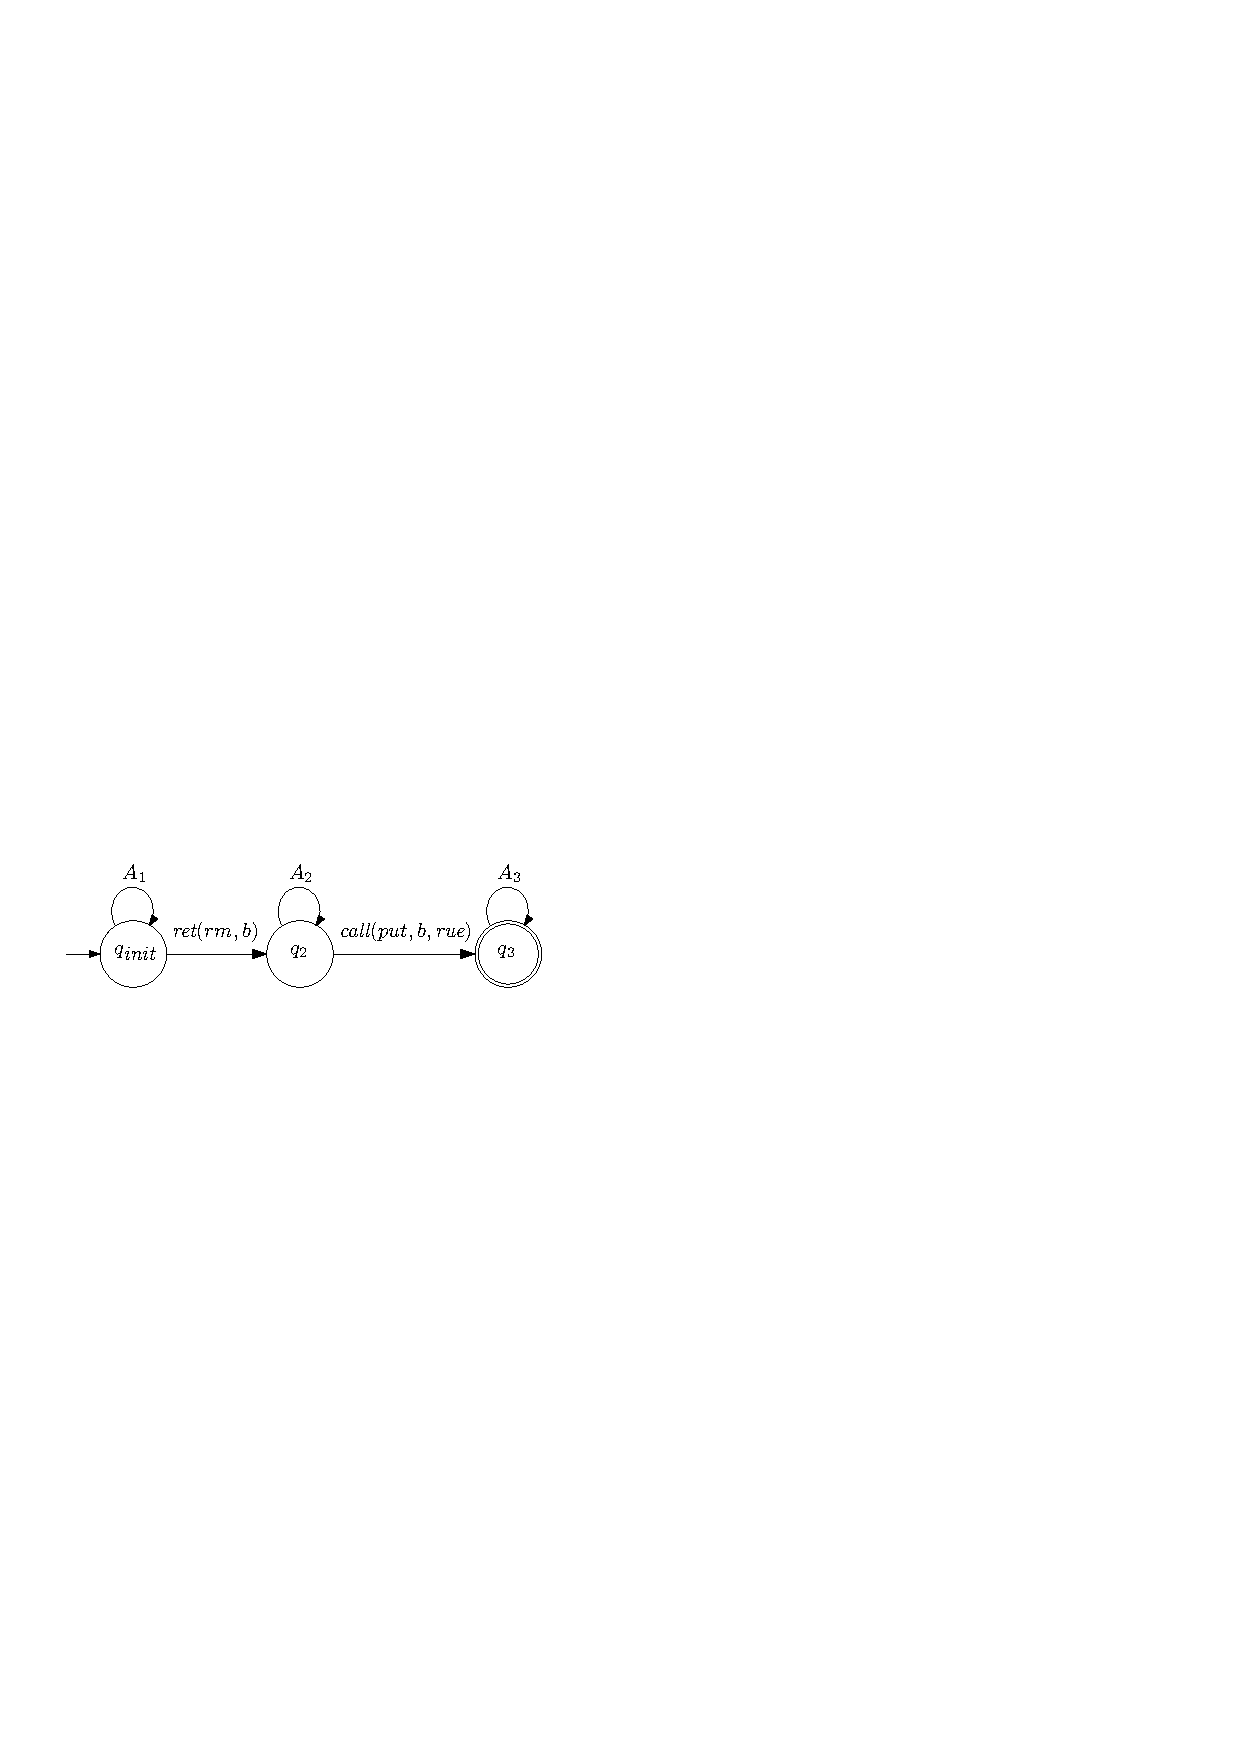
\includegraphics[width=0.6 \textwidth]{figures/PIC_AUTO_FIFO_1.pdf}
%\vspace{-10pt}
  \caption{Automaton $\mathcal{A}_{\textit{SinPri}}^1$}
  \label{fig:automata for FIFO-1 in appendix}
\end{figure}


We generate witness automata $\mathcal{A}_{\textit{SinPri}}^2$ for the second case, and it is shown in \figurename~\ref{fig:automata for FIFO-2}. Here $c_1 = \textit{cal}(\textit{put},a,\textit{anyPri}),\textit{ret}(\textit{put},a), \textit{cal}(\textit{rm},a),\textit{ret}(\textit{rm},a),\textit{cal}(\textit{rm},\textit{empty}),\textit{ret}(\textit{rm},\textit{empty})$, $c_2 = c_1 + \textit{cal}(\textit{rm},b) + \textit{ret}(\textit{rm},b)$.


\begin{figure}[htbp]
  \centering
  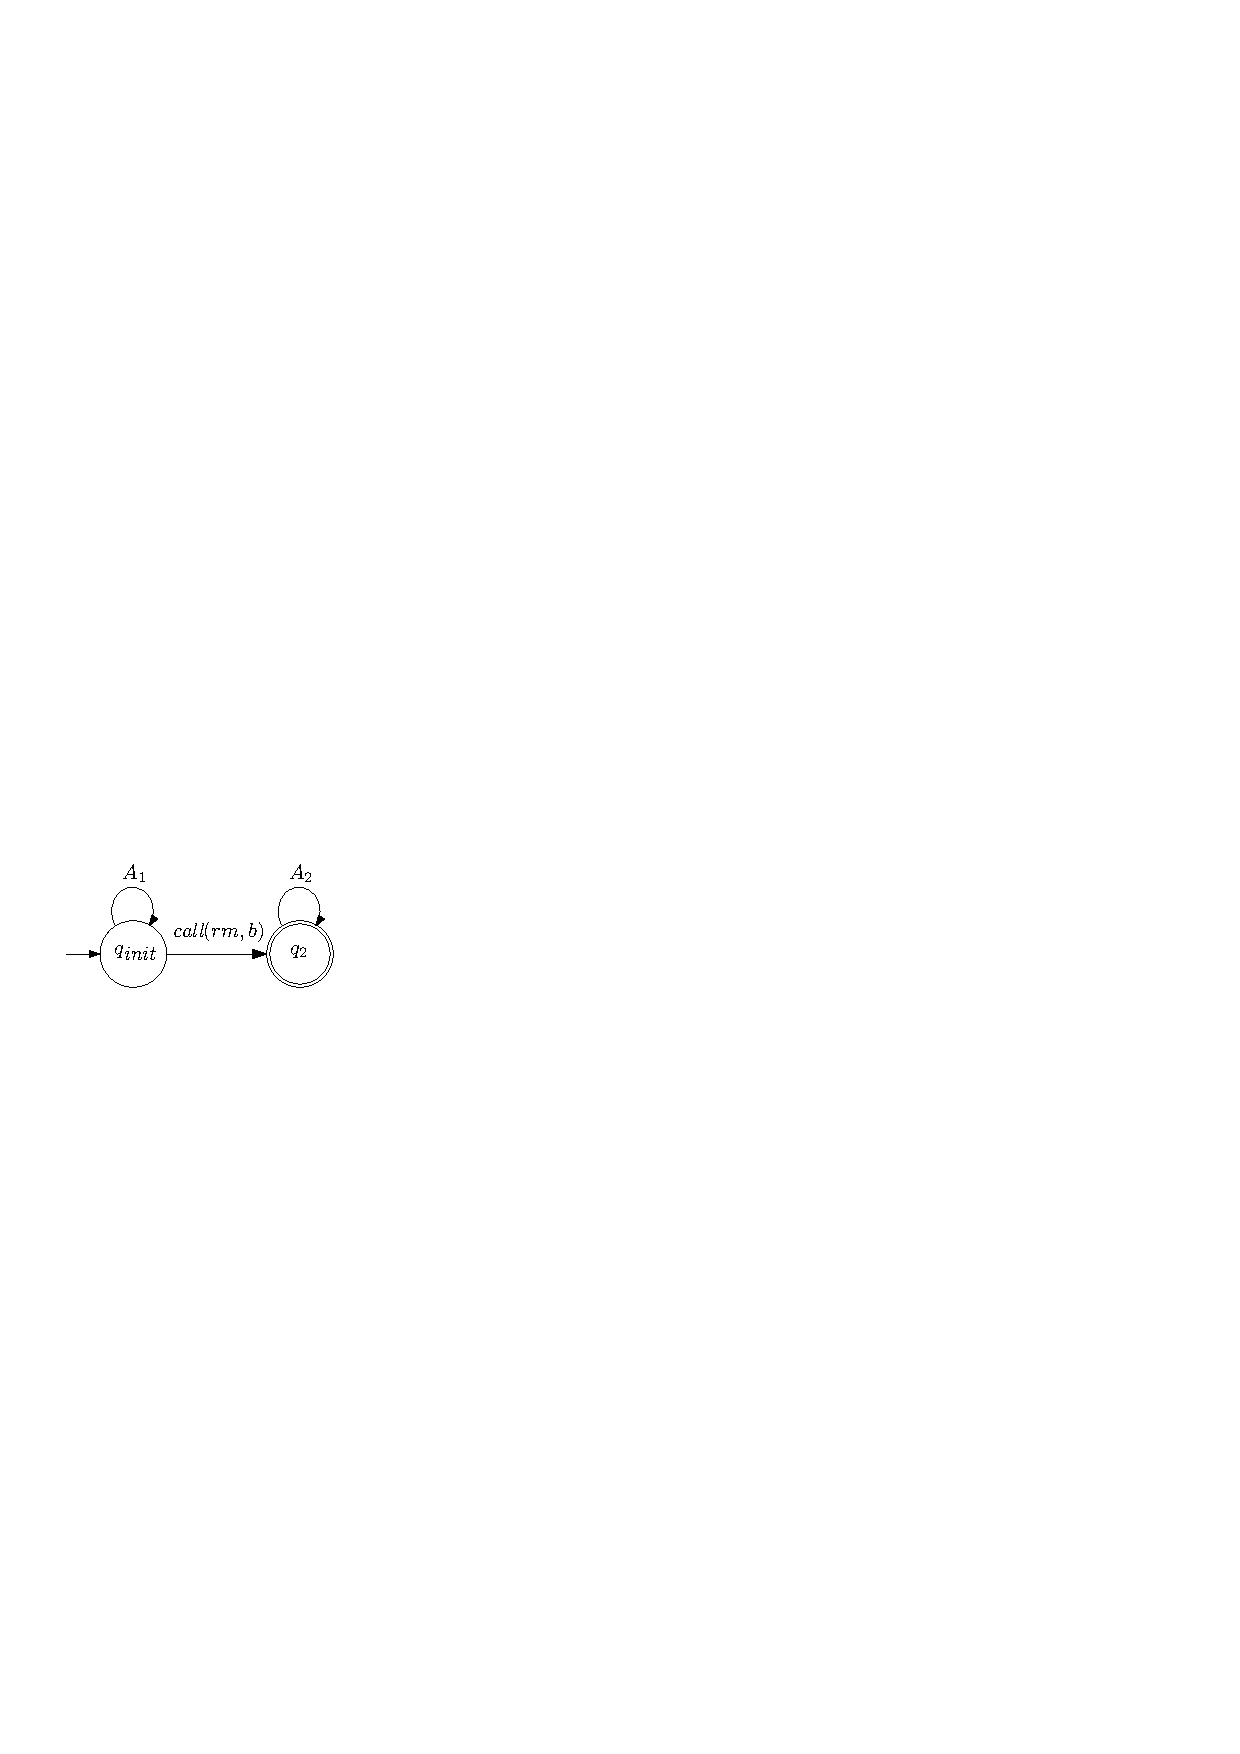
\includegraphics[width=0.3 \textwidth]{figures/PIC_AUTO_FIFO_2.pdf}
%\vspace{-10pt}
  \caption{Automaton $\mathcal{A}_{\textit{SinPri}}^2$}
  \label{fig:automata for FIFO-2}
\end{figure}

We generate witness automata $\mathcal{A}_{\textit{SinPri}}^3$ for the third case, and it is shown in \figurename~\ref{fig:automata for FIFO-3}. Here $c_1 = \textit{cal}(\textit{put},a,\textit{anyPri}),\textit{ret}(\textit{put},a), \textit{cal}(\textit{rm},a),\textit{ret}(\textit{rm},a),\textit{cal}(\textit{rm},\textit{empty}),\textit{ret}(\textit{rm},\textit{empty})$, $c_2 = c_1 + \textit{ret}(\textit{put},b)$, $c_3 = c_2 + \textit{ret}(\textit{rm},b)$, $c_4 = c_3 + \textit{cal}(\textit{rm},b)$, $c_5 = c_1 + \textit{ret}(\textit{rm},b)$, $c_6 = c_5 + \textit{cal}(\textit{rm},b)$.

\begin{figure}[htbp]
  \centering
  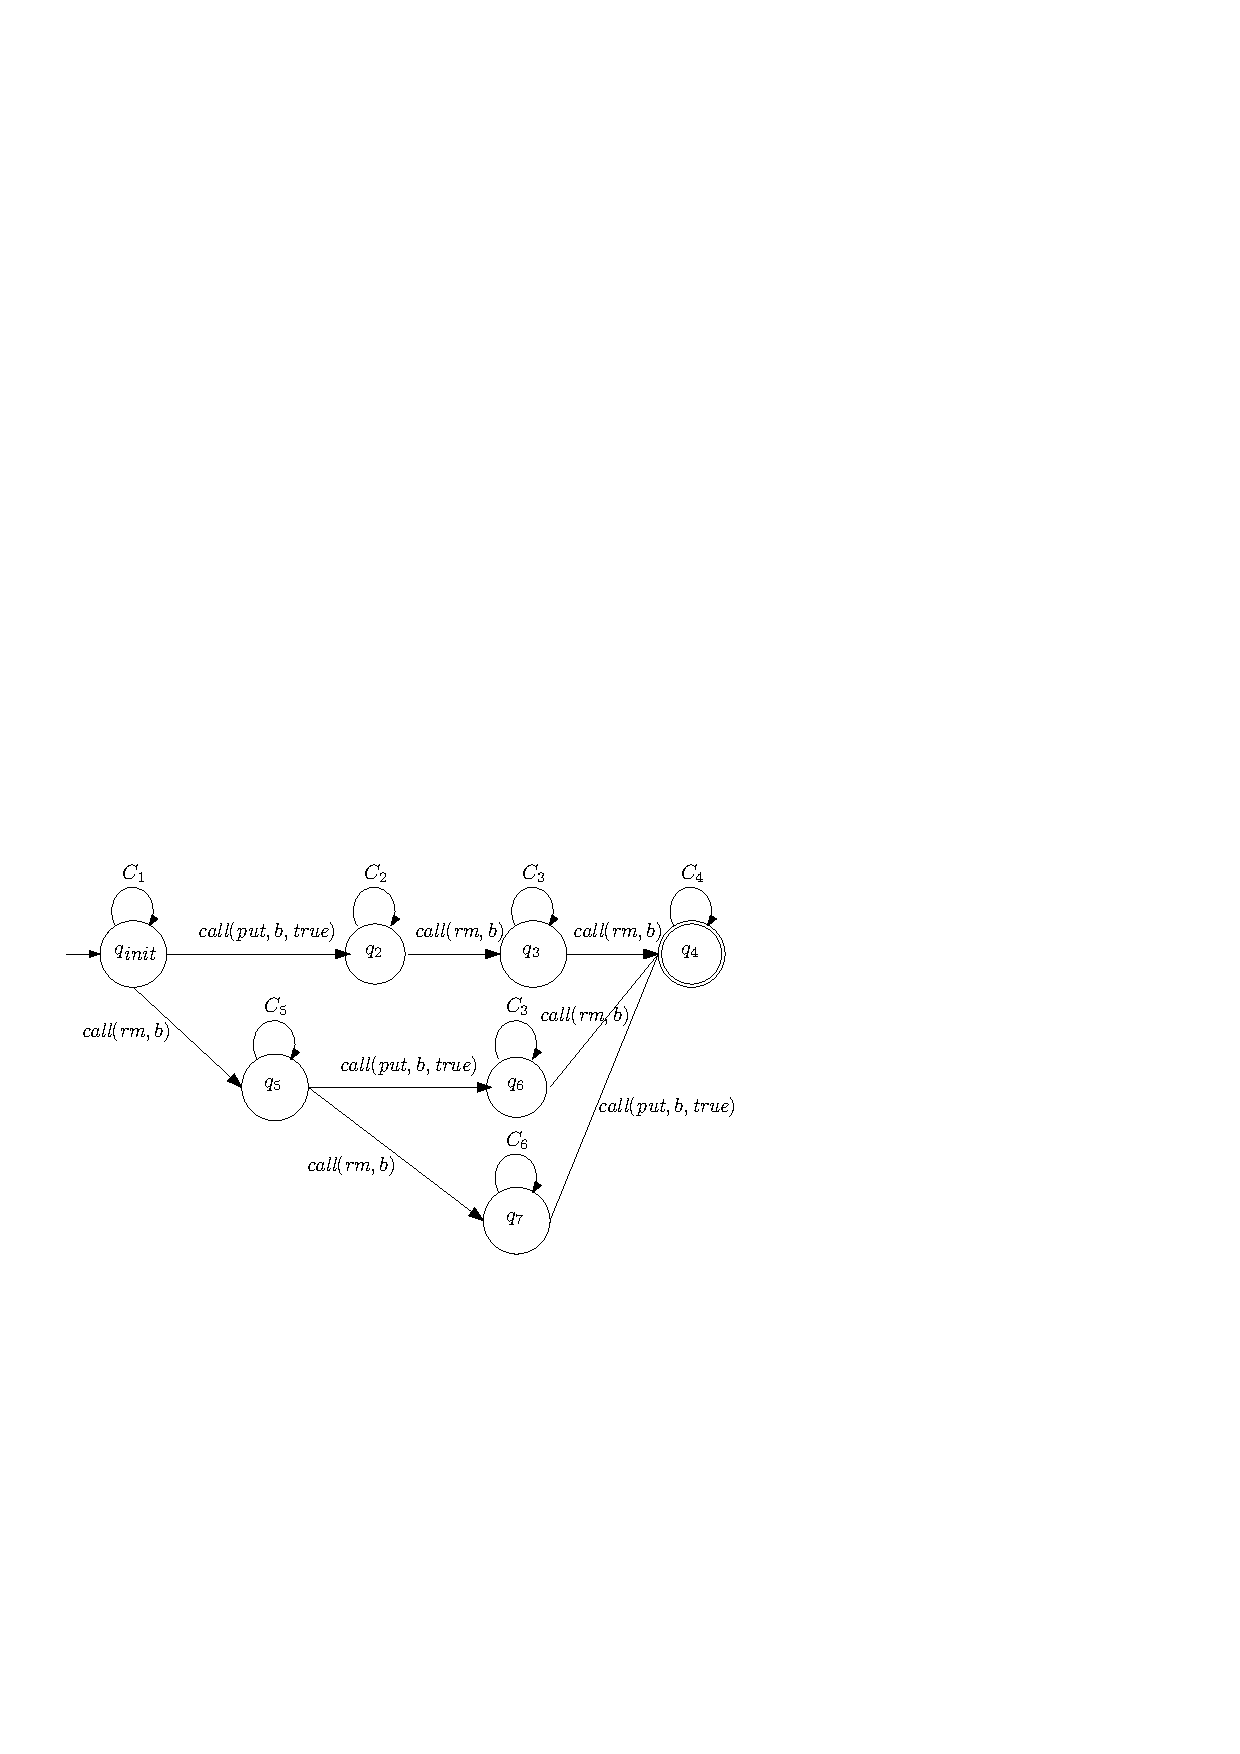
\includegraphics[width=0.7 \textwidth]{figures/PIC_AUTO_FIFO_3.pdf}
%\vspace{-10pt}
  \caption{Automaton $\mathcal{A}_{\textit{SinPri}}^3$}
  \label{fig:automata for FIFO-3}
\end{figure}

We generate witness automata $\mathcal{A}_{\textit{SinPri}}^4$ for the forth case, and it is shown in \figurename~\ref{fig:automata for FIFO-4}. Here $c_1 = c + \textit{cal}(\textit{rm},b)$, and $c_2 = c + \textit{ret}(\textit{put},b) + \textit{cal}(\textit{rm},a) + \textit{ret}(\textit{rm},a)$, where $c = \textit{cal}(\textit{put},d,\textit{anyPri}),\textit{ret}(\textit{put},d), \textit{cal}(\textit{rm},d),\textit{ret}(\textit{rm},d),\textit{cal}(\textit{rm},\textit{empty}),\textit{ret}(\textit{rm},\textit{empty})$.

\begin{figure}[htbp]
  \centering
  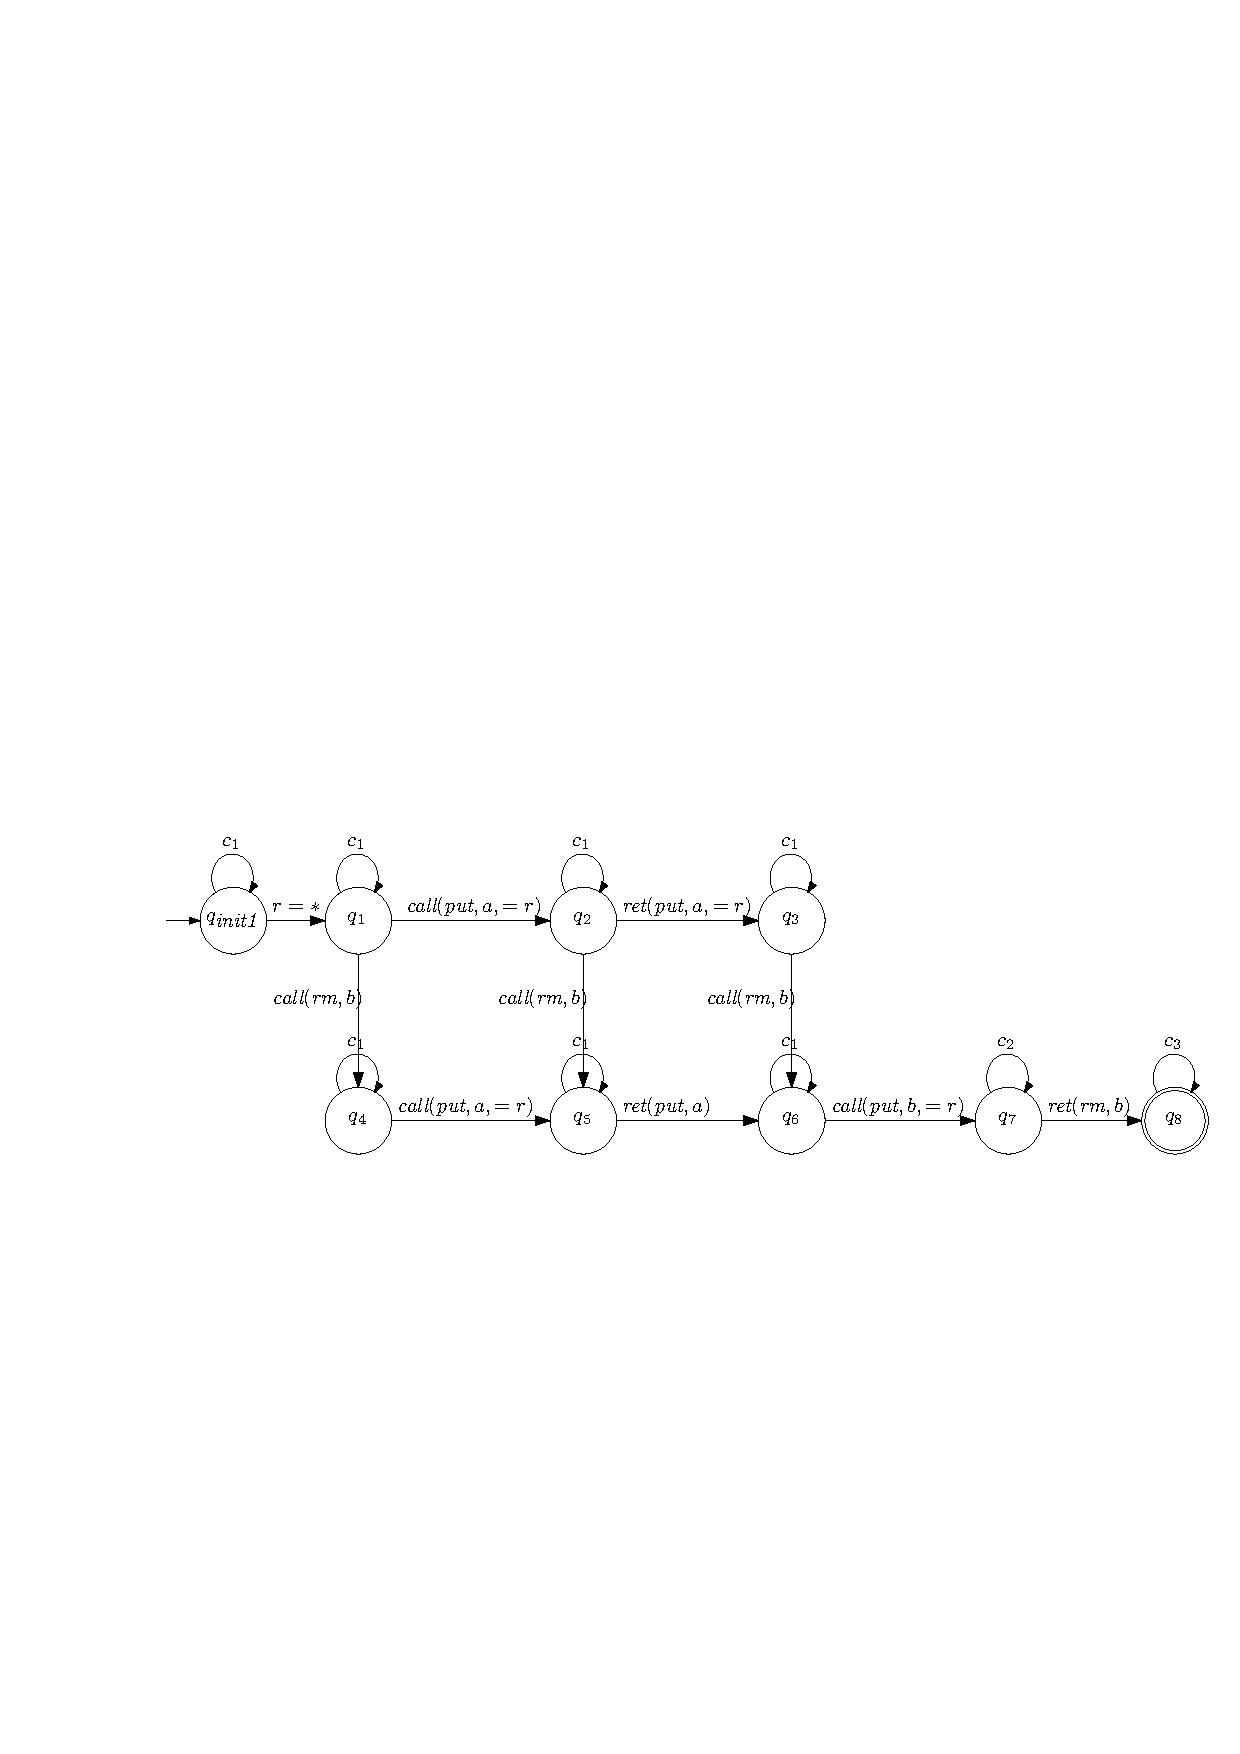
\includegraphics[width=0.9 \textwidth]{figures/PIC_AUTO_FIFO_4.pdf}
%\vspace{-10pt}
  \caption{Automaton $\mathcal{A}_{\textit{SinPri}}^4$}
  \label{fig:automata for FIFO-4}
\end{figure}

Let $\textit{Auts}_{\textit{sinPri}} = \{ \mathcal{A}_{\textit{SinPri}}^1, \mathcal{A}_{\textit{SinPri}}^2, \mathcal{A}_{\textit{SinPri}}^3, \mathcal{A}_{\textit{SinPri}}^4 \}$. Let us prove Lemma \ref{lemma:automata for extended priority queue with single priority}.

\AutoForEPQwithSignlePri*

\begin {proof}

\cite{Bouajjani:2015} states that, given a differentiated queue execution $e$ without $\textit{deq}(\textit{empty})$, $e$ is not linearizable with respect to queue, if one of the following cases holds for some $v_a,v_b$: (1) $\textit{deq}(v_b) <_{hb} \textit{enq}(v_b)$, (2) there are are no $\textit{enq}(v_b)$ and at least one $\textit{deq}(v_b)$, (3) there are are one $\textit{enq}(v_b)$ and more than one $\textit{deq}(v_b)$, and (4) $\textit{enq}(v_a) <_{\textit{hb}} \textit{enq}(v_b)$, and $\textit{deq}(v_b) <_{\textit{hb}} \textit{deq}(v_a)$, or $\textit{deq}(v_a)$ does not exists.

Let us prove the $\textit{only if}$ direction. Assume that there exists execution $e_0 \in \mathcal{I}$ and $e_0$ is accepted by an automaton in $\textit{Auts}_{\textit{sinPri}}$. By data-independence, we can see that there exists a data-differentiated $e \in \mathcal{I}$ and renaming function, such that $e_0=r(e)$. Let $e'$ be obtained from $e$ by first removing $\textit{rm}(\textit{empty})$, and then,

\begin{itemize}
\setlength{\itemsep}{0.5pt}
\item[-] If $e_0$ is accepted by $\mathcal{A}_{\textit{SinPri}}^1$, $\mathcal{A}_{\textit{SinPri}}^2$ or $\mathcal{A}_{\textit{SinPri}}^3$: Then remove all items that are not renamed into $b$ by $r$.

\item[-] If $e_0$ is accepted by $\mathcal{A}_{\textit{SinPri}}^4$: Then remove all items that are not renamed into $a$ or $b$ by $r$.
\end{itemize}

It is obvious that $e' \in \textit{proj}(e)$. It is easy to see that $\textit{transToQueue}(e')$ satisfies one of above conditions, and then $\textit{transToQueue}(e')$ is not linearizable w.r.t queue.

Let us prove the $\textit{if}$ direction. Assume that exists $e \in \mathcal{I}_{\neq}$, $e' \in \textit{proj}(e)$, such that $e'$ is single-priority  without $\textit{rm}(\textit{empty})$, and $\textit{transToQueue}(e')$ does not linearizable to queue. Then we construct a renaming function $r$ as follows:

\begin{itemize}
\setlength{\itemsep}{0.5pt}
\item[-] If this is because case $1$, case $2$ or case $3$: $r$ maps $v_b$ into $b$ and maps all other values into $a$.

\item[-] If this is because case $4$: $r$ maps $v_a$ and $v_b$ into $a$ and $b$, respectively, and maps all other values into $d$.
\end{itemize}

Then it is not hard to see that $r(e) \in \mathcal{I}$ and it is accepted by some automaton in $\textit{Auts}_{\textit{sinPri}}$. This completes the proof of this lemma. \qed
\end {proof}




\subsection{Proofs and Definitions in Subsection \ref{subsec:co-regular of EPQ1Lar}}
\label{sec:appendix proof and definition in section co-regular of EPQ1Lar}

The following lemma states that, from linearization of sub-histories, we can merge them and obtain a linearization (regardless of whether it belongs to sequential specification) of the whole history.

\begin{restatable}{lemma}{MergeTwoLinearization}
\label{lemma:merge two linearization}

Given a history $h$, operation sets $S_1$, $S_2$ and sequences $l_1$ and $l_2$. Let $h_1 = h \vert{S_1}$ and $h_2 = h \vert{S_2}$. Assume that $h_1 \sqsubseteq l_1$, $h_2 \sqsubseteq l_2$, and $S_1 \cup S_2$ contains all operations of $h$. Then, there exists a sequence $l$, such that $h \sqsubseteq l$, $l \vert{S_1} = l_1$ and $l \vert{S_2} = l_2$.
\end{restatable}

\begin {proof}

Given a history $h$ and a operation $o \in S_2$, let $\textit{MB}(o) = \{ o' \vert o' \in S_1$ and $o'$ happens before $o$ in $h \}$, let $\textit{SBI}(o) = \textit{min}\{ i \vert l_1[0,i]$ contains all elements of $\textit{MB}(o) \}$.

Let $l = s_1 \cdot l_2[1] \cdot \ldots \cdot l_2[n] \cdot s_{\textit{n+1}}$ be generated as follows, where $n = \vert l_2 \vert$:

\begin{itemize}
\setlength{\itemsep}{0.5pt}
\item[-] $s_1 = l_1[0, \textit{SBI}(l_2[1])]$,

\item[-] If $s_1 \cdot l_2[1] \cdot \ldots \cdot l_2[i]$ already contains $l_1(\textit{SBI}(l_2[\textit{i+1}]))$, then $s_{\textit{i+1}} = \epsilon$. Otherwise, $s_{\textit{i+1}}$ is a subsequence of $l_1$, which starts from the next of last elements of $s_1 \cdot l_2[1] \cdot \ldots \cdot l_2[i]$ in $l_1$ and ends in $l_1(\textit{SBI}(l_2[\textit{i+1}]))$.
\end{itemize}

It is obvious that $l \vert{S_1} = l_1$ and $l \vert{S_2} = l_2$, and it remains to prove that $h \sqsubseteq l$. We prove this by contradiction. Assume that $h$ is not linearizable with respect to $l$. Then there must be two operations of $h$, such that $o_1 <_{hb} o_2$ in $h$ but $o_2$ before $0_1$ in $l$. Since $l \vert{S_1} = l_1$, $l \vert{S_2} = l_2$, and $h_1 \sqsubseteq l_1$, $h_2 \sqsubseteq l_2$, it is easy to see that it is impossible that $o_1,o_2 \in S_1$ or $o_1,o_2 \in S_2$. There are only two possibilities:

\begin{itemize}
\setlength{\itemsep}{0.5pt}
\item[-] $o_1 \in S_1 \wedge o_2 \in S_2$. Then we can see that $o_2=l_2[i]$ and $o_1 \in s_j$ for some $i < j$. Since $o_1 <_{hb} o_2$, we know that $o_1 \in \textit{SBI}(o_2)$. By the construction of $l$, we know that $o_1$ must be in $s_k$ for some $k \leq i$, contradicts that $o_1 \in s_j$ with $i < j$.

\item[-] $o_1 \in S_2 \wedge o_2 \in S_1$. Then we can see that $o_2 \in s_i$ and $o_1 = l_2[j]$ for some $i \leq j$. It is easy to see that this leads to contradiction when $i = j$. For the case of $i \neq j$, we need to satisfy the following requirements: (1) $o_1$ ($l_2[j]$) does not happen before $l_2[i]$, (2) $l_2[i]$ does not happen before $o_2$, (3) $o_2$ is either overlap or happens before $o' \in \textit{MB}(l_2[i])$, and (4) $o' <_{hb} l_2[i]$. By enumeration we can see that it is impossible that above four conditions be satisfied while $o_1 <_{hb} o_2$.
\end{itemize}

This completes the proof of this lemma. \qed
\end {proof}

With Lemma \ref{lemma:merge two linearization}, we can now prove Lemma \ref{lemma:pri execution is enough}.

\priExecutionIsEnough*
\begin {proof}

We deal with the case of $R = \textit{EPQ}_1^{>}$ , and other cases can be similarly dealt with.

To prove the $\textit{only if}$ direction, given $e \sqsubseteq \textit{MS}(\textit{EPQ}_1^{>})$ and such $\textit{pri}$ and $x$. Since $e \sqsubseteq \textit{MS}(\textit{EPQ}_1^{>})$ with witness $x$, we know that $e \sqsubseteq u \cdot \textit{put}(x,\textit{pri}) \cdot v \cdot \textit{rm}(x) \cdot w$, where $u$, $v$, $w$, $x$ and $\textit{pri}$ satisfy the guard of $\textit{EPQ}_1^{>}$. Let $u'$, $v'$ and $w'$ be obtained from $u$, $v$ and $w$ by erasing all items with priority incomparable with $\textit{pri}$, respectively. It is not hard to see that $u'$, $v'$, $w'$, $x$ and $\textit{pri}$ satisfy the guard of $\textit{EPQ}_1^{>}$, and then $e \sqsubseteq l = u' \cdot \textit{put}(x,\textit{pri}) \cdot v' \cdot \textit{rm}(x) \cdot w' \in \textit{MS}(\textit{EPQ}_1^{>})$.

To prove the $\textit{if}$ direction, given $e' = \textit{pri-Exec}(e)$ and such $x$ and $\textit{pri}$. Since $e' \sqsubseteq \textit{MS}(\textit{EPQ}_1^{>})$ with witness $x$, we know that $e' \sqsubseteq l_1 = u \cdot \textit{put}(x,\textit{pri}) \cdot v \cdot \textit{rm}(x) \cdot w$, where $u$, $v$, $w$, $x$ and $\textit{pri}$ satisfy the guard of $\textit{EPQ}_1^{>}$. Let $O_c$ be the set of operations in $e$ that have priorities comparable with $\textit{pri}$, and Let $O_i$ be the set of operations in $e$ that have priorities incomparable with $\textit{pri}$. It is obvious that $l_1$ is the linearization of $e \vert_{O_c}$. By Lemma \ref{lemma:merge two linearization}, there exists sequence $l$, such that $e \sqsubseteq l$, and $l \vert_{O_c} = l_1$. Then $l = u' \cdot \textit{put}(x,\textit{pri}) \cdot v' \cdot \textit{rm}(x) \cdot w'$, where $u' \vert_{O_c} = u$, $v' \vert_{O_c} = v$ and $w' \vert_{O_c} = w$. Since $\textit{pri}$ is one of maximal priorities in $e$, and the predicates of guards of $\textit{EPQ}_1^{>}$ does not restrict $O_i$, it is easy to see that $l \in \textit{MS}(\textit{EPQ}_1^{>})$ and then $e \sqsubseteq l$ with witness $x$. \qed
\end {proof}


We can see that $\textit{UVSet}_i(e,x) \cap \textit{UVSet}_j(e,x) = \emptyset$ for any $i \neq j$.

The following lemma states that $\textit{UVSet}(e,x)$ contains only matched $\textit{put}$ and $\textit{rm}$.

\begin{restatable}{lemma}{UVSetHasMatchedPutandRm}
\label{lemma:UVSet has matched put and rm}
Given a data-differentiated $\textit{pri}_x$-execution $e$ with $\textit{last}(e) = \textit{EPQ}_1^{>}$. Let $\textit{put}(x,\textit{pri}_x)$ and $\textit{rm}(x)$ be method events of $e$ with maximal priority. Let $G$ be the graph representing the left-right constraint of $\textit{put}(x,\textit{pri}_x)$ and $\textit{rm}(x)$. Assume that $G$ has no cycle going through $x$. Then, $\textit{UVSet}(e,x)$ contains only matched $\textit{put}$ and $\textit{rm}$.
\end{restatable}
\begin {proof}

We prove this lemma by contradiction. Assume that there exists a value, such that $\textit{UVSet}(e,x)$ contains only its $\textit{put}$ and does not contain its $\textit{rm}$. Then we can see that there exists $d_1,\ldots,d_j$. Intuitively, $d_1,\ldots,d_j$ are elements in $\textit{UVSet}_1(e,x), \ldots, \textit{UVSet}_i(e,x)$, respectively. $\textit{UVSet}(e,x)$ contains $\textit{put}(d_j,\_)$ and does not contain $\textit{rm}(d_j)$. And each $d_i$ is the reason of $d_{\textit{i+1}} \in \textit{UVSet}_{\textit{i+1}}(e,x)$. Formally, we require that

\begin{itemize}
\setlength{\itemsep}{0.5pt}
\item[-] For each $1 \leq i \leq j$, method events of $d_i$ belongs to $\textit{UVSet}_i(e,x)$.

\item[-] For each $i \neq j$, $\textit{put}(d_i,\_),\textit{rm}(d_i) \in \textit{UVSet}_i(e,x)$. $\textit{put}(d_j,\_) \in \textit{UVSet}_j(e,x)$, and $e$ does not contain $\textit{rm}(d_j)$.

\item[-] An operation of $d_1$ happens before an operations of $x$. For each $1 < i \leq j$, an operation of $d_i$ happens an operation of $d_{\textit{i-1}}$.

\item[-] For each $k$ and $\textit{ind}$, if $k > \textit{ind+1}$, then no operation of $d_k$ happens before operation of $d_{\textit{ind}}$.
\end{itemize}

According to the definition of $\textit{UVSet}(e,x)$, it is easy to see that such $d_1,\ldots,d_j$ exists. Let us prove the following fact:

\noindent {\bf $\textit{fact}_1$}: Given $1 \leq i < j$, it can not be the case that $\textit{put}(d_i,\_)$ and $\textit{rm}(d_i)$ overlap.

Proof of $\textit{fact}_1$: We prove $\textit{fact}_1$ by contradiction. Assume that for some $i \neq j$, $\textit{put}(d_i,\_)$ and $\textit{rm}(d_i)$ overlap. Since $\textit{put}(d_i,\_), \textit{rm}(d_i) \in \textit{UVSet}_i(h,x)$, we know that an operation $o_i$ of $d_i$ happens before operation $o_{\textit{i-1}}$ of $d_{\textit{i-1}}$. Moreover, since $\textit{put}(d_i,\_)$ and $\textit{rm}(d_i)$ overlap, it is not hard to see that the call action of $\textit{put}(d_i,\_)$ and the call action of $\textit{rm}(d_i)$ is before the call action of $o_{\textit{i-1}}$. Since method events of $d_{\textit{i+1}}$ is in $\textit{UVSet}_{\textit{i+1}}(e,x)$, we know that an operation $o'_{\textit{i+1}}$ of $d_{\textit{i+1}}$ happens before operation $o'_i$ of $d_i$. Then, it is not hard to see that $o'_{\textit{i+1}}$ also happens before $o_{\textit{i-1}}$, which contradicts that for each $k > \textit{ind+1}$, no operation of $d_k$ happens before operation of $d_{\textit{ind}}$.

We already know that an operation of $d_1$ happens before an operation of $x$. By $\textit{fact}_1$, we can ensure that $\textit{put}(d_1,\_)$ happens before an operation of $x$, and then $d_1 \rightarrow x$ in $G$. For each $1 < i \leq j$, we know that an operation $o_i$ of $d_i$ happens before an operation $o_{\textit{i-1}}$ of $d_{\textit{i-1}}$. By $\textit{fact}_1$, we can ensure that $o_i=\textit{put}(d_i,\_)$ and $o_{\textit{i-1}}=\textit{rm}(d_{\textit{i-1}})$, and then $d_i \rightarrow d_{\textit{i-1}}$ in $G$. Since $h$ contains $\textit{put}(d_j,\_)$ and does not contain $\textit{rm}(d_j)$, we know that $x \rightarrow d_j$ in $G$. Then $G$ has a cycle going through $x$, contradicts that $G$ has no cycle going through $x$. \qed
\end {proof}


The following lemma states that $\textit{UVSet}(e,x)$ does not happen before $\textit{rm}(x)$ when the left-right constraint has no cycle going through $x$.

\begin{restatable}{lemma}{RmxDoesNotHappenBeforeUVSetForEPQ1Lar}
\label{lemma:Rmx does not happen before UVSet for EPQ1Lar}

Given a data-differentiated $\textit{pri}_x$-execution $e$ with $\textit{last}(e) = \textit{EPQ}_1^{>}$. Let $\textit{put}(x,\textit{pri}_x)$ and $\textit{rm}(x)$ be method events of $e$ with maximal priority. Let $G$ be the graph representing the left-right constraint of $\textit{put}(x,\textit{pri}_x)$ and $\textit{rm}(x)$. Assume that $G$ has no cycle going through $x$. Then, $\textit{rm}(x)$ does not happen before any operation in $\textit{UVSet}(e,x)$.
\end{restatable}

\begin {proof}

We prove this lemma by induction, and prove that $\textit{rm}(x)$ does not happen before any operation in $\textit{UVSet}_1(e,x)$, in $\textit{UVSet}_2(e,x)$, $\ldots$. Note that, by Lemma \ref{lemma:UVSet has matched put and rm}, $\textit{UVSet}(e,x)$ contains only matched $\textit{put}$ and $\textit{rm}$, and it is easy to see that for each $i$, $\textit{UVSet}_i(e,x)$ contains only matched $\textit{put}$ and $\textit{rm}$.

\noindent (1) Let us prove that $\textit{rm}(x)$ does not happen before any operation in $\textit{UVSet}_1(e,x)$ by contradiction. Assume that $\textit{rm}(x) <_{hb} o$, where $o \in \textit{UVSet}_1(e,x)$ is an operation of item $d$. %(according to the definition of $\textit{UVSet}_1(h,x)$, the priority of $d$ does not equals $\textit{pri}_x$).

We use a triple $(t_1,t_2,t_3)$ to represent related information. $t_1,t_2,t_3$ are chosen from $\{ \textit{put},\textit{rm} \}$. $t_1$ represents whether $o$ is a $\textit{put}$ method event or a $\textit{rm}$ method event. $t_2$ and $t_3$ is used for the reason of $o \in \textit{UVSet}_1(e,x)$: $o \in \textit{UVSet}_1(e,x)$, since an operation (of kind $t_2$) of $d$ happens before an operation (of kind $t_3$) of $x$. Let us consider all the possible cases of $(t_1,t_2,t_3)$:

\begin{itemize}
\setlength{\itemsep}{0.5pt}
\item[-] $(\textit{put},\textit{put},\textit{put})$: Then $\textit{rm}(x) <_{hb} \textit{put}(d,\_) <_{hb} \textit{put}(x,\textit{pri}_x)$, contradicts that $\textit{rm}(x)$ does not happen before $\textit{put}(x,\textit{pri}_x)$.

\item[-] $(\textit{put},\textit{put},\textit{rm})$: Then $\textit{rm}(x) <_{hb} \textit{put}(d,\_) <_{hb} \textit{rm}(x)$, contradicts that $\textit{rm}(x)$ does not happen before $\textit{rm}(x)$.

\item[-] $(\textit{put},\textit{rm},\textit{put})$: Then $( \textit{rm}(x) <_{hb} \textit{put}(d,\_) ) \wedge ( \textit{rm}(d) <_{hb} \textit{put}(x,\textit{pri}_x) )$. By interval order, we know that $( \textit{rm}(x) <_{hb} \textit{put}(x,\textit{pri}_x) ) \vee ( \textit{rm}(d) <_{hb} \textit{put}(d,\_) )$, which is impossible.

\item[-] $(\textit{put},\textit{rm},\textit{rm})$: Then $( \textit{rm}(x) <_{hb} \textit{put}(d,\_) ) \wedge ( \textit{rm}(d) <_{hb} \textit{rm}(x) )$. We can see that $\textit{rm}(d) <_{hb} \textit{rm}(x) <_{hb} \textit{put}(d,\_)$, which contradicts that $\textit{rm}(d)$ does not happen before $\textit{put}(d,\_)$.

\item[-] $(\textit{rm},\textit{put},\textit{put})$: Then $( \textit{rm}(x) <_{hb} \textit{rm}(d) ) \wedge ( \textit{put}(d,\_) <_{hb} \textit{put}(x,\textit{pri}_x) )$. We can see that $x$ and $d$ has circle in $G$, contradicts that $G$ has no cycle going through $x$.

\item[-] $(\textit{rm},\textit{put},\textit{rm})$: Then $( \textit{rm}(x) <_{hb} \textit{rm}(d) ) \wedge ( \textit{put}(d,\_) <_{hb} \textit{rm}(x) )$. We can see that $x$ and $d$ has circle in $G$, contradicts that $G$ has no cycle going through $x$.

\item[-] $(\textit{rm},\textit{rm},\textit{put})$: Then $\textit{rm}(x) <_{hb} \textit{rm}(d) <_{hb} \textit{put}(x,\textit{pri}_x)$, contradicts that $\textit{rm}(x)$ does not happen before $\textit{put}(x,\textit{pri}_x)$.

\item[-] $(\textit{rm},\textit{rm},\textit{rm})$: Then $\textit{rm}(x) <_{hb} \textit{rm}(d) <_{hb} \textit{rm}(x)$, contradicts that $\textit{rm}(x)$ does not happen before $\textit{rm}(x)$.
\end{itemize}

This completes the proof for $\textit{UVSet}_1(e,x)$.

\noindent (2) Assume we already prove that for some $j \geq 1$, $\textit{rm}(x)$ does not happen before any operation in $\textit{UVSet}_1(e,x) \cup \ldots \cup \textit{UVSet}_j(e,x)$. Let us prove that $\textit{rm}(x)$ does not happen before any operation in $\textit{UVSet}_{\textit{j+1}}(e,x)$ by contradiction. Assume that $\textit{rm}(x) <_{hb} o$, where $o \in \textit{UVSet}_{\textit{j+1}}(e,x)$ is an operation of item $d_{\textit{j+1}}$. We use a triple $(t_1,t_2,t_3)$ to represent related information. $t_1,t_2,t_3$ are chosen from $\{ \textit{put},\textit{rm} \}$. $t_1$ represents whether $o$ is a $\textit{put}$ method event or a $\textit{rm}$ method event. $t_2$ and $t_3$ is used for the reason of $o \in \textit{UVSet}_{\textit{j+1}}(e,x)$: $o \in \textit{UVSet}_{\textit{j+1}}(e,x)$, since an operation (of kind $t_2$) of $d_{\textit{j+1}}$ happens before an operation (of kind $t_3$) of $d_j$, where $\textit{put}(d_j,\_), \textit{rm}(d_j) \in \textit{UVSet}_j(e,x)$. Let us consider all the possible cases of $(t_1,t_2,t_3)$:

\begin{itemize}
\setlength{\itemsep}{0.5pt}
\item[-] $(\textit{put},\textit{put},\textit{put})$: Then $\textit{rm}(x) <_{hb} \textit{put}(d_{\textit{j+1}},\_) <_{hb} \textit{put}(d_j,\_)$. We can see that $( \textit{rm}(x) <_{hb} \textit{put}(d_j,\_) ) \wedge ( \textit{put}(d_j,\_) \in \textit{UVSet}_j(e,x) )$, which contradicts that $\textit{rm}(x)$ does not happen before any operation in $\textit{UVSet}_1(e,x) \cup \ldots \cup \textit{UVSet}_j(e,x)$.

\item[-] $(\textit{put},\textit{put},\textit{rm})$: Then $\textit{rm}(x) <_{hb} \textit{put}(d_{\textit{j+1}},\_) <_{hb} \textit{rm}(d_j,\_)$. We can see that $( \textit{rm}(x) <_{hb} \textit{rm}(d_j,\_) ) \wedge ( \textit{rm}(d_j) \in \textit{UVSet}_j(e,x) )$, which contradicts that $\textit{rm}(x)$ does not happen before any operation in $\textit{UVSet}_1(e,x) \cup \ldots \cup \textit{UVSet}_j(e,x)$.

\item[-] $(\textit{put},\textit{rm},\textit{put})$: Then $( \textit{rm}(x) <_{hb} \textit{put}(d_{\textit{j+1}},\_) ) \wedge ( \textit{rm}(d_{\textit{j+1}}) <_{hb} \textit{put}(d_j,\_) )$. By interval order, we know that $( \textit{rm}(x) <_{hb} \textit{put}(d_j,\_) ) \vee ( \textit{rm}(d_{\textit{j+1}}) <_{hb} \textit{put}(d_{\textit{j+1}},\_) )$, which is impossible.

\item[-] $(\textit{put},\textit{rm},\textit{rm})$: Then $( \textit{rm}(x) <_{hb} \textit{put}(d_{\textit{j+1}},\_) ) \wedge ( \textit{rm}(d_{\textit{j+1}}) <_{hb} \textit{rm}(d_j) )$. By interval order, we know that $( \textit{rm}(x) <_{hb} \textit{rm}(d_j) ) \vee ( \textit{rm}(d_{\textit{j+1}}) <_{hb} \textit{put}(d_{\textit{j+1}},\_) )$, which is impossible.

\item[-] $(\textit{rm},\textit{put},\textit{put})$: Then $( \textit{rm}(x) <_{hb} \textit{rm}(d_{\textit{j+1}}) ) \wedge ( \textit{put}(d_{\textit{j+1}},\_) <_{hb} \textit{put}(d_j,\_) )$. Let us consider the reason of $\textit{put}(d_j,\_), \textit{rm}(d_j) \in \textit{UVSet}_j(e,x)$:
    \begin{itemize}
    \setlength{\itemsep}{0.5pt}
    \item[-] If $( j > 1 ) \wedge ( \textit{put}(d_j,\_) <_{hb} o'' )$, where $o''$ is an operation of item $d_{\textit{j-1}}$ and $\textit{put}(d_{\textit{j-1}},\_), \textit{rm}(d_{\textit{j-1}}) \in \textit{UVSet}_{\textit{j-1}}(e,x)$: Then since $( \textit{put}(d_{\textit{j+1}},\_) <_{hb} \textit{put}(d_j,\_) ) \wedge ( \textit{put}(d_j,\_) <_{hb} o'' )$, we can see that $\textit{put}(d_{\textit{j+1}},\_) <_{hb} o''$, and then operations of $d_{\textit{j+1}}$ is in $\textit{UVSet}_j(e,x)$, contradicts that operations of $d_{\textit{j+1}}$ is in $\textit{UVSet}_{\textit{j+1}}(e,x)$.

    \item[-] If $( j = 1 ) \wedge ( \textit{put}(d_j,\_) <_{hb} o'' )$, where $o''$ is an operation of $x$: Similar to above case.

    \item[-] If $( j > 1 ) \wedge ( \textit{rm}(d_j) <_{hb} o'' )$, where $o''$ is an operation of item $d_{\textit{j-1}}$ and $\textit{put}(d_{\textit{j-1}},\_), \textit{rm}(d_{\textit{j-1}}) \in \textit{UVSet}_{\textit{j-1}}(e,x)$: Then since $( \textit{put}(d_{\textit{j+1}},\_) <_{hb} \textit{put}(d_j,\_) ) \wedge ( \textit{rm}(d_j) <_{hb} o'' )$, we can see that $( \textit{put}(d_{\textit{j+1}},\_) <_{hb} o'' ) \vee ( \textit{rm}(d_j) <_{hb} \textit{put}(d_j,\_) )$, which is impossible.

    \item[-] If $( j > 1 ) \wedge ( \textit{rm}(d_j) <_{hb} o'' )$, where $o''$ is an operation of $x$: Similar to above case.
    \end{itemize}

\item[-] $(\textit{rm},\textit{put},\textit{rm})$: Let $T_{\textit{ind}}$ be the set of sentences $\{ \textit{rm}(x) <_{hb} \textit{rm}(d_{\textit{j+1}}), \textit{put}(d_{\textit{j+1}},\_) <_{hb} \textit{rm}(d_j),\ldots, \textit{put}(d_{\textit{ind+1}},\_) <_{hb} \textit{rm}(d_{\textit{ind}}) \}$. Here each $d_i$ is a item of some operation in $\textit{UVSet}_i(e,x)$. Let us prove that from $T_j$ we can obtain contradiction by induction:

    {\bf Base case $1$}: From $T_1$ we can obtain contradiction.

    Let us prove base case $1$:

    \begin{itemize}
    \setlength{\itemsep}{0.5pt}
    \item[-] If $\textit{put}(d_1,\_)$ happens $o$, and $o$ is an operation of $x$. Then there is a cycle $x \rightarrow d_{\textit{j+1}} \rightarrow \ldots \rightarrow d_1 \rightarrow x$ in $G$, contradicts that $G$ has no cycle going through $x$.

    \item[-] If $\textit{rm}(d_1)$ happens before $o$, and $o$ is an operation of $x$. Then since $\textit{put}(d_2,\_) <_{hb} \textit{rm}(d_1)$ and $\textit{rm}(d_1) <_{hb} o$, we can see that $\textit{put}(d_2,\_) <_{hb} o$, and then $\textit{put}(d_2,\_) \in \textit{UVSet}_1(e,x)$, contradicts that $\textit{put}(d_2,\_) \in \textit{UVSet}_2(e,x)$.
    \end{itemize}

    {\bf Base case $2$}: From $T_2$ we can obtain contradiction.

    Let us prove base case $2$: If $\textit{rm}(d_2) <_{hb} o$, and $o$ is an operation of $d_1$, then since $( \textit{put}(d_3,\_) <_{hb} \textit{rm}(d_2) ) \wedge ( \textit{rm}(d_2) <_{hb} o )$, we know that $\textit{put}(d_3,\_) <_{hb} o$. This implies that $\textit{put}(d_3,\_) \in \textit{UVSet}_2(e,x)$, contradicts that $\textit{rm}(d_3,\_) \in \textit{UVSet}_3(e,x)$. Therefore, it is only possible that $\textit{put}(d_2,\_)$ happens before an operation of $d_1$.

    \begin{itemize}
    \setlength{\itemsep}{0.5pt}
    \item[-] If $\textit{put}(d_2,\_) <_{hb} \textit{put}(d_1,\_)$ and $\textit{put}(d_1,\_)$ happens before operations of $x$, then we know that $\textit{put}(d_2,\_)$ happens before operation of $x$, which is impossible.

    \item[-] If $\textit{put}(d_2,\_) <_{hb} \textit{put}(d_1,\_)$ and $\textit{rm}(d_1)$ happens before operations of $x$, then by interval order, we know that $\textit{put}(d_2,\_)$ happens before operation of $x$, or $\textit{rm}(d_1) <_{hb} \textit{put}(d_1,\_)$, which is impossible.

    \item[-] If $\textit{put}(d_2,\_) <_{hb} \textit{rm}(d_1)$ and $\textit{put}(d_1,\_)$ happens before operations of $x$, then $x \rightarrow d_{\textit{j+1}} \rightarrow \ldots \rightarrow d_1 \rightarrow x$ in $G$, contradicts that $G$ has no cycle going through $x$.

    \item[-] If $\textit{put}(d_2,\_) <_{hb} \textit{rm}(d_1)$ and $\textit{rm}(d_1)$ happens before operations of $x$, then we know that $\textit{put}(d_2,\_)$ happens before operation of $x$, which is impossible.
    \end{itemize}

    {\bf induction step}: Given $\textit{ind} \geq 3$, if from $T_{\textit{ind-1}}$ we can obtain contradiction, then from $T_{\textit{ind}}$ we can also contain contradiction.


    Prove of the induction step: Similarly as base case $2$, we can prove that it is only possible that $\textit{put}(d_{\textit{ind}},\_)$ happens before operations of $d_{\textit{ind-1}}$.

    \begin{itemize}
    \setlength{\itemsep}{0.5pt}
    \item[-] If $\textit{put}(d_{\textit{ind}},\_) <_{hb} \textit{put}(d_{\textit{ind-1}},\_)$ and $\textit{put}(d_{\textit{ind-1}},\_)$ happens before operations of $d_{\textit{ind-2}}$, then we know that $\textit{put}(d_{\textit{ind}})$ happens before operation of $d_{\textit{ind-2}}$, which is impossible.

    \item[-] If $\textit{put}(d_{\textit{ind}},\_) <_{hb} \textit{put}(d_{\textit{ind-1}},\_)$ and $\textit{rm}(d_{\textit{ind-1}})$ happens before operations of $d_{\textit{ind-2}}$, then by interval order, we know that $\textit{put}(d_{\textit{ind}},\_)$ happens before operation of $d_{\textit{ind-2}}$, or $\textit{rm}(d_{\textit{ind-1}}) <_{hb} \textit{put}(d_{\textit{ind-1}},\_)$, which is impossible.

    \item[-] If $\textit{put}(d_{\textit{ind}},\_) <_{hb} \textit{rm}(d_{\textit{ind-1}})$, then we obtain $T_{\textit{ind-1}}$, which already contain contradiction.
    \end{itemize}

    By base case $1$, base case $2$ and the induction step, it is easy to see that for each $i$, $T_i$ contains contradiction. Therefore, $T_j$, the case of $(\textit{rm},\textit{put},\textit{rm})$, contains contradiction.

\item[-] $(\textit{rm},\textit{rm},\textit{put})$: Then $( \textit{rm}(x) <_{hb} \textit{rm}(d_{\textit{j+1}}) ) \wedge ( \textit{rm}(d_{\textit{j+1}}) <_{hb} \textit{put}(d_j,\_) )$. We can see that $( \textit{rm}(x) <_{hb} \textit{put}(d_j,\_) ) \wedge ( \textit{put}(d_j,\_) \in \textit{UVSet}_j(e,x) )$, which contradicts that $\textit{rm}(x)$ does not happen before any operation in $\textit{UVSet}_1(e,x) \cup \ldots \cup \textit{UVSet}_j(e,x)$.

\item[-] $(\textit{rm},\textit{rm},\textit{rm})$: Then $( \textit{rm}(x) <_{hb} \textit{rm}(d_{\textit{j+1}}) ) \wedge ( \textit{rm}(d_{\textit{j+1}}) <_{hb} \textit{rm}(d_j) )$. We can see that $( \textit{rm}(x) <_{hb} \textit{rm}(d_j) ) \wedge ( \textit{rm}(d_j) \in \textit{UVSet}_j(e,x) )$, which contradicts that $\textit{rm}(x)$ does not happen before any operation in $\textit{UVSet}_1(e,x) \cup \ldots \cup \textit{UVSet}_j(e,x)$.
\end{itemize}

This completes the proof for $\textit{UVSet}_{\textit{j+1}}(e,x)$. Therefore, $\textit{rm}(x)$ does not happen before any operation in $\textit{UVSet}(e,x) = \textit{UVSet}_1(e,x) \cup \textit{UVSet}_2(e,x) \cup \ldots$. \qed
\end {proof}

With Lemma \ref{lemma:UVSet has matched put and rm} and Lemma \ref{lemma:Rmx does not happen before UVSet for EPQ1Lar}, we can now prove Lemma \ref{lemma:Lin Equals Constraint for EPQ1Lar}.

\LinEqualsConstraintforEPQOneLar*

\begin {proof}

To prove the $\textit{only if}$ direction, assume that $e \sqsubseteq \textit{MS}(\textit{EPQ}_1^{>})$. Let $u$, $v$ and $w$ be the sequences of method events in $\textit{EPQ}_1^{>}$, and let $U$, $V$ and $W$ be the set of method events of $u$, $v$ and $w$, respectively. Assume by contradiction that, there is a cycle $d_1 \rightarrow d_2 \rightarrow \ldots \rightarrow d_m \rightarrow x \rightarrow d_1$ in $G$. It is obvious that the priority of each $d_i$ is smaller than $\textit{pri}_x$. Then our proof proceeds as follows:

According to the definition of left-right constraint, there are two possibilities. The first possibility is that, $\textit{rm}(x)$ happens before $\textit{rm}(d_1)$. It is obvious that $\textit{rm}(d_1) \in W$, and then since $U \cup V$ contains matched $\textit{put}$ and $\textit{rm}$, we can see that $\textit{put}(d_1),\textit{rm}(d_1) \in W$. Then,

\begin{itemize}
\setlength{\itemsep}{0.5pt}
\item[-] Since $d_1 \rightarrow d_2$, by definition of $G$, we know that $\textit{put}(d_1)$ happens before $\textit{rm}(d_2)$. Since $\textit{put}(d_1) \in W$ and $U \cup V$ contains matched $\textit{put}$ and $\textit{rm}$, we know that $\textit{put}(d_2),\textit{rm}(d_2) \in W$. Similarly, for each $1 \leq i \leq m$, we know that $\textit{put}(d_i),\textit{rm}(d_i) \in W$.

\item[-] Since $d_m \rightarrow x$,
    \begin{itemize}
    \setlength{\itemsep}{0.5pt}
    \item[-] if $\textit{put}(d_m)$ happens before $\textit{put}(x)$, then we can see that $\textit{put}(d_m) \in U$, which contradicts that $\textit{put}(d_m) \in W$.

    \item[-] if $\textit{put}(d_m)$ happens before $\textit{rm}(x)$, then we can see that $\textit{put}(d_m) \in U \cup V$, which contradicts that $\textit{put}(d_m) \in W$.
    \end{itemize}
\end{itemize}

The second possibility is that, $e$ contains one $\textit{put}(d_1,\_)$ and no $\textit{rm}(d_1)$. Note that for each $j > 1$, $e$ contains $\textit{put}(d_j,\_)$ and $\textit{rm}(d_j)$. Since $d_m \rightarrow x$, is is obvious that $\textit{put}(d_m) \in U \cup V$. Since $U \cup V$ contains matched $\textit{put}$ and $\textit{rm}$, we know that $\textit{put}(d_m),\textit{rm}(d_m) \in U \cup V$. Then, since $d_{\textit{m-1}} \rightarrow d_m$, by definition of $G$, we know that $\textit{put}(d_{\textit{m-1}})$ happens before $\textit{rm}(d_m)$. Since $\textit{rm}(d_m) \in U \cup V$ and $U \cup V$ contains matched $\textit{put}$ and $\textit{rm}$, we know that $\textit{put}(d_{\textit{m-1}}),\textit{rm}(d_{\textit{m-1}}) \in U \cup V$. Similarly, for each $1 < i \leq m$, we know that $\textit{put}(d_i),\textit{rm}(d_i) \in U \cup V$, and also $\textit{put}(d_1)\in U \cup V$. However, there is one $\textit{put}(d_1,\_)$ and no $\textit{rm}(d_1)$ in $e$, contradicts that $U \cup V$ contains matched $\textit{put}$ and $\textit{rm}$.

This completes the proof of the $\textit{only if}$ direction.

To prove the $\textit{if}$ direction, assume that $G$ has no cycle going through $x$. Let $E_u$ be the set of operations that happen before $\textit{put}(x)$ in $e$. It is easy to see that $E_u \subseteq \textit{UVSet}(e,x)$. Let $E_v = \textit{UVSet}(e,x) \setminus E_u$. Let $E_e$ be the set of operations of $e$, and let $E_w = E_e \setminus \textit{UVSet}(e,x)$.

By Lemma \ref{lemma:UVSet has matched put and rm}, we can see that $E_u \cup E_v$ contains matched $\textit{put}$ and $\textit{rm}$ operations. It remains to prove that for $E_u$, $\{ \textit{put}(x,\textit{pri}_x) \}$, $E_v$, $\{ \textit{rm}(x) \}$, $E_w$, no elements of the latter set happens before elements of the former set. We prove this by showing that all the following cases are impossible:

\begin{itemize}
\setlength{\itemsep}{0.5pt}
\item[-] Case $1$: Some operation $o_w \in E_w$ happens before $\textit{rm}(x)$. Then we know that $o_w \in \textit{UVSet}(e,x) = E_u \cup E_v$, which contradicts that $o_w \in E_w$.

\item[-] Case $2$: Some operation $o_w \in E_w$ happens before some operation $o_{\textit{uv}} \in E_u \cup E_v$. Then we know that $o_w \in \textit{UVSet}(e,x) = E_u \cup E_v$, which contradicts that $o_w \in E_w$.

\item[-] Case $3$: Some operation $o_w \in E_w$ happens before $\textit{put}(x)$. Then we know that $o_w \in \textit{UVSet}(e,x) = E_u \cup E_v$, which contradicts that $o_w \in E_w$.

\item[-] Case $4$: $\textit{rm}(x)$ happens before some $o_{\textit{uv}} \in \textit{UVSet}(e,x) = E_u \cup E_v$. By Lemma \ref{lemma:Rmx does not happen before UVSet for EPQ1Lar} we know that this is impossible.

\item[-] Case $5$: $\textit{rm}(x)$ happens before $\textit{put}(x)$. This contradicts that each single-priority projection satisfy the FIFO property.

\item[-] Case $6$: Some operation $o_v \in E_v$ happens before $\textit{put}(x)$. Then we know that $o_v \in E_u$, which contradicts that $o_v \in E_v$.

\item[-] Case $7$: Some operation $o_v \in E_v$ happens before some operation $o_u \in E_u$. Then we know that $o_v \in E_u$, which contradicts that $o_v \in E_v$.

\item[-] Case $8$: $\textit{put}(x)$ happens before some operation $o_u \in E_u$. This is impossible.
\end{itemize}

This completes the proof of the $\textit{if}$ direction.

\qed
\end {proof}


Let us begin to represent witness automata that is used for capture the existence of a data-differentiated execution $e$, $e$ has a $\_$-projection $e'$, $\textit{last}(e') = \textit{PQ}_1^{>}$, and there exists a cycle going through the item with maximal priority in $e'$. By data-independence, we can obtain $e_r$ from $e$ by renaming function, which maps such item to be $b$, maps items that cover it to be $a$, and maps other items into $d$. There are four possible enumeration of call and return actions of $\textit{put}(b)$ and $\textit{rm}(b)$. For each of them, we generate a witness automaton.

For the case when $e_r \vert_{b} = \textit{cal}(\textit{put},b,p) \cdot \textit{ret}(\textit{put}) \cdot \textit{cal}(\textit{rm}) \cdot \textit{ret}(\textit{rm},b)$, we generate witness automaton $\mathcal{A}_{\textit{l-lar}}^1$, as shown in \figurename~\ref{fig:automata APQ1Lar-1}. Here $c_1 = c + \textit{ret}(\textit{rm},a)$, $c_2 = c + \textit{cal}(\textit{put},a,\textit{les}_p)$, $c_3 = c_2 + \textit{ret}(\textit{rm},a)$, where $c = \textit{cal}(\textit{put},d,\textit{anyPri}),\textit{ret}(\textit{put},d), \textit{cal}(\textit{rm},d)$, $\textit{ret}(\textit{rm},d),\textit{cal}(\textit{rm},\textit{empty}),\textit{ret}(\textit{rm},\textit{empty})$. The differentiated branch in $\mathcal{A}_{\textit{l-lar}}^1$ comes from the positions of the first $\textit{ret}(\textit{put},a)$.

\begin{figure}[htbp]
  \centering
  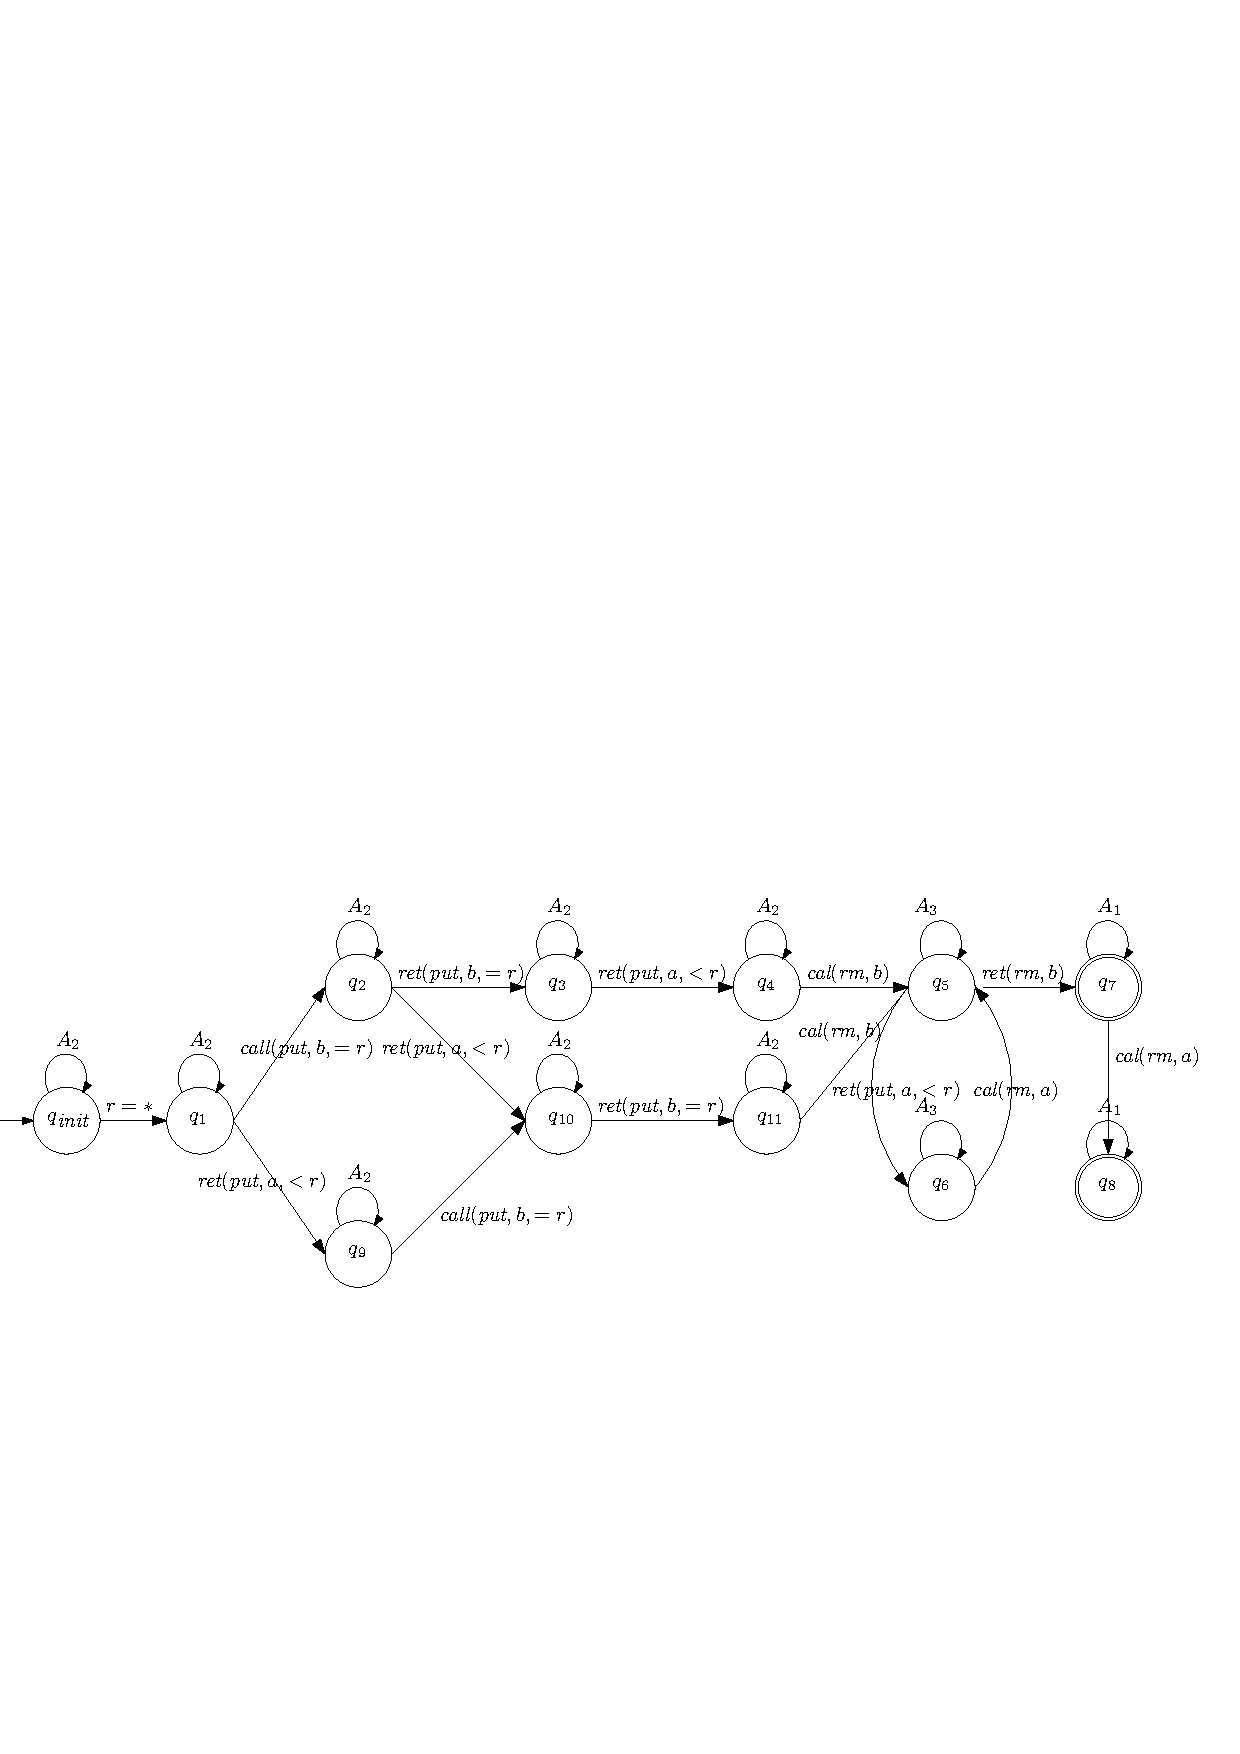
\includegraphics[width=1 \textwidth]{figures/PIC_AUTO_PQ1Lar-pprr.pdf}
%\vspace{-10pt}
  \caption{Automaton $\mathcal{A}_{\textit{l-lar}}^1$}
  \label{fig:automata APQ1Lar-1}
\end{figure}

$\mathcal{A}_{\textit{l-lar}}^1$ is used to recognize conditions in \figurename~\ref{fig:his for APQ1Lar-1}. Here for simplicity, we only draw operation of $b$, and the first $\textit{ret}(\textit{put},a)$.


\begin{figure}[htbp]
  \centering
  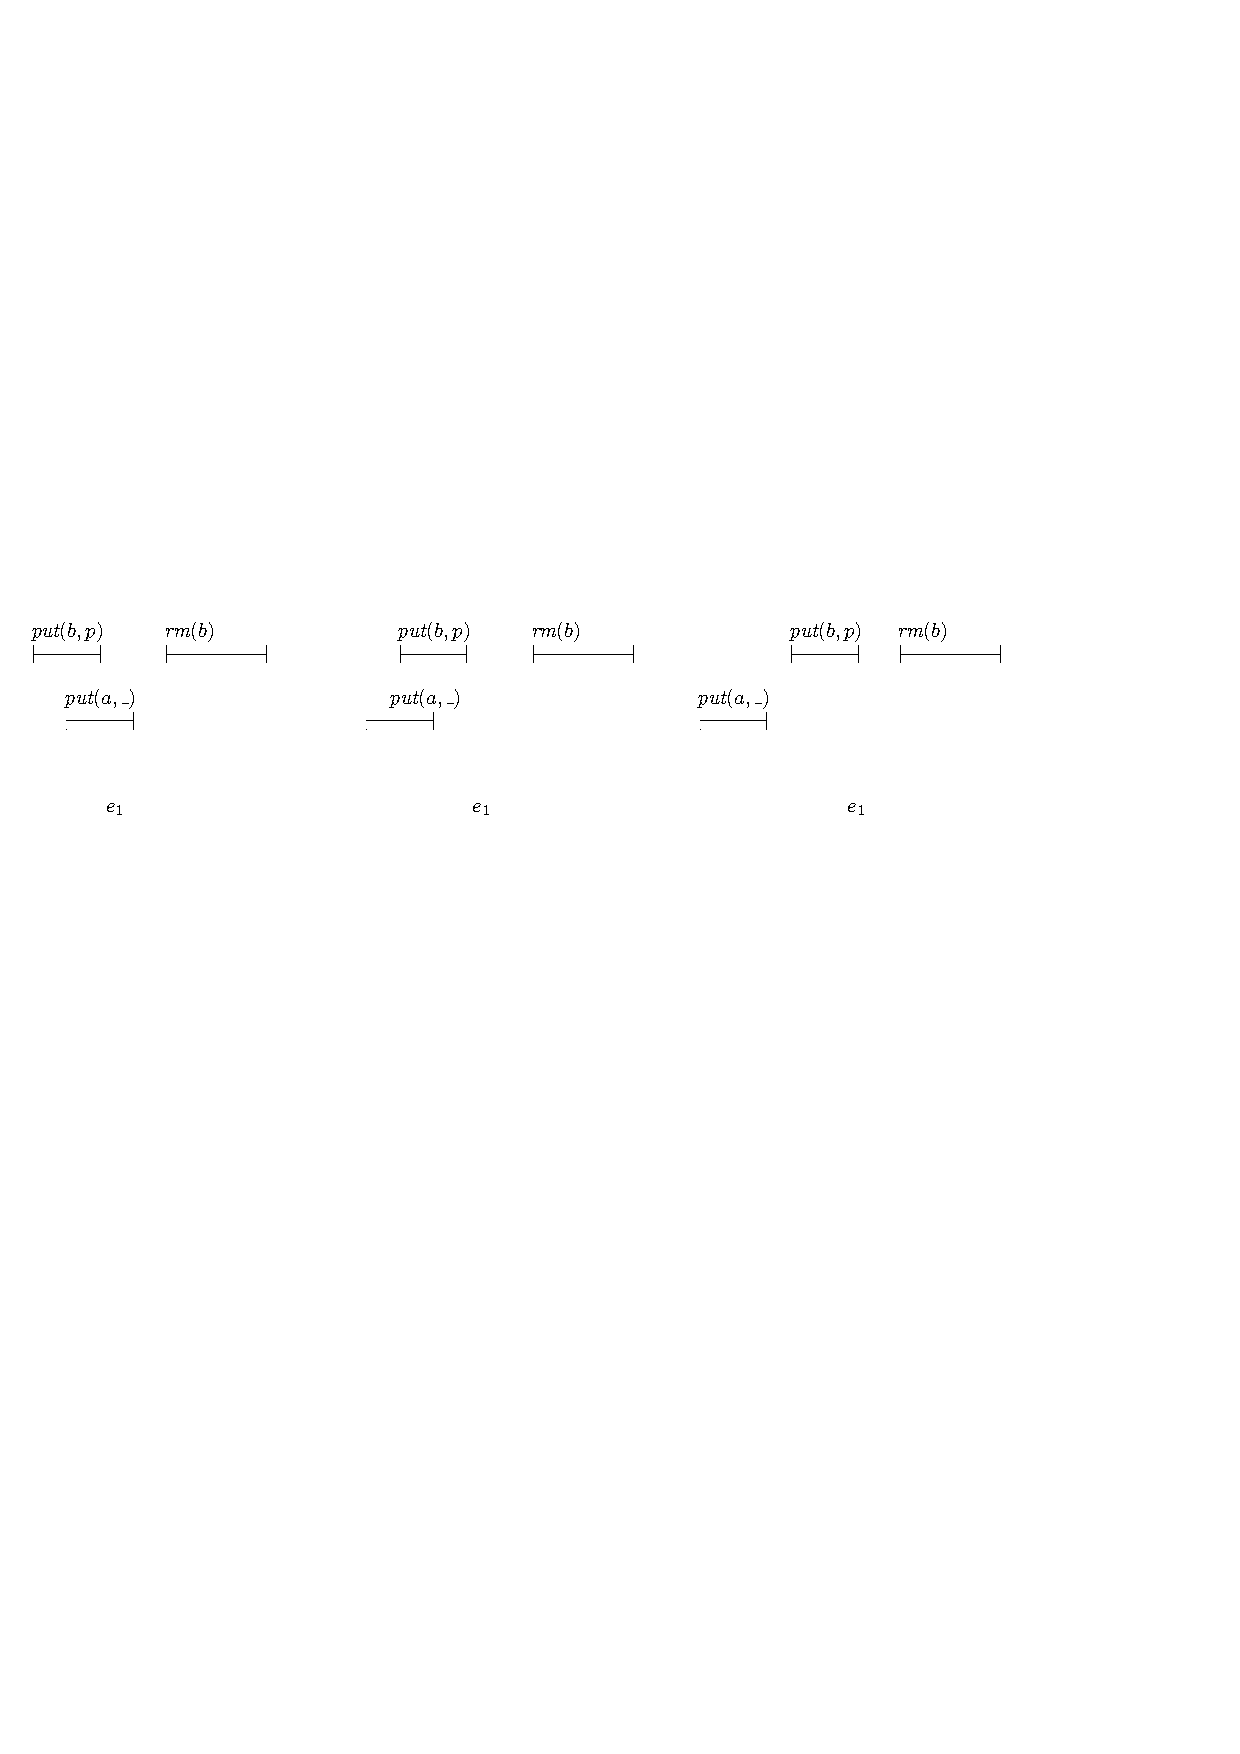
\includegraphics[width=1 \textwidth]{figures/PIC_HIS_PQ1Lar-pprr.pdf}
%\vspace{-10pt}
  \caption{Conditions recognized by $\mathcal{A}_{\textit{l-lar}}^1$}
  \label{fig:his for APQ1Lar-1}
\end{figure}


For the case when $e_r \vert_{b} = \textit{cal}(\textit{put},b,p) \cdot \textit{cal}(\textit{rm}) \cdot \textit{ret}(\textit{put}) \cdot \textit{ret}(\textit{rm},b)$, we generate witness automaton $\mathcal{A}_{\textit{l-lar}}^2$, as shown in \figurename~\ref{fig:automata APQ1Lar-2}. Here $c_1,c_2,c_3$ is the same as that in $\mathcal{A}_{\textit{l-lar}}^1$. The differentiated branch in $\mathcal{A}_{\textit{l-lar}}^2$ comes from the positions of the first $\textit{ret}(\textit{put},a)$.

\begin{figure}[htbp]
  \centering
  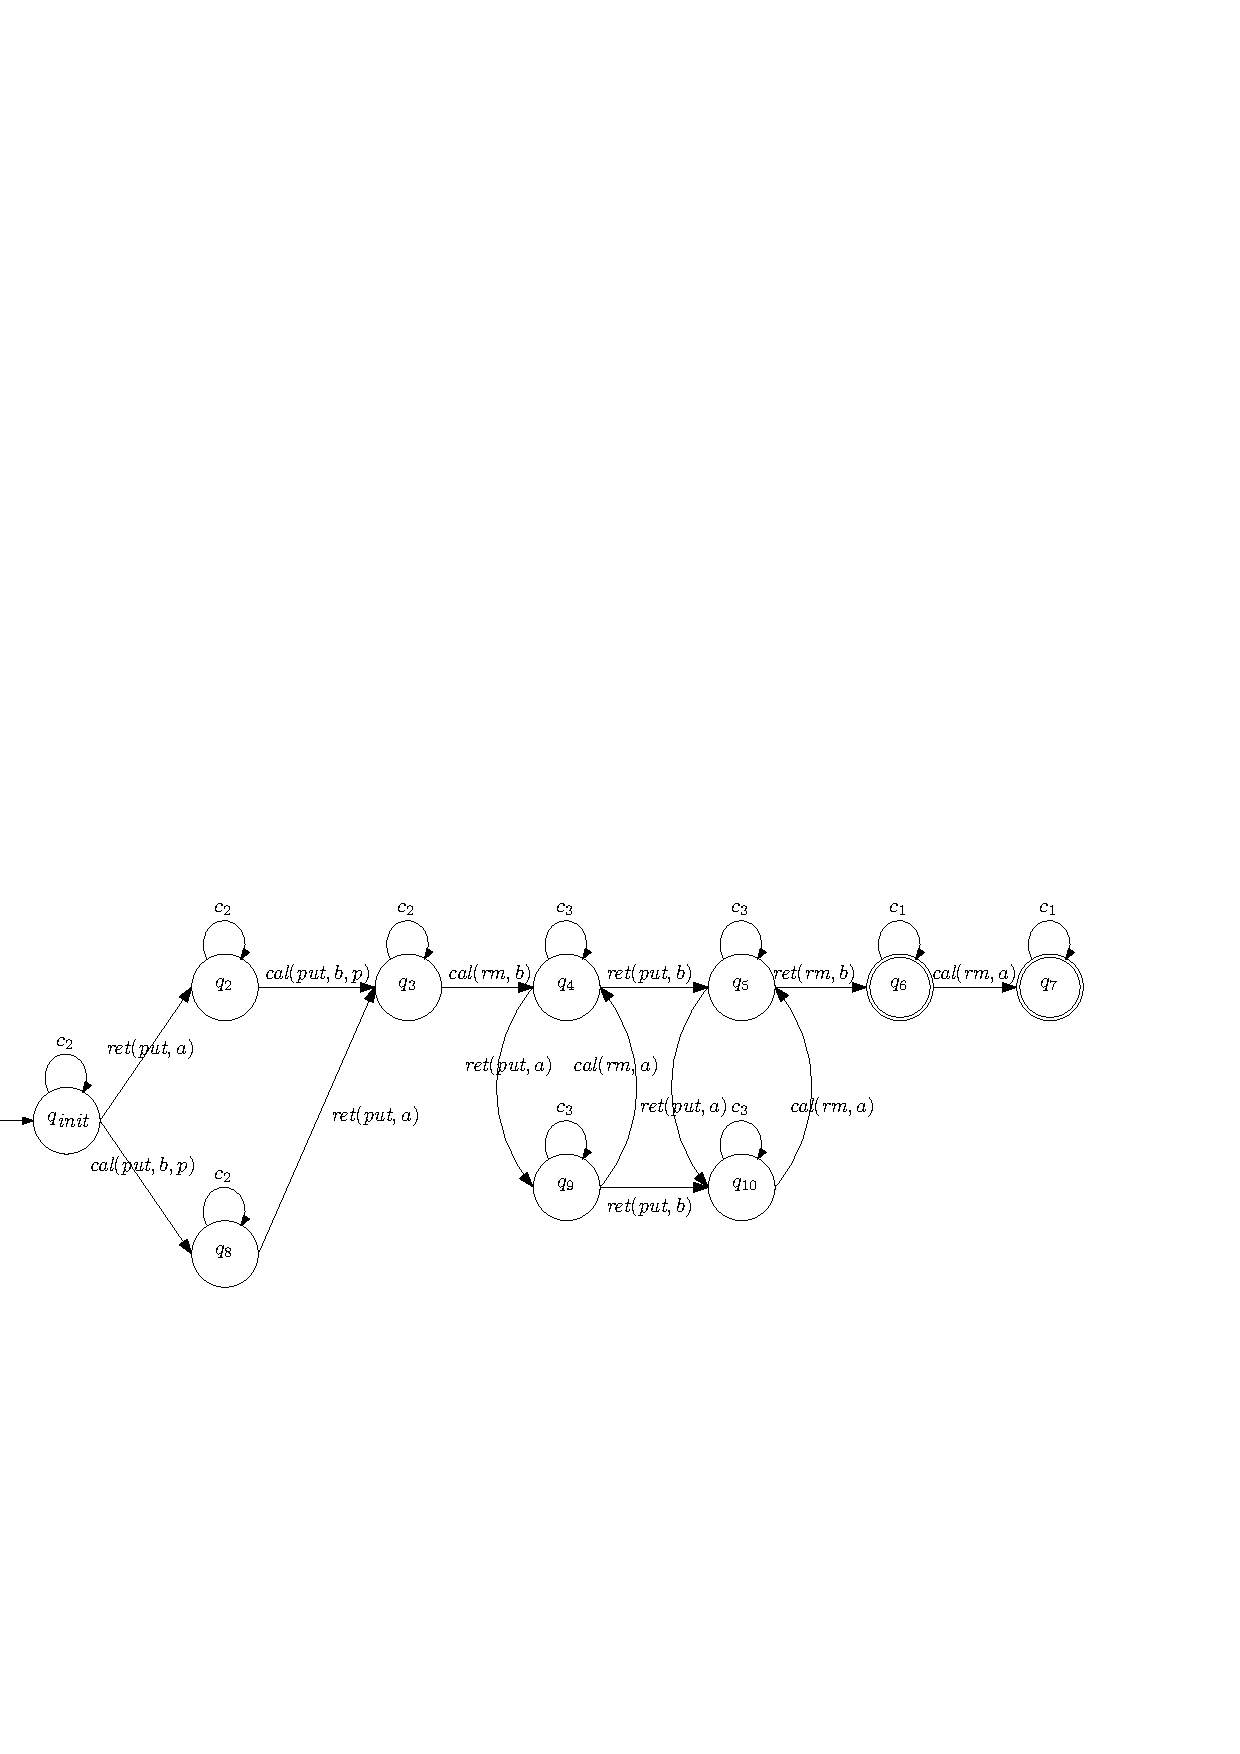
\includegraphics[width=1 \textwidth]{figures/PIC_AUTO_PQ1Lar-prpr.pdf}
%\vspace{-10pt}
  \caption{Automaton $\mathcal{A}_{\textit{l-lar}}^2$}
  \label{fig:automata APQ1Lar-2}
\end{figure}


$\mathcal{A}_{\textit{l-lar}}^2$ is used to recognize conditions in \figurename~\ref{fig:his for APQ1Lar-2}. Here for simplicity, we only draw operation of $b$, and the first $\textit{ret}(\textit{put},a)$.


\begin{figure}[htbp]
  \centering
  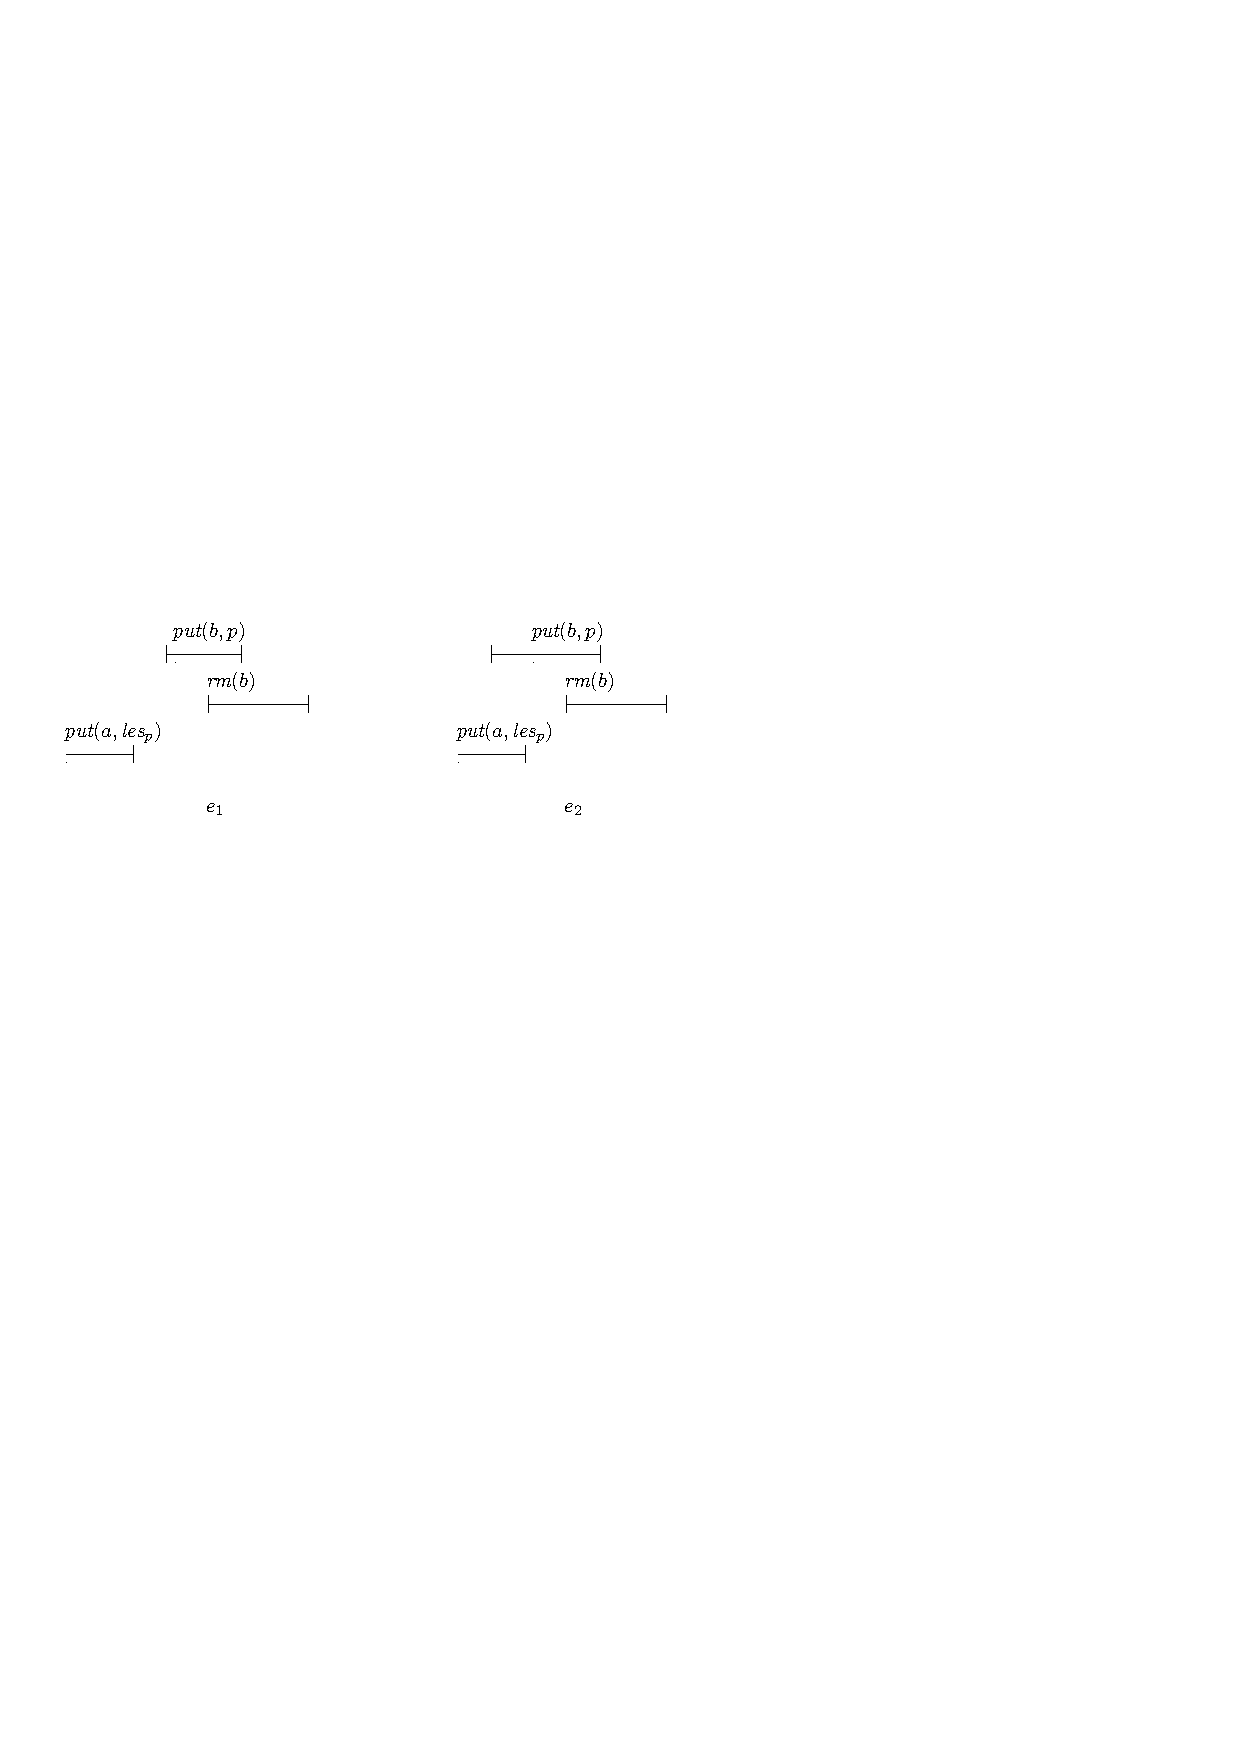
\includegraphics[width=0.7 \textwidth]{figures/PIC_HIS_PQ1Lar-prpr.pdf}
%\vspace{-10pt}
  \caption{Conditions recognized by $\mathcal{A}_{\textit{l-lar}}^2$}
  \label{fig:his for APQ1Lar-2}
\end{figure}

For the case when $e_r \vert_{b} = \textit{cal}(\textit{rm}) \cdot \textit{cal}(\textit{put},b,p) \cdot \textit{ret}(\textit{put}) \cdot \textit{ret}(\textit{rm},b)$, we generate witness automaton $\mathcal{A}_{\textit{l-lar}}^3$, as shown in \figurename~\ref{fig:automata APQ1Lar-3}. Here $c_1,c_2,c_3$ is the same as that in $\mathcal{A}_{\textit{l-lar}}^1$. The differentiated branch in $\mathcal{A}_{\textit{l-lar}}^3$ comes from the positions of the first $\textit{ret}(\textit{put},a)$.

\begin{figure}[htbp]
  \centering
  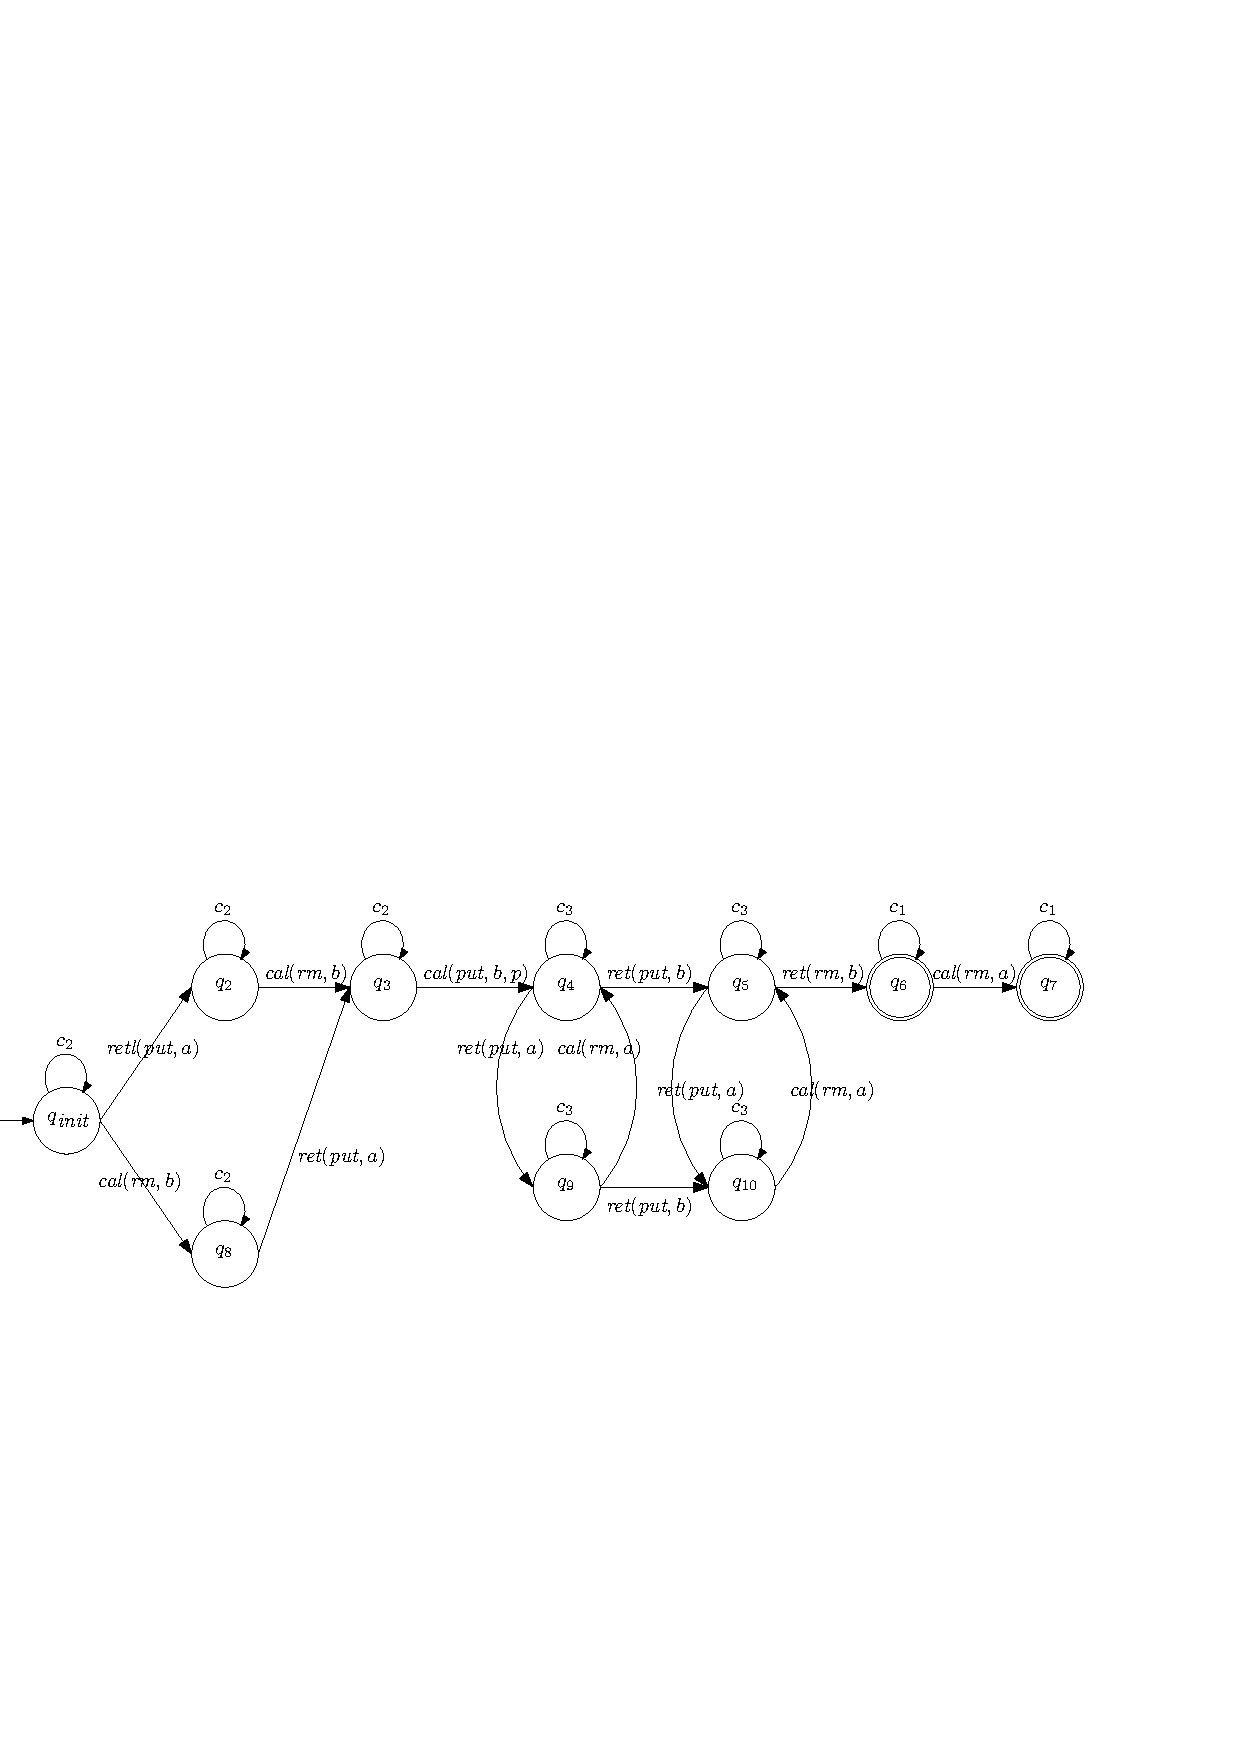
\includegraphics[width=1 \textwidth]{figures/PIC_AUTO_PQ1Lar-rppr.pdf}
%\vspace{-10pt}
  \caption{Automaton $\mathcal{A}_{\textit{l-lar}}^3$}
  \label{fig:automata APQ1Lar-3}
\end{figure}


$\mathcal{A}_{\textit{l-lar}}^3$ is used to recognize conditions in \figurename~\ref{fig:his for APQ1Lar-3}. Here for simplicity, we only draw operation of $b$, and the first $\textit{ret}(\textit{put},a)$.


\begin{figure}[htbp]
  \centering
  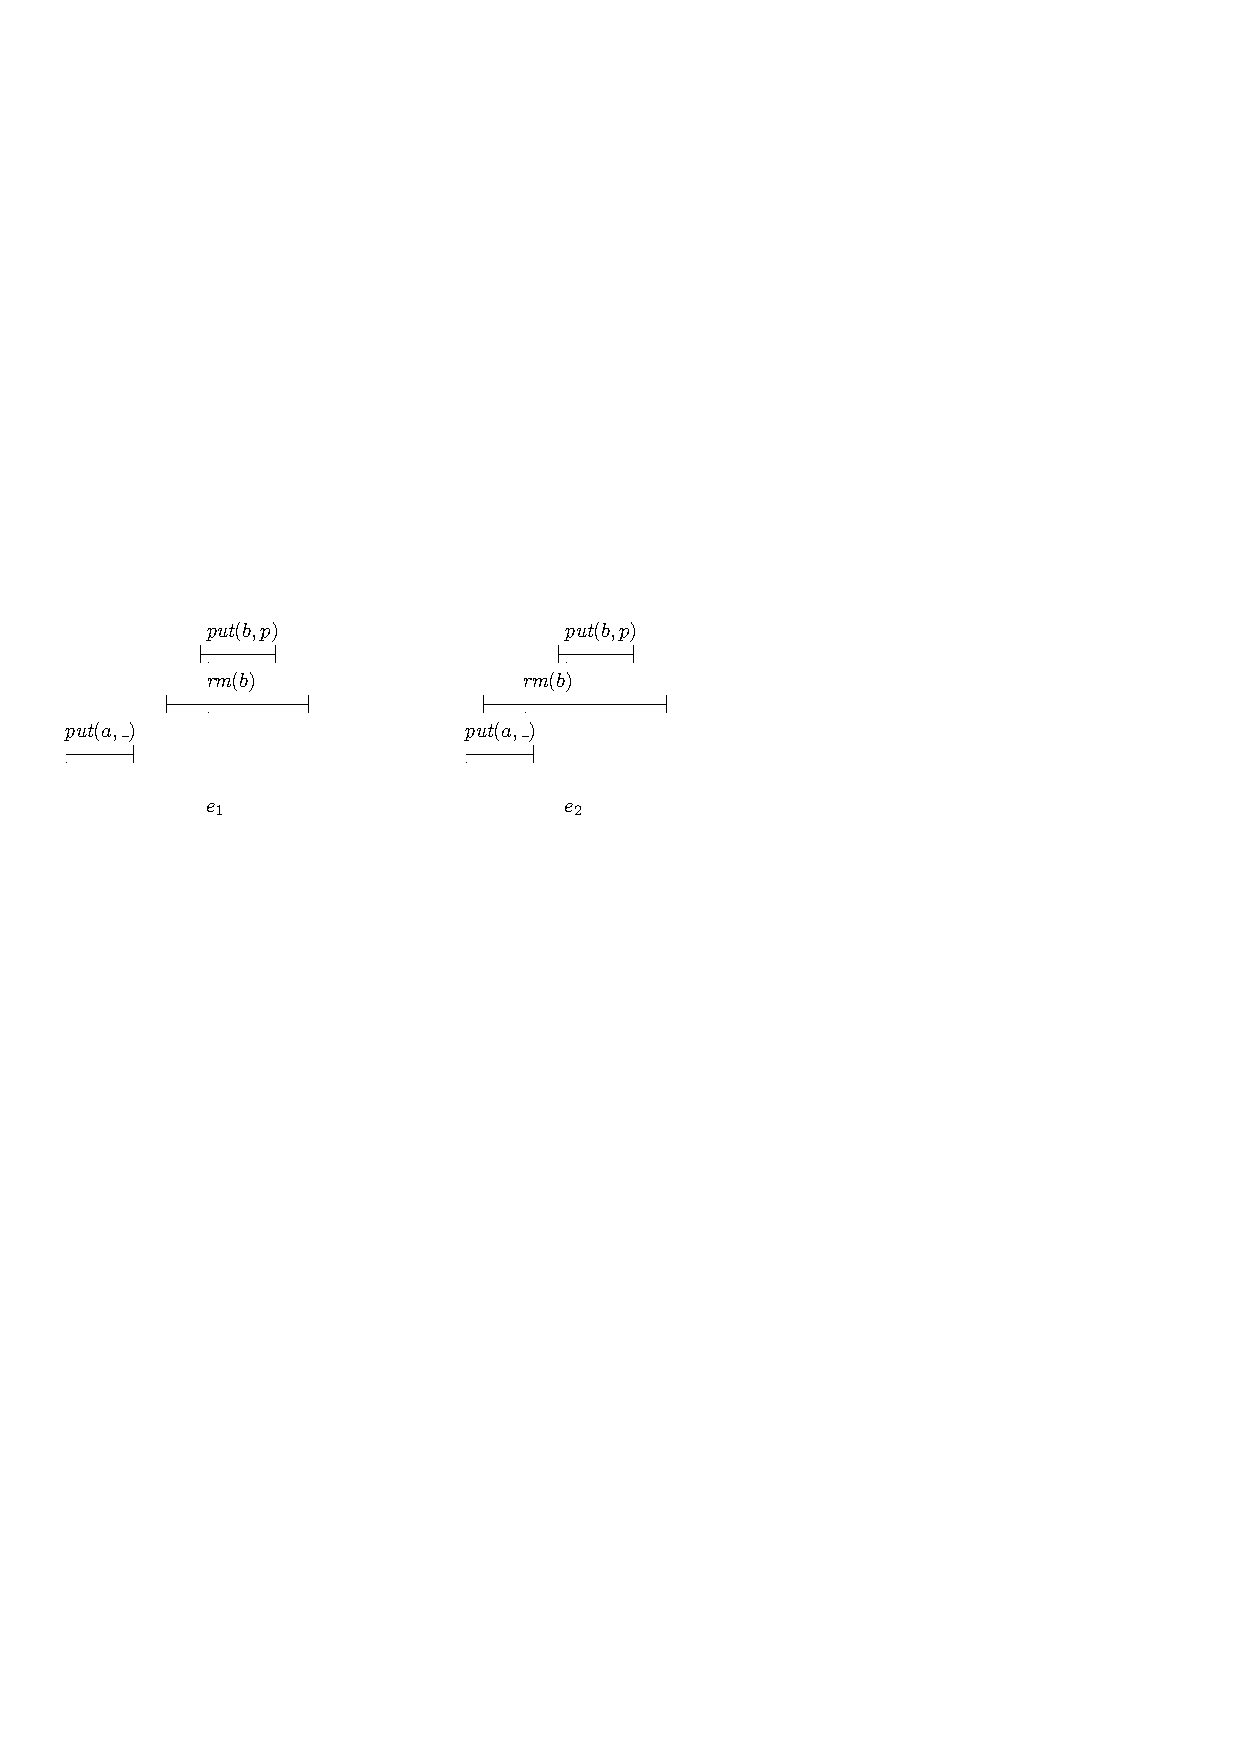
\includegraphics[width=0.7 \textwidth]{figures/PIC_HIS_PQ1Lar-rppr.pdf}
%\vspace{-10pt}
  \caption{Conditions recognized by $\mathcal{A}_{\textit{l-lar}}^3$}
  \label{fig:his for APQ1Lar-3}
\end{figure}


For the case when $e_r \vert_{b} = \textit{cal}(\textit{rm}) \cdot \textit{cal}(\textit{put},b,p) \cdot \textit{ret}(\textit{rm},b) \cdot \textit{ret}(\textit{put})$, we generate witness automaton $\mathcal{A}_{\textit{l-lar}}^4$, as shown in \figurename~\ref{fig:automata APQ1Lar-4}. Here $c_1,c_2,c_3$ is the same as that in $\mathcal{A}_{\textit{l-lar}}^1$, and $c_4 = c_1 + \textit{ret}(\textit{put},b)$. The differentiated branch in $\mathcal{A}_{\textit{l-lar}}^4$ comes from the positions of the first $\textit{ret}(\textit{put},a)$.

\begin{figure}[htbp]
  \centering
  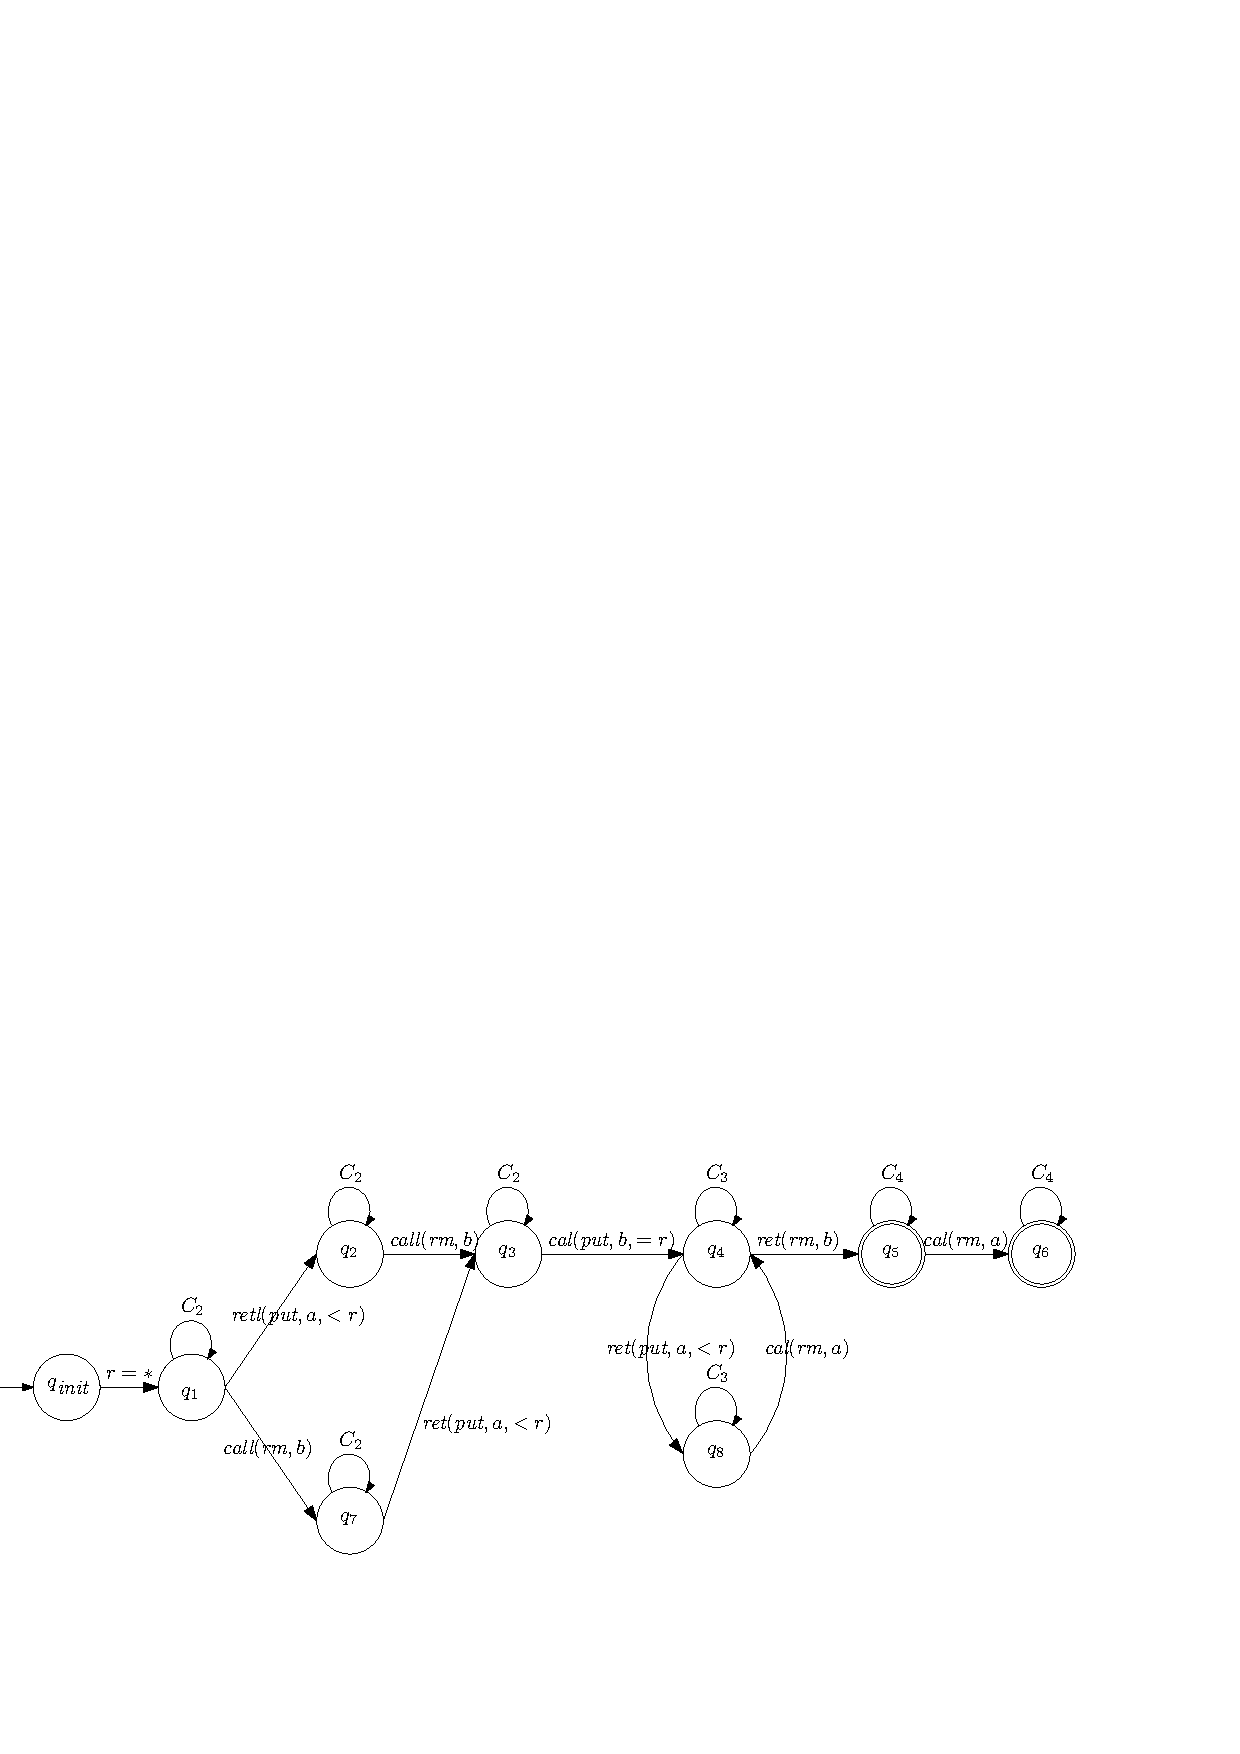
\includegraphics[width=0.9 \textwidth]{figures/PIC_AUTO_PQ1Lar-rprp.pdf}
%\vspace{-10pt}
  \caption{Automaton $\mathcal{A}_{\textit{l-lar}}^4$}
  \label{fig:automata APQ1Lar-4}
\end{figure}


$\mathcal{A}_{\textit{l-lar}}^4$ is used to recognize conditions in \figurename~\ref{fig:his for APQ1Lar-4}. Here for simplicity, we only draw operation of $b$, and the first $\textit{ret}(\textit{put},a)$.


\begin{figure}[htbp]
  \centering
  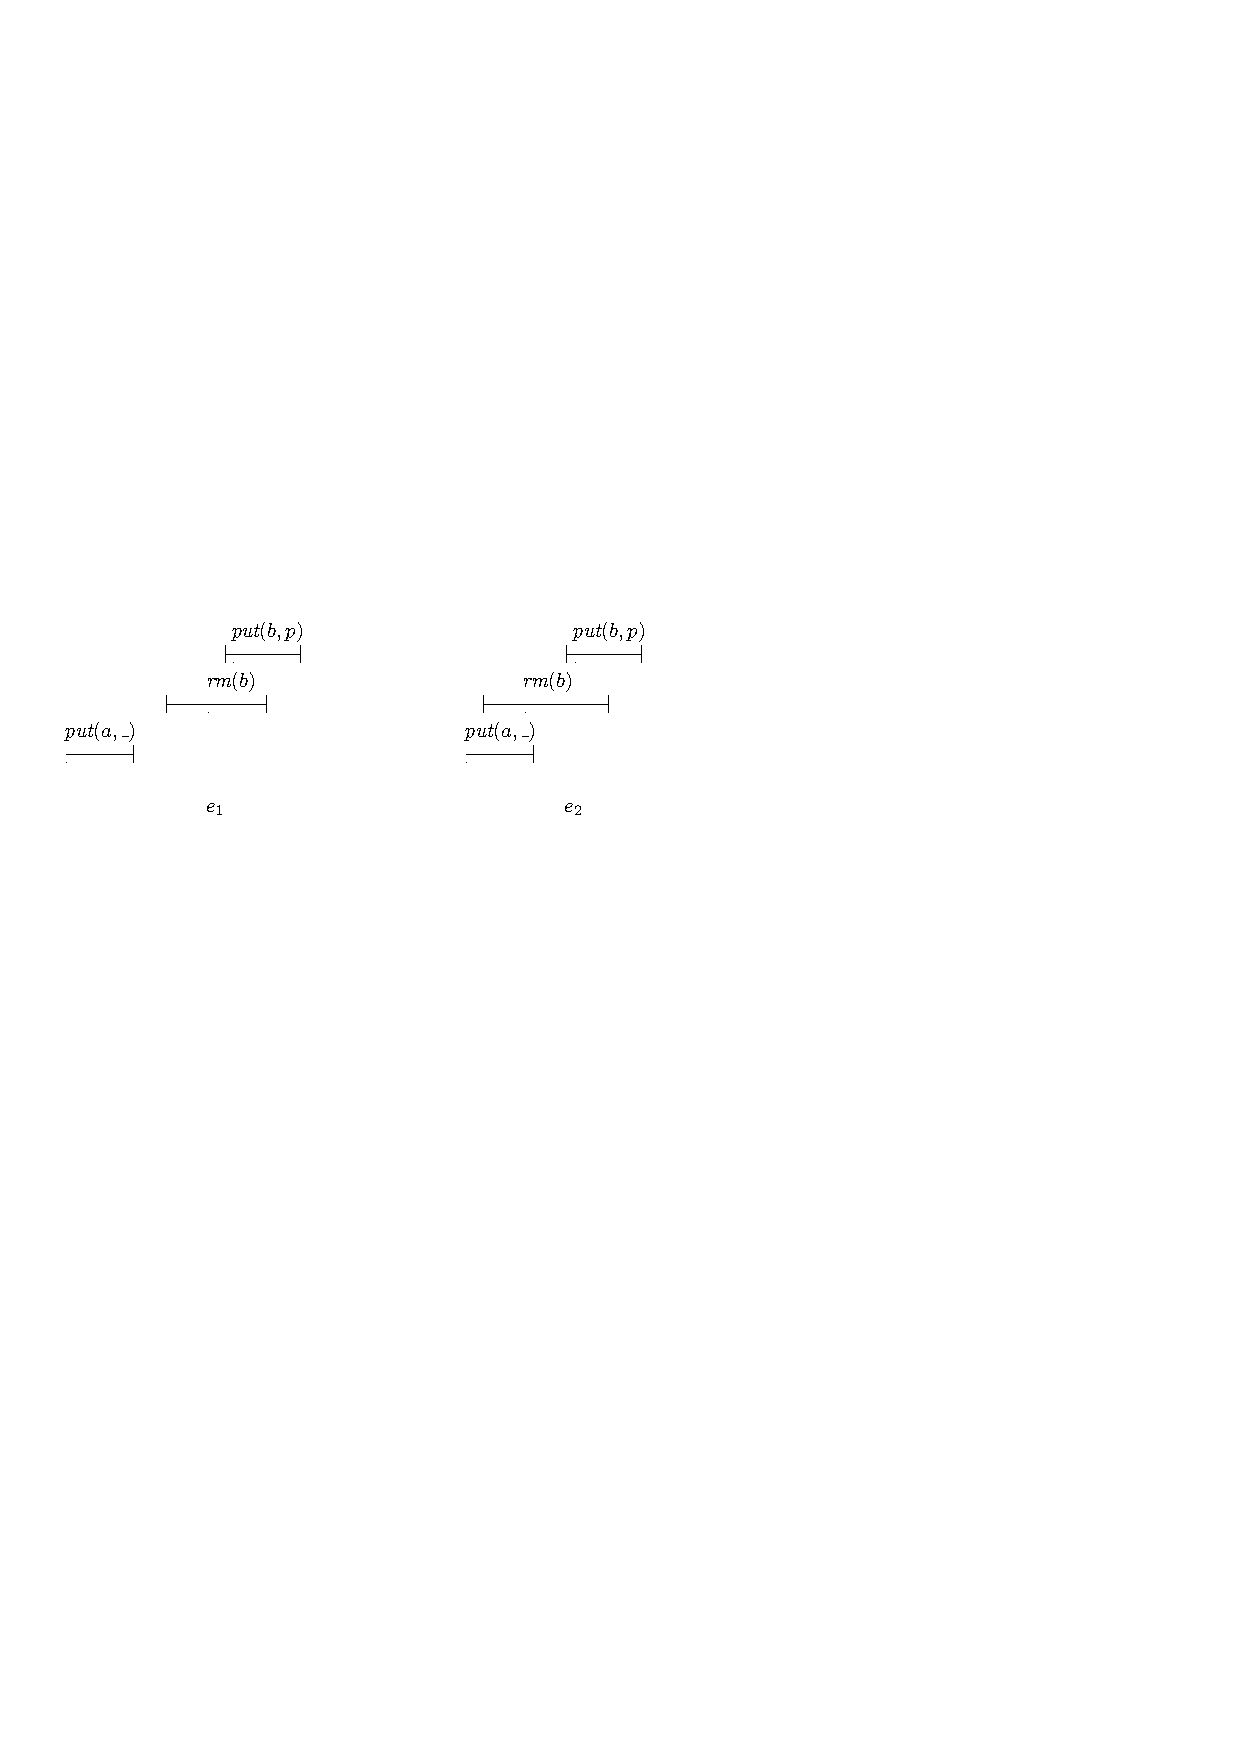
\includegraphics[width=0.7 \textwidth]{figures/PIC_HIS_PQ1Lar-rprp.pdf}
%\vspace{-10pt}
  \caption{Conditions recognized by $\mathcal{A}_{\textit{l-lar}}^4$}
  \label{fig:his for APQ1Lar-4}
\end{figure}

Let $\textit{Auts}_{\textit{1-lar}} = \{ \mathcal{A}_{\textit{l-lar}}^1, \mathcal{A}_{\textit{l-lar}}^2, \mathcal{A}_{\textit{l-lar}}^3, \mathcal{A}_{\textit{l-lar}}^4 \}$. The following lemma states that $\textit{EPQ}_1^{>}$ is co-regular.


\EPQOneLarisCoRegular*

\begin {proof}

We need to prove that, given a data-independence implementation $\mathcal{I}$, $\textit{Auts}_{\textit{1-lar}} \cap \mathcal{I} \neq \emptyset$, if and only if $\exists e \in \mathcal{I}_{\neq},$ $e' \in \textit{proj}(e),$ $\textit{EPQ}_1^{>} \in last(e') \wedge e'$ does not linearizable w.r.t. $\textit{MS}(\textit{EPQ}_1^{>})$.

By Lemma \ref{lemma:pri execution is enough} and Lemma \ref{lemma:Lin Equals Constraint for EPQ1Lar}, we need to prove the following fact:

\noindent {\bf $\textit{fact}_1$}: Given a data-independence implementation $\mathcal{I}$, $\textit{Auts}_{\textit{1-lar}} \cap \mathcal{I} \neq \emptyset$ if and only if $\exists e \in \mathcal{I}_{\neq},$ $e' \in \textit{proj}(e)$, $last(e')=\textit{EPQ}_1^{>}$, $x$ is the item with maximal priority $\textit{pri}$ in $e'$, $e'$ is a $\textit{pri}$-execution. And there is a cycle going through $x$ in $G$, where $G$ is the left-right constraint of $e'$.

\noindent The $\textit{only if}$ direction: Let us consider the case of $\mathcal{A}_{\textit{l-lar}}^1$. Assume that $e_1 \in \mathcal{I}$ is accepted by $\mathcal{A}_{\textit{l-lar}}^1$. By data-independence, there exists data-differentiated execution $e \in \mathcal{I}$ and renaming function $r_1$, such that $e_1 = r_1(e)$. Assume that $r_1$ maps $d$ into $b$ and maps $f_1,\ldots,f_m$ into $a$. Let $e'$ be obtained from $e$ by projection into $\{ d, f_1,\ldots,f_m \}$. Assume that the priority of $b$ is $p$. It is easy to see that $e'$ is a $p$-execution, $\textit{last}(e') = \textit{EPQ}_1^{>}$, and there is a cycle going through $d$ in $G$, where $G$ is the left-right constraint of $e'$. The case of $\mathcal{A}_{\textit{l-lar}}^2$, $\mathcal{A}_{\textit{l-lar}}^3$ and $\mathcal{A}_{\textit{l-lar}}^4$ can be similarly proved.

\noindent The $\textit{if}$ direction: Given such $e$, $e'$ and $x$. Let renaming function $r$ maps $x$ into $b$, maps items cover $x$ into $a$, and maps other items into $d$. By data-independence, $r(e) \in \mathcal{I}$. Then depending on the cases of $r(e) \vert_{b}$, we can see that $r(e)$ is accepted by $\mathcal{A}_{\textit{l-lar}}^1$, $\mathcal{A}_{\textit{l-lar}}^2$, $\mathcal{A}_{\textit{l-lar}}^3$ or $\mathcal{A}_{\textit{l-lar}}^4$. \qed
\end {proof}



\subsection{Proofs and Definitions in Subsection \ref{subsec:co-regular of EPQ1Equal}}
\label{sec:appendix proof and definition in section co-regular of EPQ1Equal}

Let $\textit{Items}(e,p)$ be the set of items with priority $p$ in execution $e$. The following lemma states a method to choose $\textit{itm}$ of $\textit{EPQ}_1^{=}$.

\begin{restatable}{lemma}{MaximalInPBadGPMakePQ1Equal}
\label{lemma:maximal in pb and gap-point make a candidate of EPQ1Equal}
Given a data-differentiated $\textit{pri}$-execution $e$ with $\textit{last}(e) = \textit{EPQ}_1^{=}$. If there exists an item $x$ with priority $\textit{pri}$, such that for each $y \in \textit{Items}(e,\textit{pri})$, (1) $x$ does not $<_{\textit{pb}}$ to $y$, and (2) the right-most gap-point of $x$ is after $\textit{cal}(\textit{put},y,\_)$ and $\textit{cal}(\textit{rm},y)$. Then $e \sqsubseteq \textit{MS}(\textit{EPQ}_1^{=})$.
\end{restatable}

\begin {proof}

Let $o$ be the right-most gap-point of $x$. We locate linearization points of each method event as follows:

\begin{itemize}
\setlength{\itemsep}{0.5pt}
\item[-] Locate the linearization point of $\textit{rm}(x)$ at $o$,

\item[-] If $\textit{put}(x,\textit{pri})$ overlaps with $\textit{rm}(x)$, then locate the linearization point of $\textit{put}(x,\textit{pri})$ just before the linearization point of $\textit{rm}(x)$. Otherwise, $\textit{put}(x,\textit{pri}) <_{\textit{hb}} \textit{rm}(x)$, and we locate the linearization point of $\textit{put}(x,\textit{pri})$ just before its return action.

\item[-] Locate linearization points of method event of each $y \in \textit{Items}(e,\textit{pri})$ (except for $x$) just after the call action of the method event.

\item[-] For item $z$ with priority smaller than $\textit{pri}$. If both $\textit{cal}(\textit{put},z,\_)$ and $\textit{cal}(\textit{rm},z)$ is before $o$, then locate the linearization points of $\textit{put}(z,\_)$ and $\textit{rm}(z)$ just after their call actions. If both $\textit{ret}(\textit{put},z)$ and $\textit{ret}(\textit{rm},z)$ (if exists) is after $o$, then locate the linearization points of $\textit{put}(z,\_)$ and $\textit{rm}(z)$ just before their return actions. Otherwise, $x$ is in interval of $z$, which contradicts the definition of gap-point, and is impossible.
\end{itemize}

Let $l$ be the sequence of linearization points constructed above. It is obvious that $e \sqsubseteq l$. Since for each $y \in \textit{Items}(e,\textit{pri})$, $o$ is after $\textit{cal}(\textit{put},y,\_)$ and $\textit{cal}(\textit{rm},x)$, we can see that $\textit{rm}(x)$ is after $\textit{put}(y,\textit{pri})$ and $\textit{rm}(y)$ in $l$. It is obvious that $\textit{put}(x,\textit{pri})$ is before $\textit{rm}(x)$ in $l$. Since $x$ does not $<_{\textit{pb}}$ to $y$, we can see that no $\textit{put}(y,\textit{pri})$ happens before $\textit{put}(x,\textit{pri})$. Then it is easy to see that $\textit{put}(x,\textit{pri})$ is after $\textit{put}(y,\textit{pri})$ in $l$. Since $\textit{last}(e) = \textit{EPQ}_1^{=}$, all other items in $\textit{Items}(e,\textit{pri})$ has matched $\textit{put}$ and $\textit{rm}$, and it is easy to see that their $\textit{put}$ and $\textit{rm}$ (except for that of $x$) are all before $\textit{rm}(x)$ in $l$.

For item $z$ with priority smaller than $\textit{pri}$, we can see that there are only two possibilities: (1) $\textit{put}(z,\_)$ and $\textit{rm}(z)$ are both before $\textit{rm}(x)$ in $l$, and (2) $\textit{put}(z,\_)$ and $\textit{rm}(z)$ (if exists) are after before $\textit{rm}(x)$ in $l$. Therefore, before $\textit{rm}(x)$ in $l$, the $\textit{put}$ and $\textit{rm}$ of $z$ are matched.

Therefore, it is easy to see that $l \in \textit{MS}(\textit{EPQ}_1^{=})$. \qed
\end {proof}

With Lemma \ref{lemma:maximal in pb and gap-point make a candidate of EPQ1Equal}, we can prove the following lemma, which states that getting rid of case in \figurename~\ref{fig:introduce pb order} is enough for ensure $\textit{last}(e) = \textit{EPQ}_1^{=} \Rightarrow e \sqsubseteq \textit{MS}(\textit{EPQ}_1^{=})$.


\EPQOneEqualAsPBandGP*

\begin {proof}

To prove the $\textit{if}$ direction, let $e_{x,y}$ be the execution that is obtained from $e$ by erasing all actions of items that has same priority as $x$, except for actions of $x$ and $y$. It is obvious that $\textit{last}(e_{x,y}) = \textit{EPQ}_1^{=}$. Since $y <_{\textit{pb}}^* x$, according to $\textit{EPQ}_1^{=}$, we can see that $x$ should be chosen as $\textit{itm}$ in $\textit{EPQ}_1^{=}$.

According to Lemma \ref{lemma:Lin Equals Constraint for EPQ1Lar} (Here we temporarily forget the existence of $y$), the only possible position for locating linearizaton point of $\textit{rm}(x)$ is at gap-point of $x$. Otherwise, if the linearizaton point of $\textit{rm}(x)$ is chosen at a position that is not a gap-point of $x$, then there exists unmatched method event before $\textit{rm}(x)$ with smaller priority. Since the rightmost gap-point of $x$ is before $\textit{cal}(\textit{put},y,\textit{pri})$ or $\textit{cal}(\textit{rm},y)$, if we locate linearizaton point of $\textit{rm}(x)$ at gap-point of $x$, then $\textit{rm}(x)$ will be before $\textit{cal}(\textit{put},y,\textit{pri})$ or $\textit{cal}(\textit{rm},x)$.

Therefore, for every sequence $l = u \cdot \textit{put}(x,\textit{pri}) \cdot v \cdot \textit{rm}(x) \cdot w$, if $e_{x,y} \sqsubseteq l$, then either $u \cdot v$ contains some unmatched method events of priority smaller than $\textit{pri}$, or $w$ contains $\textit{put}(y,\textit{pri})$ or $\textit{rm}(y)$. In both cases, $l \notin \textit{MS}(\textit{EPQ}_1^{=})$.

To prove the $\textit{only if}$ direction, we prove its contrapositive. Assume we already know that for each $x$ and $y$ has maximal priority in $e$, if $y <_{\textit{pb}}^* x$, then the rightmost gap-point of $x$ is after $\textit{cal}(\textit{put},y,\textit{pri})$ and $\textit{cal}(\textit{rm},x)$. We need to prove that $e \sqsubseteq \textit{MS}(\textit{EPQ}_1^{=})$. Recall that we already assume that each single-priority execution has FIFO property, and item with larger priority is not covered by items with smaller priority.

Our proof proceed as follows:

\begin{itemize}
\setlength{\itemsep}{0.5pt}
\item[-] Let $e_{\textit{pri}}$ be the projection of $e$ into operations of priority $\textit{pri}$. Since each single-priority execution has FIFO property, there exists sequence $l_{\textit{pri}}$, such that $e_{\textit{pri}} \sqsubseteq l_{\textit{pri}}$, and when we treat $\textit{put}$ as $\textit{enq}$ and $\textit{rm}$ as $\textit{deq}$, $l_{\textit{pri}}$ belongs to queue.

\item[-] Let $a_1$ be the last inserted item of $l_{\textit{pri}}$.

    Step $1$: Check whether for each $b \in \textit{Items}(e,\textit{pri})$, (1) $a_1$ does not $<_{\textit{pb}}$ to $b$, and (2) the right-most gap-point of $a$ is after $\textit{cal}(\textit{put},b,\textit{pri})$ and $\textit{cal}(\textit{rm},b)$.

    It is easy to see that $a_1$ is of priority $\textit{pri}$, and $a_1$ does not $<_{\textit{pb}}$ to any $b \in \textit{Items}(e,\textit{pri})$. If for each $b \in \textit{Items}(e,\textit{pri})$, the rightmost gap-point of $a_1$ is after $\textit{cal}(\textit{put},b,\textit{pri})$ and $\textit{cal}(\textit{rm},b)$. Then by Lemma \ref{lemma:maximal in pb and gap-point make a candidate of EPQ1Equal}, we can obtain that $e \sqsubseteq \textit{MS}(\textit{EPQ}_1^{=})$.


\item[-] Otherwise, there exists $a_2 \in \textit{Items}(e,\textit{pri})$, such that the rightmost gap-point of $a_1$ is before $\textit{cal}(\textit{put},a_2,\textit{pri})$ or $\textit{cal}(\textit{rm},a_2)$ in $e$. We can see that each gap-point of $a_2$ is after the rightmost gap-point of $a_1$.%, and thus, the right-most gap-point of $a_2$ is after the rightmost gap-point of $a_1$.
    By assumption, we know that $a_2$ does not $<_{\textit{pb}}$ to $a_1$.

    \begin{itemize}
    \setlength{\itemsep}{0.5pt}
    \item[-] If for each item $b \in \textit{Items}(e,\textit{pri})$, $a_2$ does not $<_{\textit{pb}}$ to $b$. Then we go to step $1$ and treat $a_2$ similarly as $a_1$.
    \item[-] Otherwise, there exists $a_3$ with priority $\textit{pri}$ such that $a_2 <_{\textit{pb}}^* a_3$.

    Since $l_{\textit{pri}}$ has FIFO property, it is easy to see that there is no cycle in $<_{\textit{pb}}$ order. It is safe to assume that $a_3$ is maximal in the sense of $<_{\textit{pb}}^*$. Or we can say, there does not exists $a_4$, such that $a_3 <_{\textit{pb}}^* a_4$.

    By assumption,we know that the rightmost gap-point of $a_3$ is after $\textit{cal}(\textit{put},a_2,\textit{pri})$ and $\textit{cal}(\textit{rm},a_2)$. Therefore, we can see that the rightmost gap-point of $a_3$ is after the rightmost gap-point of $a_1$. Then we go to step $1$ and treat $a_3$ similarly as $a_1$.
    \end{itemize}
\end{itemize}

Let $a^i$ be the $a_1$ in the $\textit{i-th}$ loop of our proof. It is not hard to see that, given $i<j$, the rightmost gap-point of $a^j$ is after the rightmost gap-point of $a^i$. Therefore, the loop finally stop at some $a^f$. $a^f$ satisfies the check of Step $1$. By Lemma \ref{lemma:maximal in pb and gap-point make a candidate of EPQ1Equal}, this implies that $e \sqsubseteq \textit{MS}(\textit{EPQ}_1^{=})$. This completes the proof of $\textit{if}$ direction. \qed
\end {proof}



According to the definition of $<_{\textit{ob}}^*$, if $a <_{\textit{pb}}^* b$, then there exists $a_1,\ldots,a_m$, such that $a <_{\textit{pb}} a_1 <_{\textit{pb}} \ldots <_{\textit{pb}} a_m <_{\textit{pb}} b$. The following lemma states that, the number of intermediate items $a_i$ is in fact bounded.

\OBOrderHasBoundedLength*

\begin {proof}

Our proof proceed as follows:

\begin{itemize}
\setlength{\itemsep}{0.5pt}
\item[-] ($<_{\textit{pb}}^A \cdot <_{\textit{pb}}^A$,$<_{\textit{pb}}^B \cdot <_{\textit{pb}}^B$ and $<_{\textit{pb}}^C \cdot <_{\textit{pb}}^C$): If $c_3 <_{\textit{pb}}^A c_2 <_{\textit{pb}}^A c_1$, then $\textit{put}(c_3,\_)$ happens before $\textit{put}(c_2,\_)$, and $\textit{put}(c_2,\_)$ happens before $\textit{put}(c_1,\_)$. Therefore, it is obvious that $\textit{put}(c_3,\_)$ happens before $\textit{put}(c_1,\_)$ and $c_3 <_{\textit{pb}}^A c_1$.

    Similarly, if $c_3 <_{\textit{pb}}^B c_2 <_{\textit{pb}}^B c_1$, then $c_3 <_{\textit{pb}}^B c_1$.

    If $c_3 <_{\textit{pb}}^C c_2 <_{\textit{pb}}^C c_1$: Since $c_2 <_{\textit{pb}}^C c_1$, $\textit{ret}(\textit{rm},c_2)$ is before $\textit{cal}(\textit{put},c_1,\_)$. Since $\textit{rm}(c_2)$ does not happen before $\textit{put}(c_2,\_)$, $\textit{cal}(\textit{put},c_2,\_)$ is before $\textit{ret}(\textit{rm},c_2)$. Since $c_3 <_{\textit{pb}}^C c_2$, $\textit{ret}(\textit{rm},c_3)$ is before $\textit{cal}(\textit{put},c_2,\_)$. Therefore, $\textit{ret}(\textit{rm},c_3)$ is before $\textit{cal}(\textit{put},c_1,\_)$, and $c_3 <_{\textit{pb}}^C c_1$.

    Therefore, when we meet successive $<_{\textit{pb}}^A$, it is safe to leave only the first and the last elements and ignore intermediate elements. Similar cases hold for $<_{\textit{pb}}^B$ and $<_{\textit{pb}}^C$.

\item[-] $<_{\textit{pb}}^A$ and $<_{\textit{pb}}^C$:

    \begin{itemize}
    \setlength{\itemsep}{0.5pt}
    \item[-] ($<_{\textit{pb}}^A \cdot <_{\textit{pb}}^C$): If $c_3 <_{\textit{pb}}^A c_2 <_{\textit{pb}}^C c_1$. Since $c_2 <_{\textit{pb}}^C c_1$, $\textit{ret}(\textit{rm},c_2)$ is before $\textit{cal}(\textit{put},c_1,\_)$. Since $\textit{rm}(c_2)$ does not happen before $\textit{put}(c_2,\_)$, $\textit{cal}(\textit{put},c_2,\_)$ is before $\textit{ret}(\textit{rm},c_2)$. Since $c_3 <_{\textit{pb}}^A c_2$, $\textit{ret}(\textit{put},c_3)$ is before $\textit{cal}(\textit{put},c_2,\_)$. Therefore, $\textit{ret}(\textit{put},c_3)$ is before $\textit{cal}(\textit{put},c_1,\_)$, and $c_3 <_{\textit{pb}}^A c_1$.

    \item[-] ($<_{\textit{pb}}^C \cdot <_{\textit{pb}}^A$): If $c_3 <_{\textit{pb}}^C c_2 <_{\textit{pb}}^A c_1$. Since $c_2 <_{\textit{pb}}^A c_1$, $\textit{ret}(\textit{put},c_2)$ is before $\textit{cal}(\textit{put},c_1,\_)$. It is obvious that $\textit{cal}(\textit{put},c_2,\_)$ is before $\textit{ret}(\textit{put},c_2)$. Since $c_3 <_{\textit{pb}}^C c_2$, $\textit{ret}(\textit{rm},c_3)$ is before $\textit{cal}(\textit{put},c_2,\_)$. Therefore, $\textit{ret}(\textit{rm},c_3)$ is before $\textit{cal}(\textit{put},c_1,\_)$, and $c_3 <_{\textit{pb}}^C c_1$.

    %Since $c_2 <_{\textit{pb}}^A c_1$, $\textit{put}(c_2,\_)$ happens before $\textit{put}(c_1,\_)$. Since $c_3 <_{\textit{pb}}^C c_2$, $\textit{rm}(c_3)$ happens before $\textit{put}(c_2,\_)$. Therefore, $\textit{rm}(c_3)$ happens before $\textit{put}(c_1,\_)$, and $c_3 <_{\textit{pb}}^C c_1$.
    \end{itemize}

\item[-] $<_{\textit{pb}}^B$ and $<_{\textit{pb}}^C$:

    \begin{itemize}
    \setlength{\itemsep}{0.5pt}
    \item[-] ($<_{\textit{pb}}^B \cdot <_{\textit{pb}}^C$): If $c_3 <_{\textit{pb}}^B c_2 <_{\textit{pb}}^C c_1$. Since $c_2 <_{\textit{pb}}^C c_1$, $\textit{ret}(\textit{rm},c_2)$ is before $\textit{cal}(\textit{put},c_1,\_)$. It is obvious that $\textit{cal}(\textit{rm},c_2)$ is before $\textit{ret}(\textit{rm},c_2)$. Since $c_3 <_{\textit{pb}}^B c_2$, $\textit{ret}(\textit{rm},c_3)$ is before $\textit{cal}(\textit{rm},c_2)$. Therefore, $\textit{ret}(\textit{rm},c_3)$ is before $\textit{cal}(\textit{put},c_1,\_)$, and $c_3 <_{\textit{pb}}^C c_1$.

    \item[-] ($<_{\textit{pb}}^C \cdot <_{\textit{pb}}^B$): If $c_3 <_{\textit{pb}}^C c_2 <_{\textit{pb}}^B c_1$. Since $c_2 <_{\textit{pb}}^B c_1$, $\textit{ret}(\textit{rm},c_2)$ is before $\textit{cal}(\textit{rm},c_1)$. Since $\textit{rm}(c_2)$ does not happen before $\textit{put}(c_2,\_)$, $\textit{cal}(\textit{put},c_2,\_)$ is before $\textit{ret}(\textit{rm},c_2)$. Since $c_3 <_{\textit{pb}}^C c_2$, $\textit{ret}(\textit{rm},c_3)$ is before $\textit{cal}(\textit{put},c_2,\_)$. Therefore, $\textit{ret}(\textit{rm},c_3)$ is before $\textit{cal}(\textit{rm},c_1)$, and $c_3 <_{\textit{pb}}^B c_1$.
    \end{itemize}

\item[-]  ($<_{\textit{pb}}^A \cdot <_{\textit{pb}}^B \cdot <_{\textit{pb}}^A$): If $c_4 <_{\textit{pb}}^A c_3 <_{\textit{pb}}^B c_2 <_{\textit{pb}}^A c_1$:
    \begin{itemize}
    \setlength{\itemsep}{0.5pt}
    \item[-] If $\textit{cal}(\textit{rm},c_2)$ is before $\textit{cal}(\textit{put},c_1,\_)$: Since $c_3 <_{\textit{pb}}^B c_2$, $\textit{ret}(\textit{rm},c_3)$ is before $\textit{cal}(\textit{rm},c_2)$. Then $\textit{ret}(\textit{rm},c_3)$ is before $\textit{cal}(\textit{put},c_1,\_)$, and $c_3 <_{\textit{pb}}^C c_1$. This implies that $c_4 <_{\textit{pb}}^A c_3 <_{\textit{pb}}^C c_1$. According to the fact for $<_{\textit{pb}}^A \cdot <_{\textit{pb}}^C$, we know that $c_4  <_{\textit{pb}}^A c_1$.

    \item[-] If $\textit{cal}(\textit{rm},c_2)$ is after $\textit{cal}(\textit{put},c_1,\_)$: Since $c_2 <_{\textit{pb}}^A c_1$, $\textit{ret}(\textit{put},c_2,\_)$ is before $\textit{cal}(\textit{put},c_1,\_)$. Since $c_3 <_{\textit{pb}}^B c_2$, $\textit{rm}(c_3)$ happens before $\textit{rm}(c_2)$, and then we know that $\textit{put}(c_2,\_)$ can not happen before $\textit{put}(c_3,\_)$. Since $\textit{put}(c_2,\_)$ does not happen before $\textit{put}(c_3,\_)$, $\textit{cal}(\textit{put},c_3,\_)$ is before $\textit{ret}(\textit{put},c_2,\_)$. Since $c_4 <_{\textit{pb}}^A c_3$, $\textit{ret}(\textit{put},c_4)$ is before $\textit{cal}(\textit{put},c_3,\_)$. Therefore, $\textit{ret}(\textit{put},c_4)$ is before $\textit{cal}(\textit{put},c_1,\_)$, and $c_4 <_{\textit{pb}}^A c_1$.
    \end{itemize}

\item[-]  ($<_{\textit{pb}}^B \cdot <_{\textit{pb}}^A \cdot <_{\textit{pb}}^B$): If $c_4 <_{\textit{pb}}^B c_3 <_{\textit{pb}}^A c_2 <_{\textit{pb}}^B c_1$: Since $c_2 <_{\textit{pb}}^B c_1$, $\textit{ret}(\textit{rm},c_2)$ is before $\textit{cal}(\textit{rm},c_1)$. Since $c_3 <_{\textit{pb}}^A c_2$, we can see that $\textit{put}(c_3,\_) <_{\textit{hb}} \textit{put}(c_2,\_)$. Since each single-priority execution has FIFO property, we know that $\textit{rm}(c_2)$ does not happen before $\textit{rm}(c_3)$, and thus, $\textit{cal}(\textit{rm},c_3)$ is before $\textit{ret}(\textit{rm},c_2)$. Since $c_4 <_{\textit{pb}}^B c_3$, $\textit{ret}(\textit{rm},c_4)$ is before $\textit{cal}(\textit{rm},c_3)$. Therefore, $\textit{ret}(\textit{rm},c_4)$ is before $\textit{cal}(\textit{rm},c_1)$, and $c_4 <_{\textit{pb}}^B c_1$.

\end{itemize}

Based on above results, given $a <_{\textit{pb}}^{b_1} a_1 <_{\textit{pb}} \ldots <_{\textit{pb}}^{b_m} a_m <_{\textit{pb}}^{b_{\textit{m+1}}} b$, where each $b_i$ is in $\{ A,B,C \}$, we can merge relations, until we got one of the following facts:

\begin{itemize}
\setlength{\itemsep}{0.5pt}
\item[-] $a <_{\textit{pb}}^A b$, $a <_{\textit{pb}}^B b$ or $a <_{\textit{pb}}^C b$,

\item[-] $a <_{\textit{pb}}^A a_i <_{\textit{pb}}^B b$, or $a <_{\textit{pb}}^B a_i <_{\textit{pb}}^A b$, for some $i$,
\end{itemize}

This completes the proof of this lemma. \qed
\end {proof}

There are many enumerations of method events of $a$, $b$ and $a_1$ that may makes $a <_{\textit{pb}}^* b$. The following lemma states that with the help of gap-points, the number of potential enumerations can be further reduced into only five.

\FiveEnmuerationisEnoughForEPQOneEqual*

\begin {proof}

Let us prove by consider all the possible reason of $a <_{\textit{pb}}^* b$. According to Lemma \ref{lemma:ob order has bounded length}, we need to consider five reasons: Let $o$ be the right-most gap-point of $b$.

\begin{itemize}
\setlength{\itemsep}{0.5pt}
\item[-] Reason $1$, $a <_{\textit{pb}}^A b$:

    Since $a <_{\textit{pb}}^A b$, $\textit{put}(a,\textit{pri}) <_{\textit{hb}} \textit{put}(b,\textit{pri})$. Since $o$ is after $\textit{cal}(\textit{put},b,\textit{pri})$, and thus, after $\textit{cal}(\textit{put},a,\textit{pri})$, we can see that $o$ is before $\textit{cal}(\textit{rm},b)$.

    Since single-priority execution must satisfy the FIFO property, $\textit{rm}(b)$ does not happen before $\textit{rm}(a)$, and thus, $\textit{cal}(\textit{rm},a)$ is before $\textit{ret}(\textit{rm},b)$. If $\textit{cal}(\textit{rm},a)$ is before $\textit{cal}(\textit{rm},b)$, then $o$ is also a gap-point of $a$ and contradicts our assumption. So we know that $\textit{cal}(\textit{rm},a)$ is after $\textit{cal}(\textit{rm},b)$. If $\textit{ret}(\textit{rm},a)$ is before $\textit{ret}(\textit{rm},b)$, since we already assume that there exists gap-point of $a$, this gap-point is also a gap-point of $b$, and is after $o$, which contradicts that $o$ is the rightmost gap-point of $b$. Therefore, $\textit{ret}(\textit{rm},a)$ is after $\textit{ret}(\textit{rm},b)$.

    According to above discussion, there are two possible enumeration of operations of $a$ and $b$, as shown in \figurename~\ref{fig:history enumeration 1 for PQ1Equal} and \figurename~\ref{fig:history enumeration 2 for PQ1Equal}. Here we explicitly draw the leftmost gap-point of $a$ as $o'$. Since the position of $\textit{ret}(\textit{put},b)$ does not influence the correctness, we can simply ignore it.

\item[-] Reason $2$, $a <_{\textit{pb}}^B b$:

    Since $a <_{\textit{pb}}^B b$, $\textit{ret}(\textit{rm},a)$ is before $\textit{cal}(\textit{rm},b)$. Since $o$ is after $\textit{cal}(\textit{rm},b)$, we can see that $o$ is before $\textit{cal}(\textit{put},a,\textit{pri})$. This implies that $\textit{ret}(\textit{rm},a)$ is before $\textit{cal}(\textit{put},a,\textit{pri})$, and then $\textit{rm}(a) <_{\textit{hb}} \textit{put}(a)$, which is impossible. Therefore, we can safely ignore this reason.

\item[-] Reason $3$, $a <_{\textit{pb}}^C b$:

    Since $a <_{\textit{pb}}^B b$, $\textit{ret}(\textit{rm},a)$ is before $\textit{cal}(\textit{put},b,\textit{pri})$. Since $o$ is after $\textit{cal}(\textit{put},b)$, we can see that $o$ is before $\textit{cal}(\textit{put},a,\textit{pri})$. This implies that $\textit{ret}(\textit{rm},a)$ is before $\textit{cal}(\textit{put},a,\textit{pri})$, and then $\textit{rm}(a) <_{\textit{hb}} \textit{put}(a)$, which is impossible. Therefore, we can safely ignore this reason.

\item[-] Reason $4$, $a <_{\textit{pb}}^A a_1 <_{\textit{pb}}^B b$:

    Since $a_1 <_{\textit{pb}}^B b$, $\textit{rm}(a_1) <_{\textit{hb}} \textit{rm}(b)$, and $\textit{ret}(\textit{rm},a_1)$ is before $\textit{cal}(\textit{rm},b)$. Since $\textit{rm}(a_1)$ does not happen before $\textit{put}(a_1)$, $\textit{cal}(\textit{put},a_1,\textit{pri})$ is before $\textit{ret}(\textit{rm},a_1)$. Since $a <_{\textit{pb}}^A a_1$, $\textit{ret}(\textit{put},a,\textit{pri})$ is before $\textit{cal}(\textit{put},a_1,\textit{pri})$. Therefore, $\textit{ret}(\textit{put},a,\textit{pri})$ is before $\textit{cal}(\textit{rm},b)$. Since $\textit{cal}(\textit{rm},b)$ is before $o$, we can see that $o$ is before $\textit{cal}(\textit{rm},a)$.

    If $\textit{cal}(\textit{rm},a)$ is after $\textit{ret}(\textit{rm},b)$, then $e \vert_{ \{ a,a_1,b \} }$ violates the FIFO property. Therefore, $\textit{cal}(\textit{rm},a)$ is before $\textit{ret}(\textit{rm},b)$. Similarly as the case of reason $1$, we can see that $\textit{ret}(\textit{rm},b)$ is before $\textit{ret}(\textit{rm},a)$.

    According to above discussion, there are three possible enumeration of operations of $a$, $a_1$ and $b$, as shown in \figurename~\ref{fig:history enumeration 3 for PQ1Equal}, \figurename~\ref{fig:history enumeration 4 for PQ1Equal} and \figurename~\ref{fig:history enumeration 5 for PQ1Equal}. Here we explicitly draw the leftmost gap-point of $a$ as $o'$. Since the position of $\textit{ret}(\textit{put},a_1,\textit{pri})$ and $\textit{cal}(\textit{put},a,\textit{pri})$ do not influence the correctness, we can simply ignore it. We also ignore $\textit{cal}(\textit{put},b,\textit{pri})$ and $\textit{ret}(\textit{put},b)$, since the only requirements of them are (1) $\textit{rm}(b)$ does not happen before $\textit{put}(b)$ and (2) $\textit{cal}(\textit{put},b,\textit{pri})$ is before $o$.

\item[-] Reason $5$, $a <_{\textit{pb}}^B a_1 <_{\textit{pb}}^A b$:

    Since $a_1 <_{\textit{pb}}^A b$, $\textit{ret}(\textit{put},a_1)$ is before $\textit{call}(\textit{put},b,\textit{pri})$. Since $\textit{call}(\textit{put},b,\textit{pri})$ is before $o$, we can see that $\textit{ret}(\textit{put},a_1)$ is before $o$.

    \begin{itemize}
    \setlength{\itemsep}{0.5pt}
    \item[-] If $o$ is before $\textit{cal}(\textit{rm},a)$: Then $o$ is obviously before $\textit{ret}(\textit{rm},a)$. Since $a <_{\textit{pb}}^B a_1$, $\textit{ret}(\textit{rm},a)$ is before $\textit{cal}(\textit{rm},a_1)$. Then we can see that, $o$ is before $\textit{cal}(\textit{rm},a_1)$, and remember that $a_1 <_{\textit{pb}}^A b$. Then we can goto the case of reason $1$ and treat $a_1$ as $a$. Therefore, we can safely ignore this.

    \item[-] If $o$ is before $\textit{cal}(\textit{put},a,\textit{pri})$: Since $\textit{rm}(a)$ does not happen before $\textit{put}(a,\textit{pri})$, we can see that $\textit{cal}(\textit{put},a,\textit{pri})$ is before $\textit{ret}(\textit{rm},a)$, and then $o$ is before $\textit{ret}(\textit{rm},a)$. Then similarly as above case, we can see that $o$ is before $\textit{cal}(\textit{rm},a_1)$, and $a_1 <_{\textit{pb}}^A b$. Then we can goto the case of reason $1$ and treat $a_1$ as $a$. Therefore, we can safely ignore this.
    \end{itemize}
\end{itemize}

This completes the proof of this lemma. \qed
\end {proof}

\begin{figure}[htbp]
  \centering
  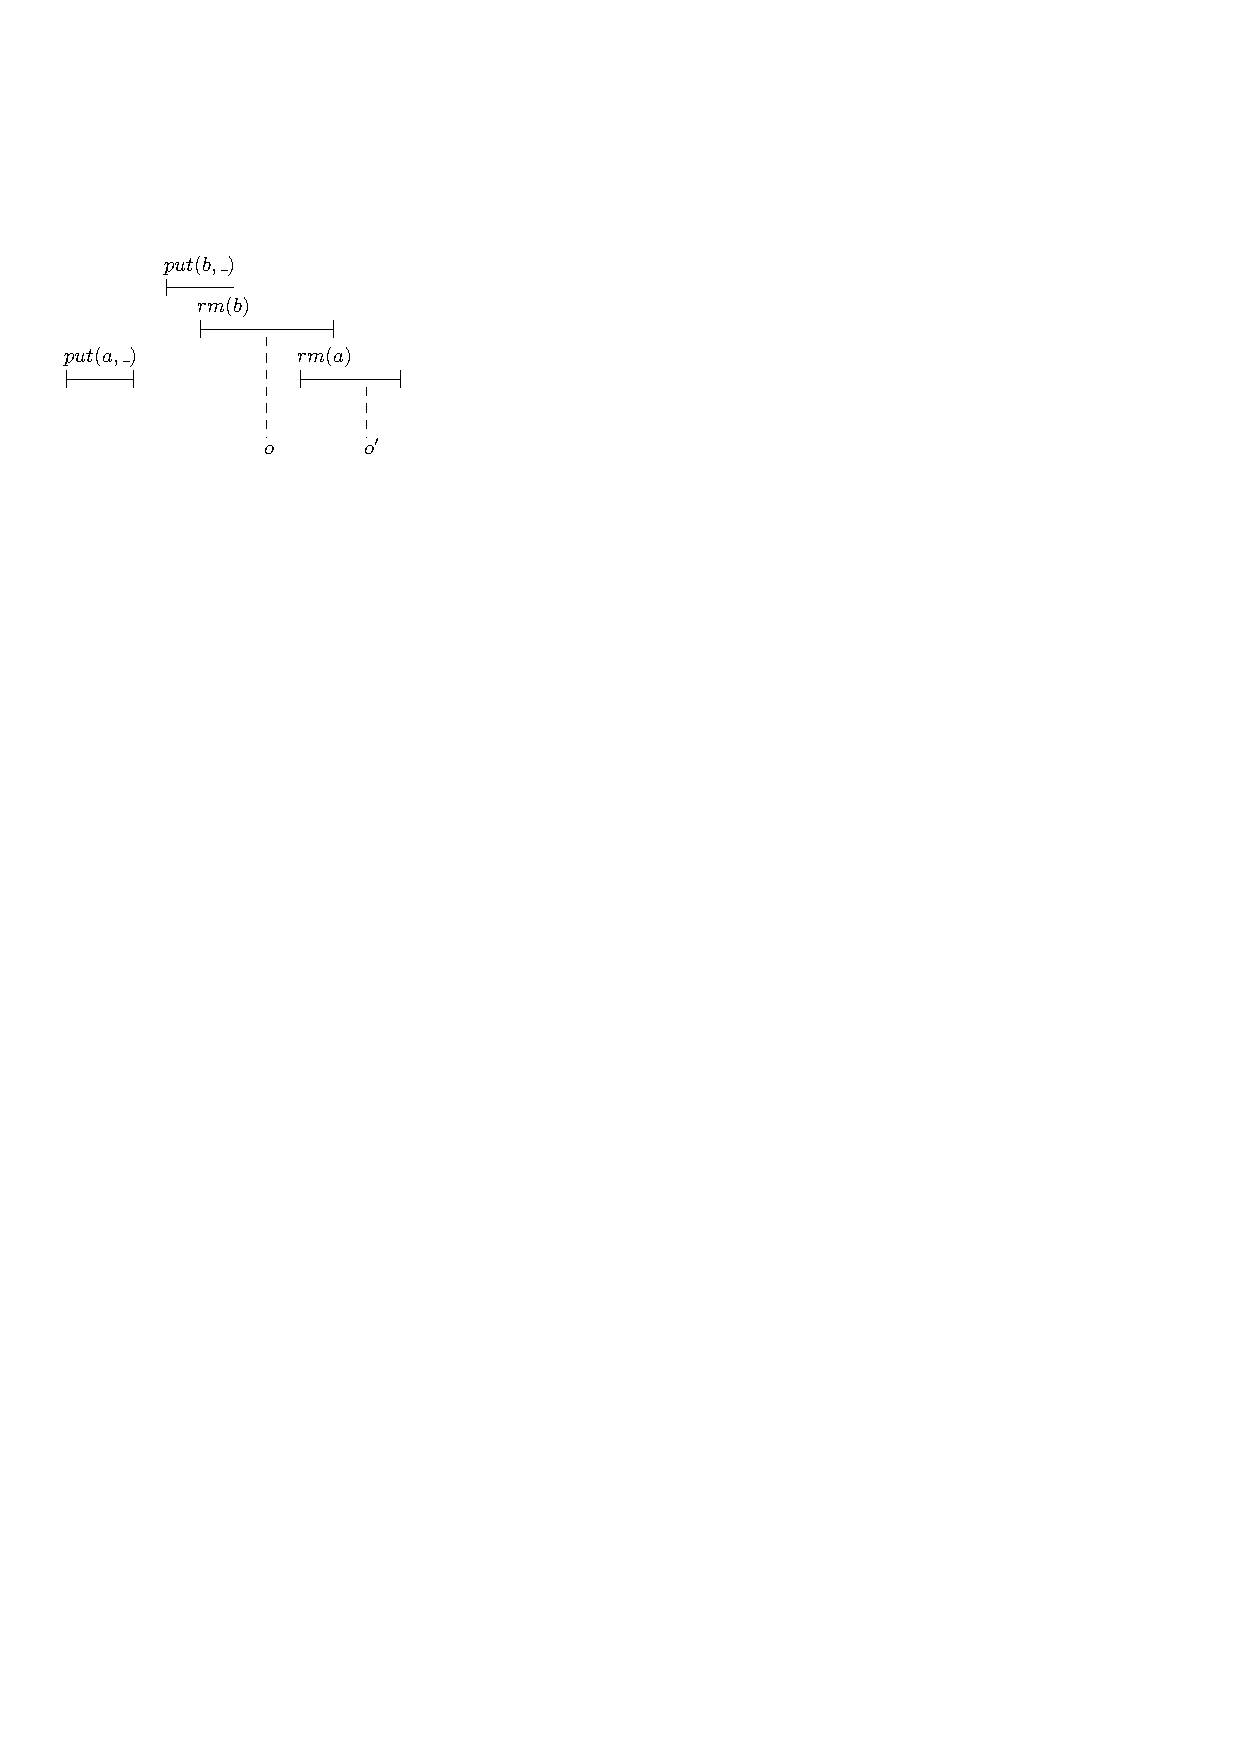
\includegraphics[width=0.4 \textwidth]{figures/PIC-HIS-PQ1Equal-1.pdf}
%\vspace{-10pt}
  \caption{The first possible enumeration.}
  \label{fig:history enumeration 1 for PQ1Equal}
\end{figure}


\begin{figure}[htbp]
  \centering
  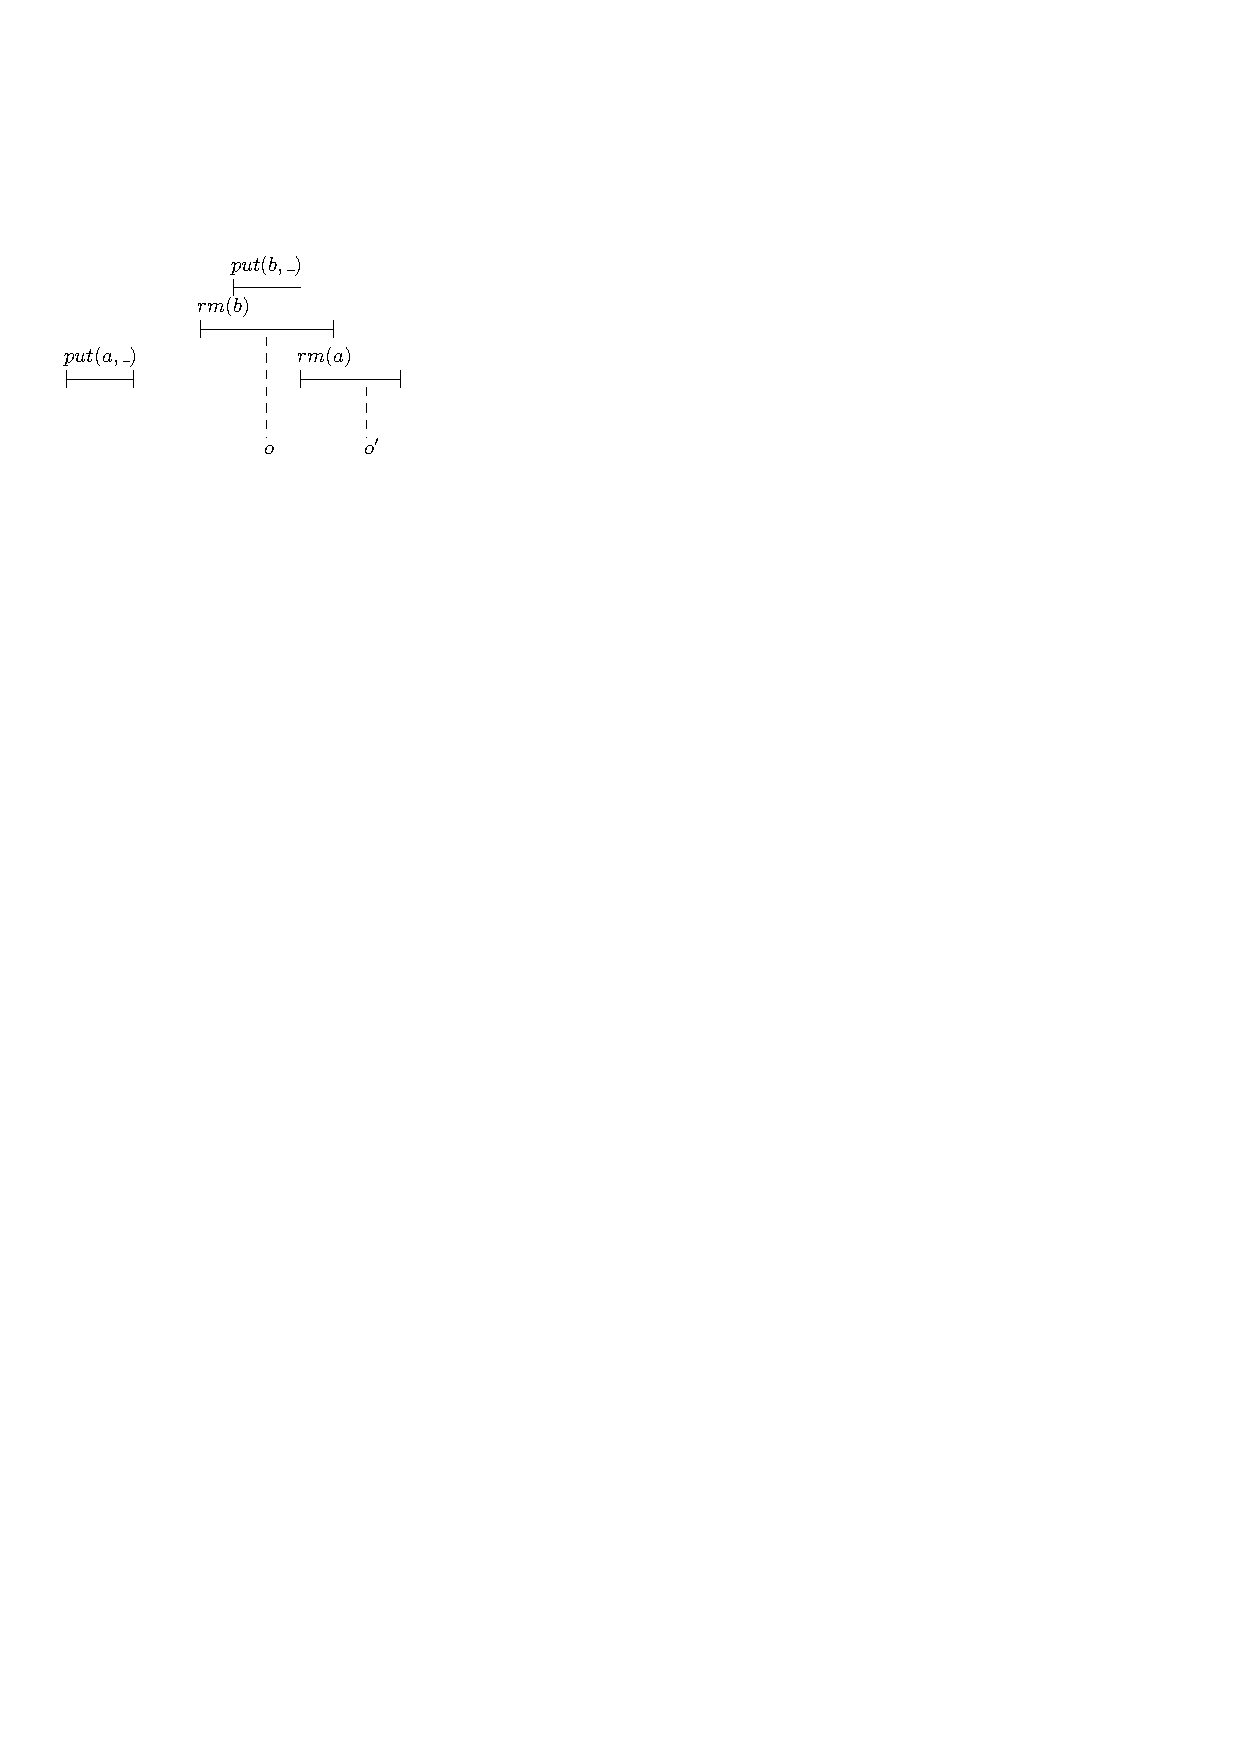
\includegraphics[width=0.4 \textwidth]{figures/PIC-HIS-PQ1Equal-2.pdf}
%\vspace{-10pt}
  \caption{The second possible enumeration.}
  \label{fig:history enumeration 2 for PQ1Equal}
\end{figure}

\begin{figure}[htbp]
  \centering
  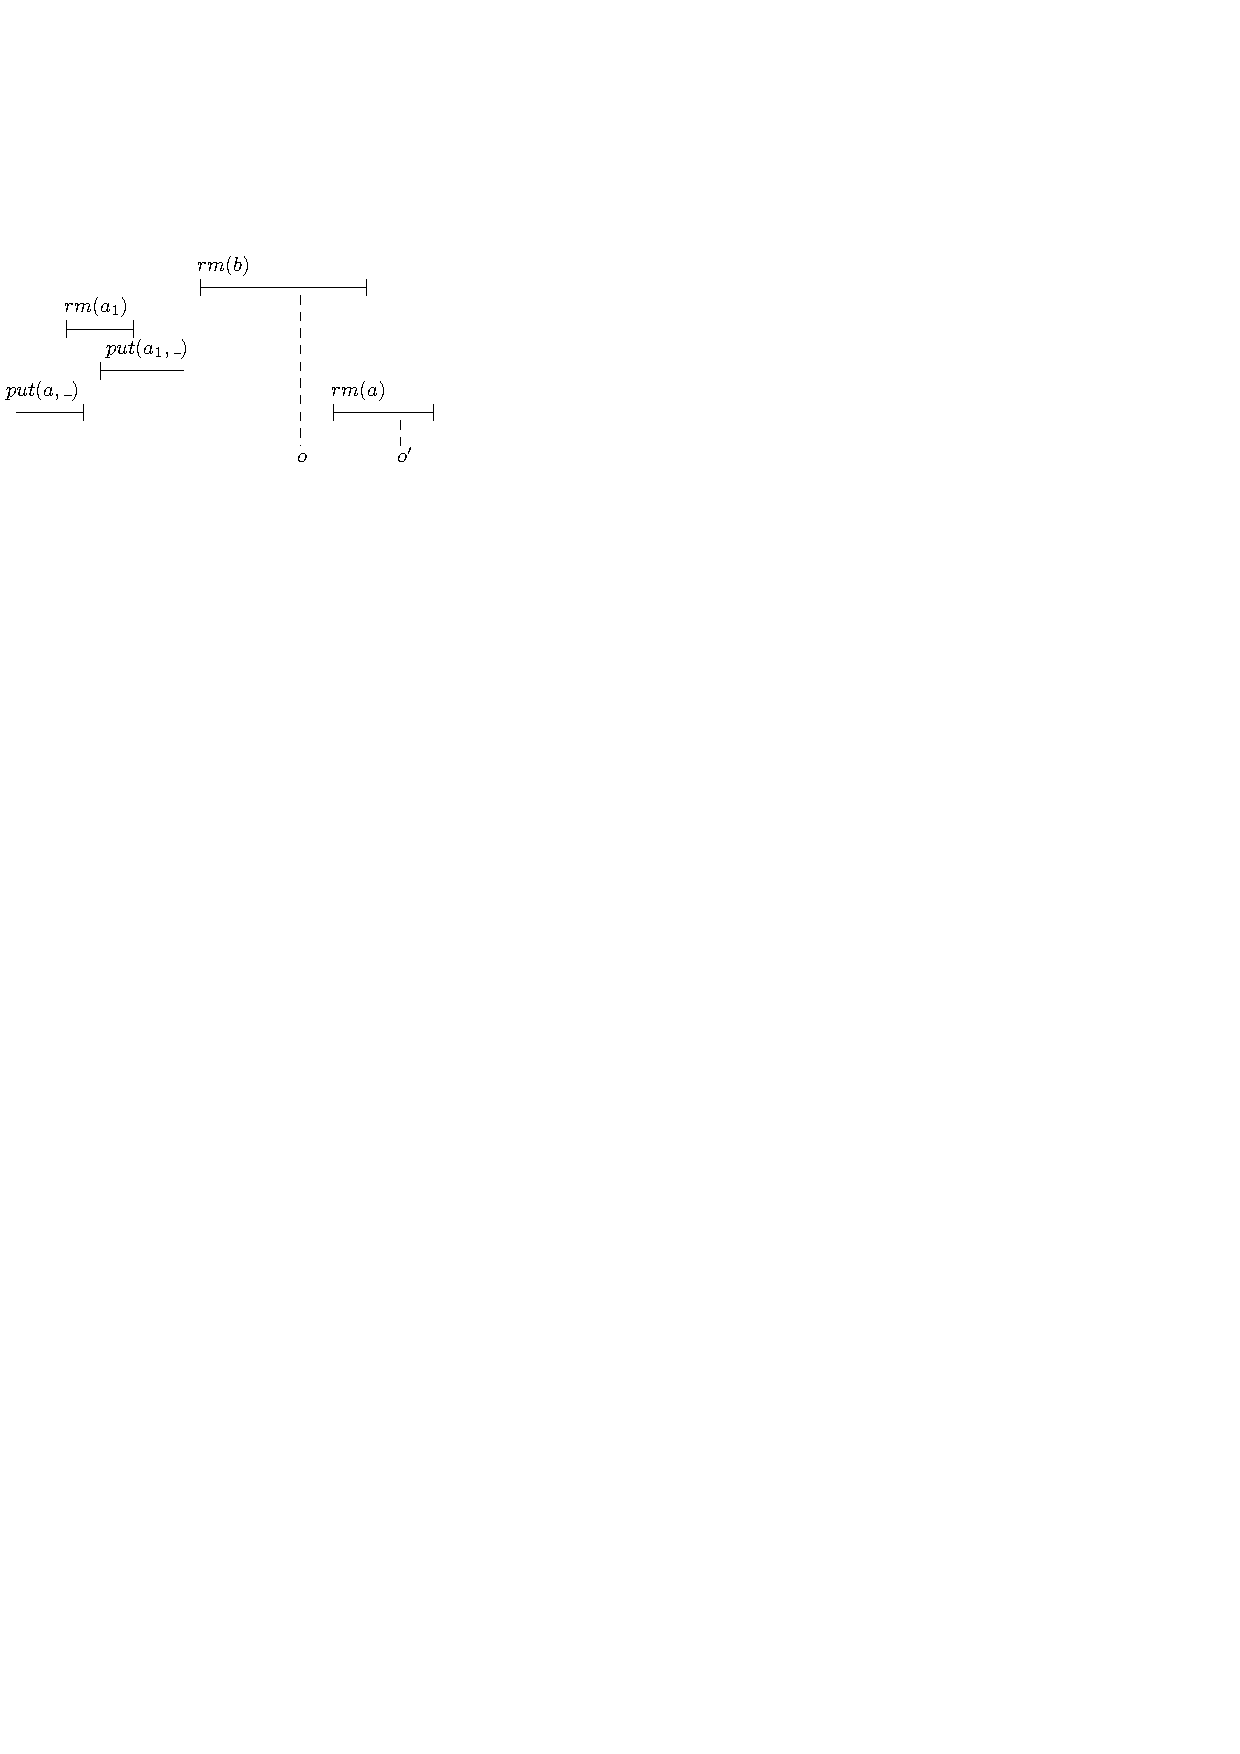
\includegraphics[width=0.4 \textwidth]{figures/PIC-HIS-PQ1Equal-3.pdf}
%\vspace{-10pt}
  \caption{The third possible enumeration.}
  \label{fig:history enumeration 3 for PQ1Equal}
\end{figure}

\begin{figure}[htbp]
  \centering
  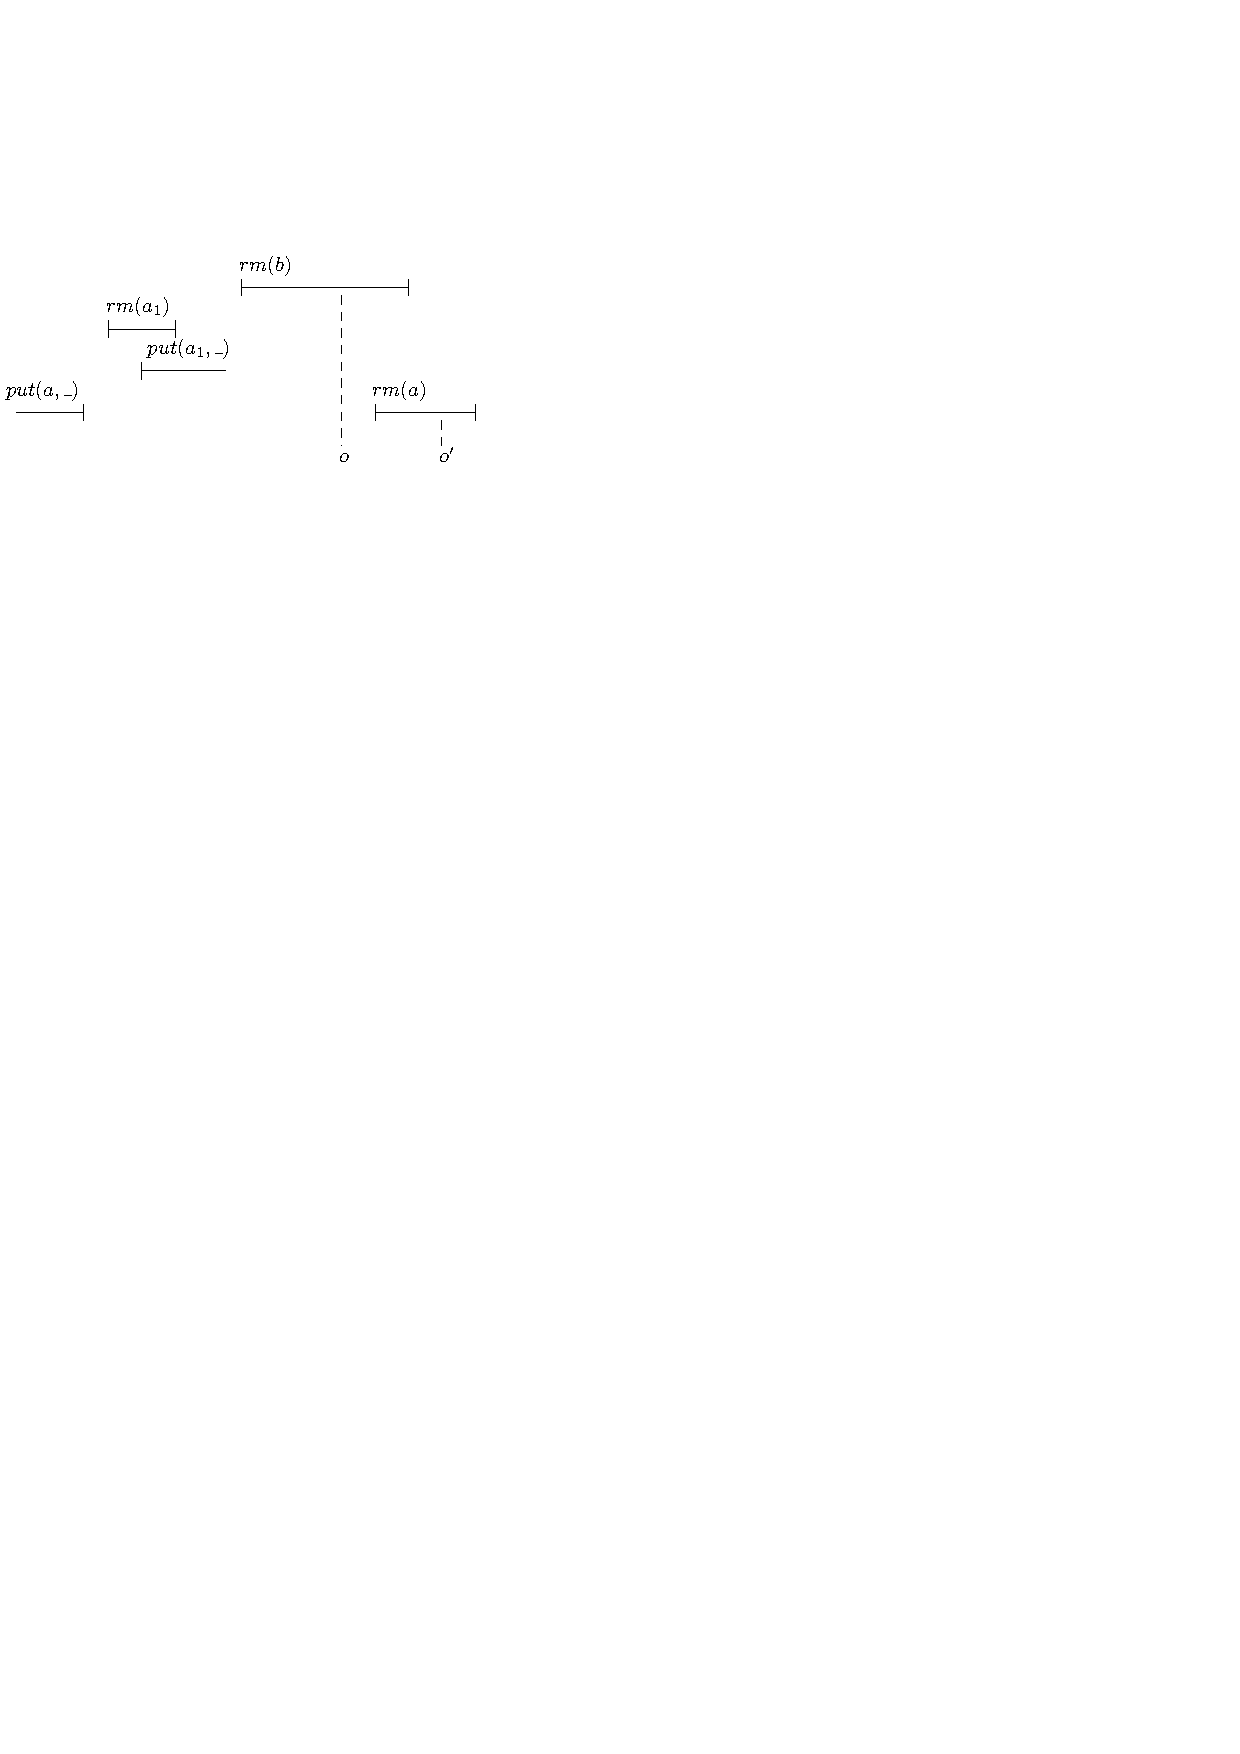
\includegraphics[width=0.4 \textwidth]{figures/PIC-HIS-PQ1Equal-4.pdf}
%\vspace{-10pt}
  \caption{The forth possible enumeration.}
  \label{fig:history enumeration 4 for PQ1Equal}
\end{figure}

\begin{figure}[htbp]
  \centering
  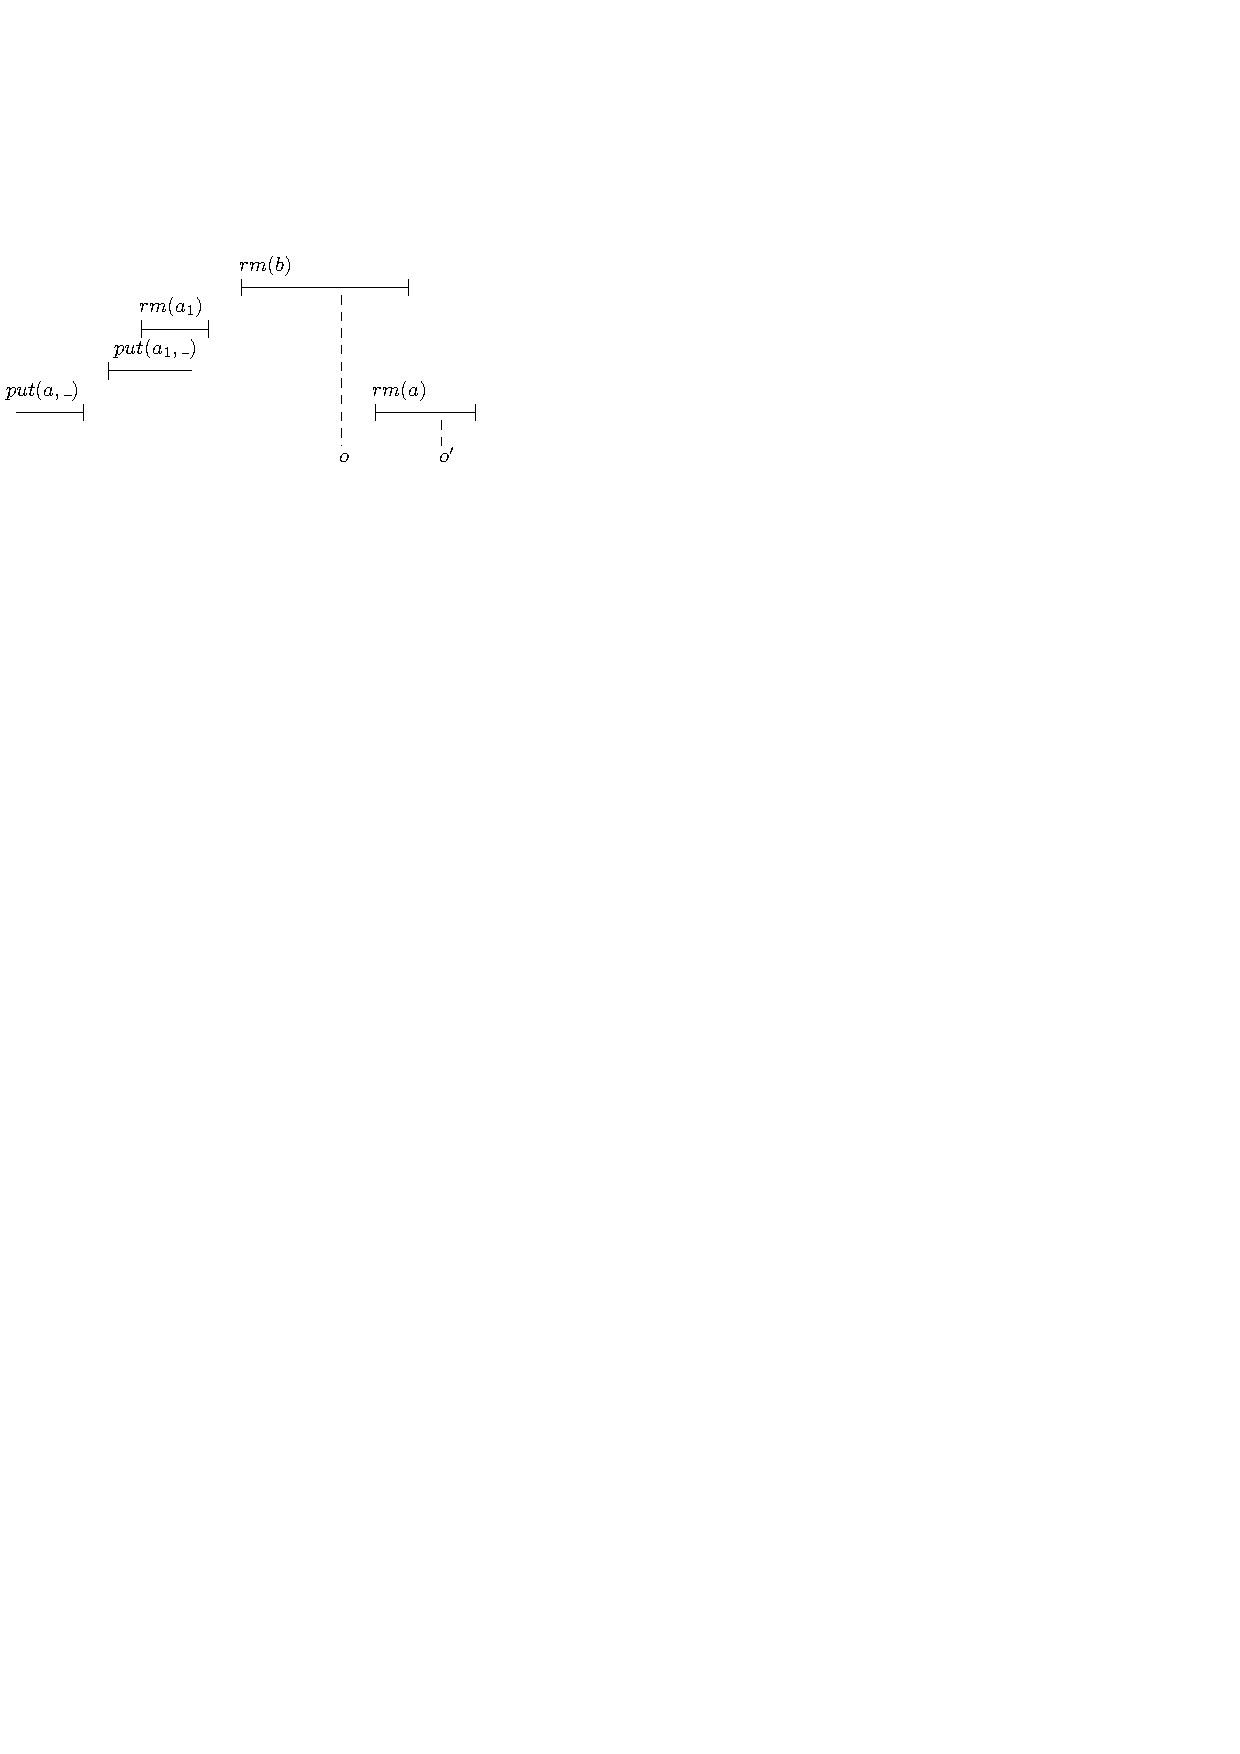
\includegraphics[width=0.4 \textwidth]{figures/PIC-HIS-PQ1Equal-5.pdf}
%\vspace{-10pt}
  \caption{The fifth possible enumeration.}
  \label{fig:history enumeration 5 for PQ1Equal}
\end{figure}


Let us begin to represent several witness automata that is used to capture the existence of a data-differentiated $\_$-execution $e$, $e$ has a projection $e'$, $\textit{last}(e') = \textit{EPQ}_1^{=}$, there exists items $a$ and $b$ with maximal priority in $e'$, $a <_{\textit{pb}}^* b$, and the rightmost gap-point of $b$ is before $\textit{cal}(\textit{put},a,\_)$ or $\textit{cal}(\textit{rm},a)$.

Given a data-differentiated $\_$-execution $e$, two actions $\textit{act}_1$, $\textit{act}_2$ of maximal priority in $e$, and assume that $\textit{act}_1$ is before $\textit{act}_2$ in $e$.
we say that $\textit{act}_1$, $\textit{act}_2$ is covered by items $d_1,\ldots,d_m$ in $e$, if the priorities of $d_1,\ldots,d_m$ is smaller than that of $\textit{act}_1$ and $\textit{act}_2$, and

\begin{itemize}
\setlength{\itemsep}{0.5pt}
\item[-] $\textit{ret}(\textit{put},d_m,\_)$ is before $\textit{act}_1$,

\item[-] For each $i < 1 \leq m$,$\textit{put}(d_{\textit{i-1}},\_)$ happens before $\textit{rm}(d_i)$,

\item[-] $\textit{act}_2$ is before $\textit{cal}(\textit{rm},d_1)$.
\end{itemize}

According to Lemma \ref{lemma:EPQ1Equal as pb order and gap-point}, Lemma \ref{lemma:ob order has bounded length} and Lemma \ref{lemma:five enumeration is enough for EPQ1Equal}, it is not hard to prove that, given a data-differentiated $\_$-execution $e$ with $\textit{last}(e) = \textit{EPQ}_1^{=}$, $e$ does not linearizable with respect to $\textit{EMS}(\textit{PQ}_1^{=})$, if and only if, one of enumerations holds in $e$ (permit renaming), while $\textit{cal}(\textit{rm},a)$ and $\textit{ret}(\textit{rm},b)$ is covered by some $d_1,\ldots,d_m$, $\textit{cal}(\textit{rm},b)$ is before $\textit{ret}(\textit{put},d_m,\_)$, and $\textit{cal}(\textit{rm},d_1)$ is before $\textit{ret}(\textit{rm},a)$. We say that such $d_1,\ldots,d_m$ constitute the rightmost gap of $b$.


An automaton $\mathcal{A}_{\textit{l-eq}}^1$ is given in \figurename~\ref{fig:automata for first enumeration of PQ1Equal}, and it is constructed for the first enumeration in \figurename~\ref{fig:history enumeration 1 for PQ1Equal}. Here we rename the items that covers $\textit{cal}(\textit{rm},a)$ and $\textit{ret}(\textit{rm},b)$ into $d$, and rename the remanning items into $e$. In this figure, $c = \textit{cal}(\textit{put},e,\textit{anyPri}),\textit{ret}(\textit{put},e)$, $\textit{cal}(\textit{rm},e), \textit{ret}(\textit{rm},e),\textit{cal}(\textit{rm},\textit{empty}),\textit{ret}(\textit{rm},\textit{empty})$, $c_1 = c + \textit{cal}(\textit{put},d,\textit{les}_p)$, $c_2 = c_1 + \textit{ret}(\textit{put},b)$, $c_3 = c_2 + \textit{cal}(\textit{put},d),\textit{ret}(\textit{rm},d)$, $c_4 = c + \textit{ret}(\textit{put},b) + \textit{ret}(\textit{rm},d)$.

\begin{figure}[htbp]
  \centering
  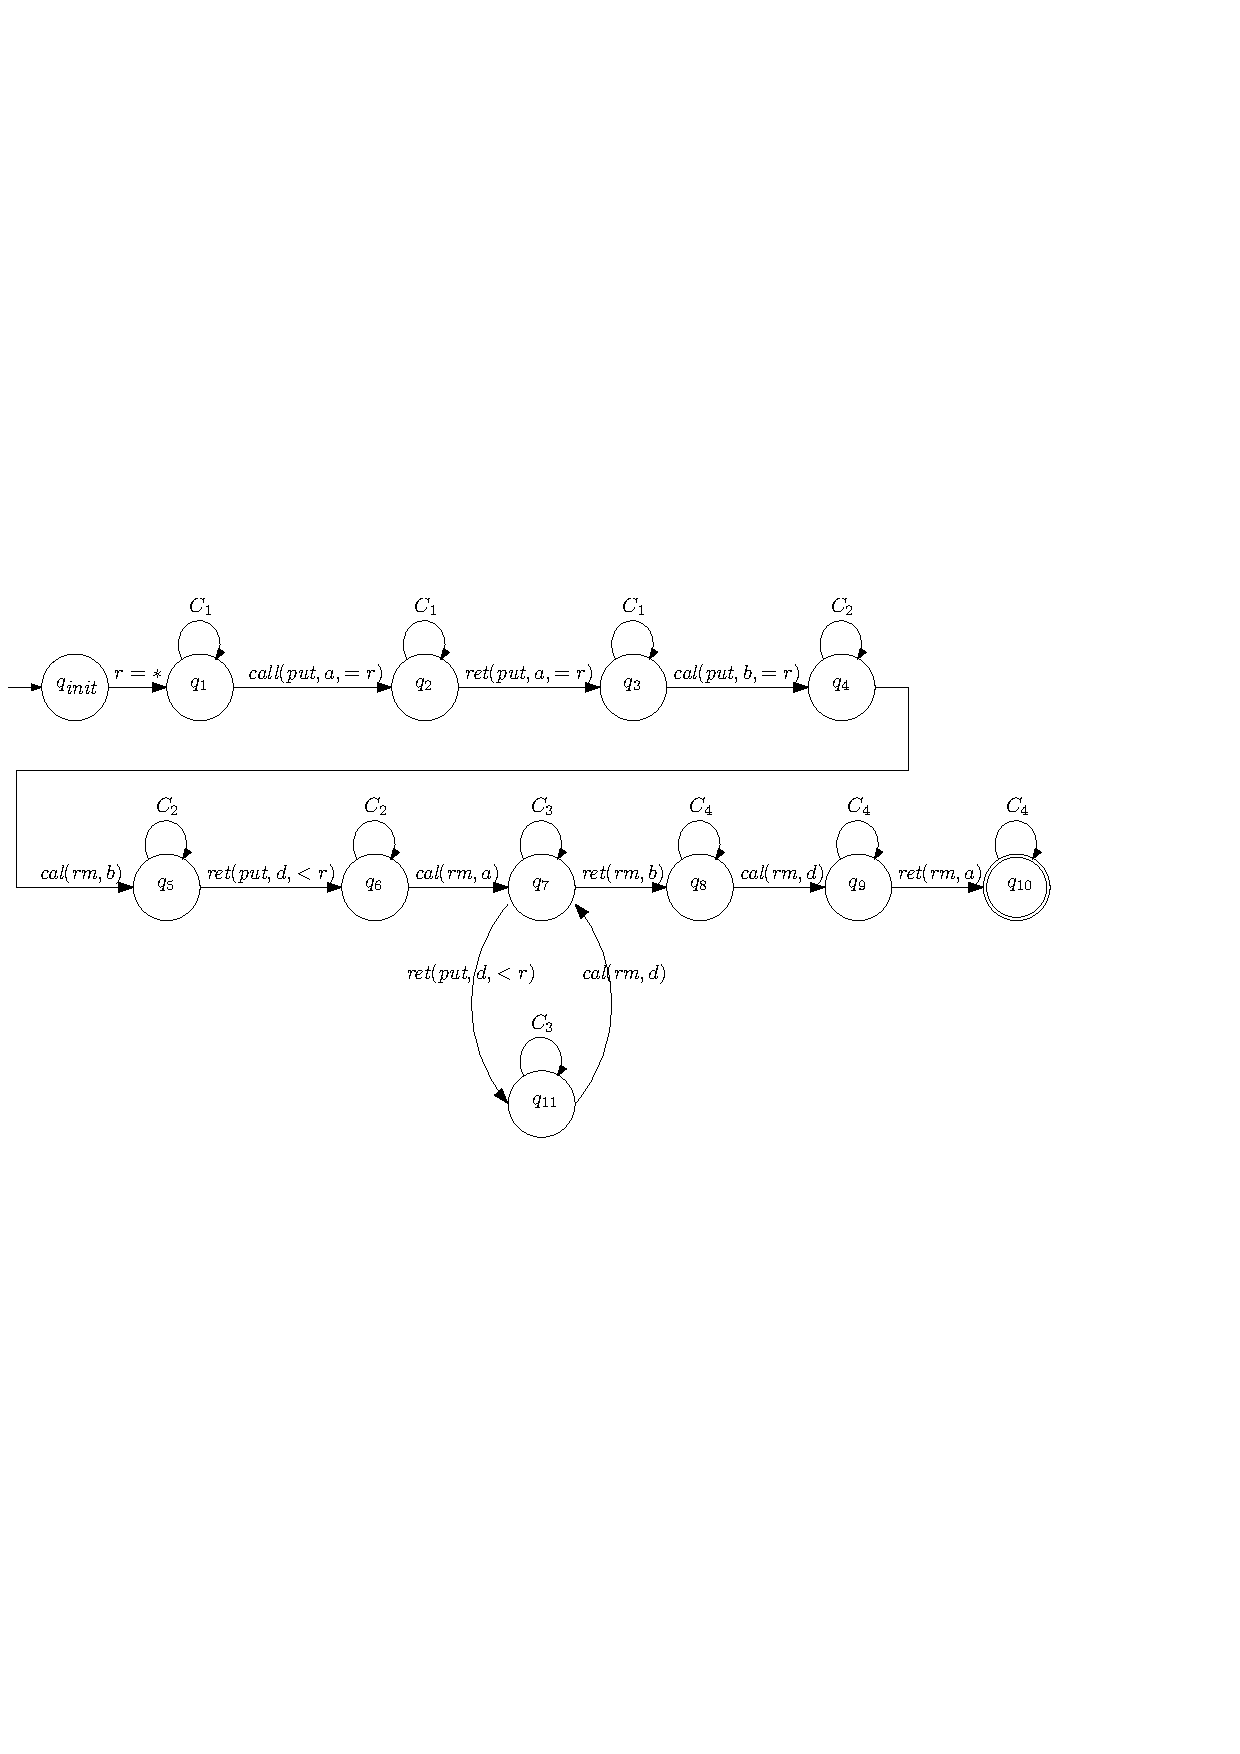
\includegraphics[width=0.8 \textwidth]{figures/PIC_AUTO_PQ1Equ-1.pdf}
%\vspace{-10pt}
  \caption{Automaton $\mathcal{A}_{\textit{l-eq}}^1$}
  \label{fig:automata for first enumeration of PQ1Equal}
\end{figure}


An automaton $\mathcal{A}_{\textit{l-eq}}^2$ is given in \figurename~\ref{fig:automata for second enumeration of PQ1Equal}, and it is constructed for the second enumeration in \figurename~\ref{fig:history enumeration 2 for PQ1Equal}. In \figurename~\ref{fig:automata for second enumeration of PQ1Equal}, $c_1$, $c_2$, $c_3$ and $c_4$ is same as that in \figurename~\ref{fig:automata for first enumeration of PQ1Equal}.

\begin{figure}[htbp]
  \centering
  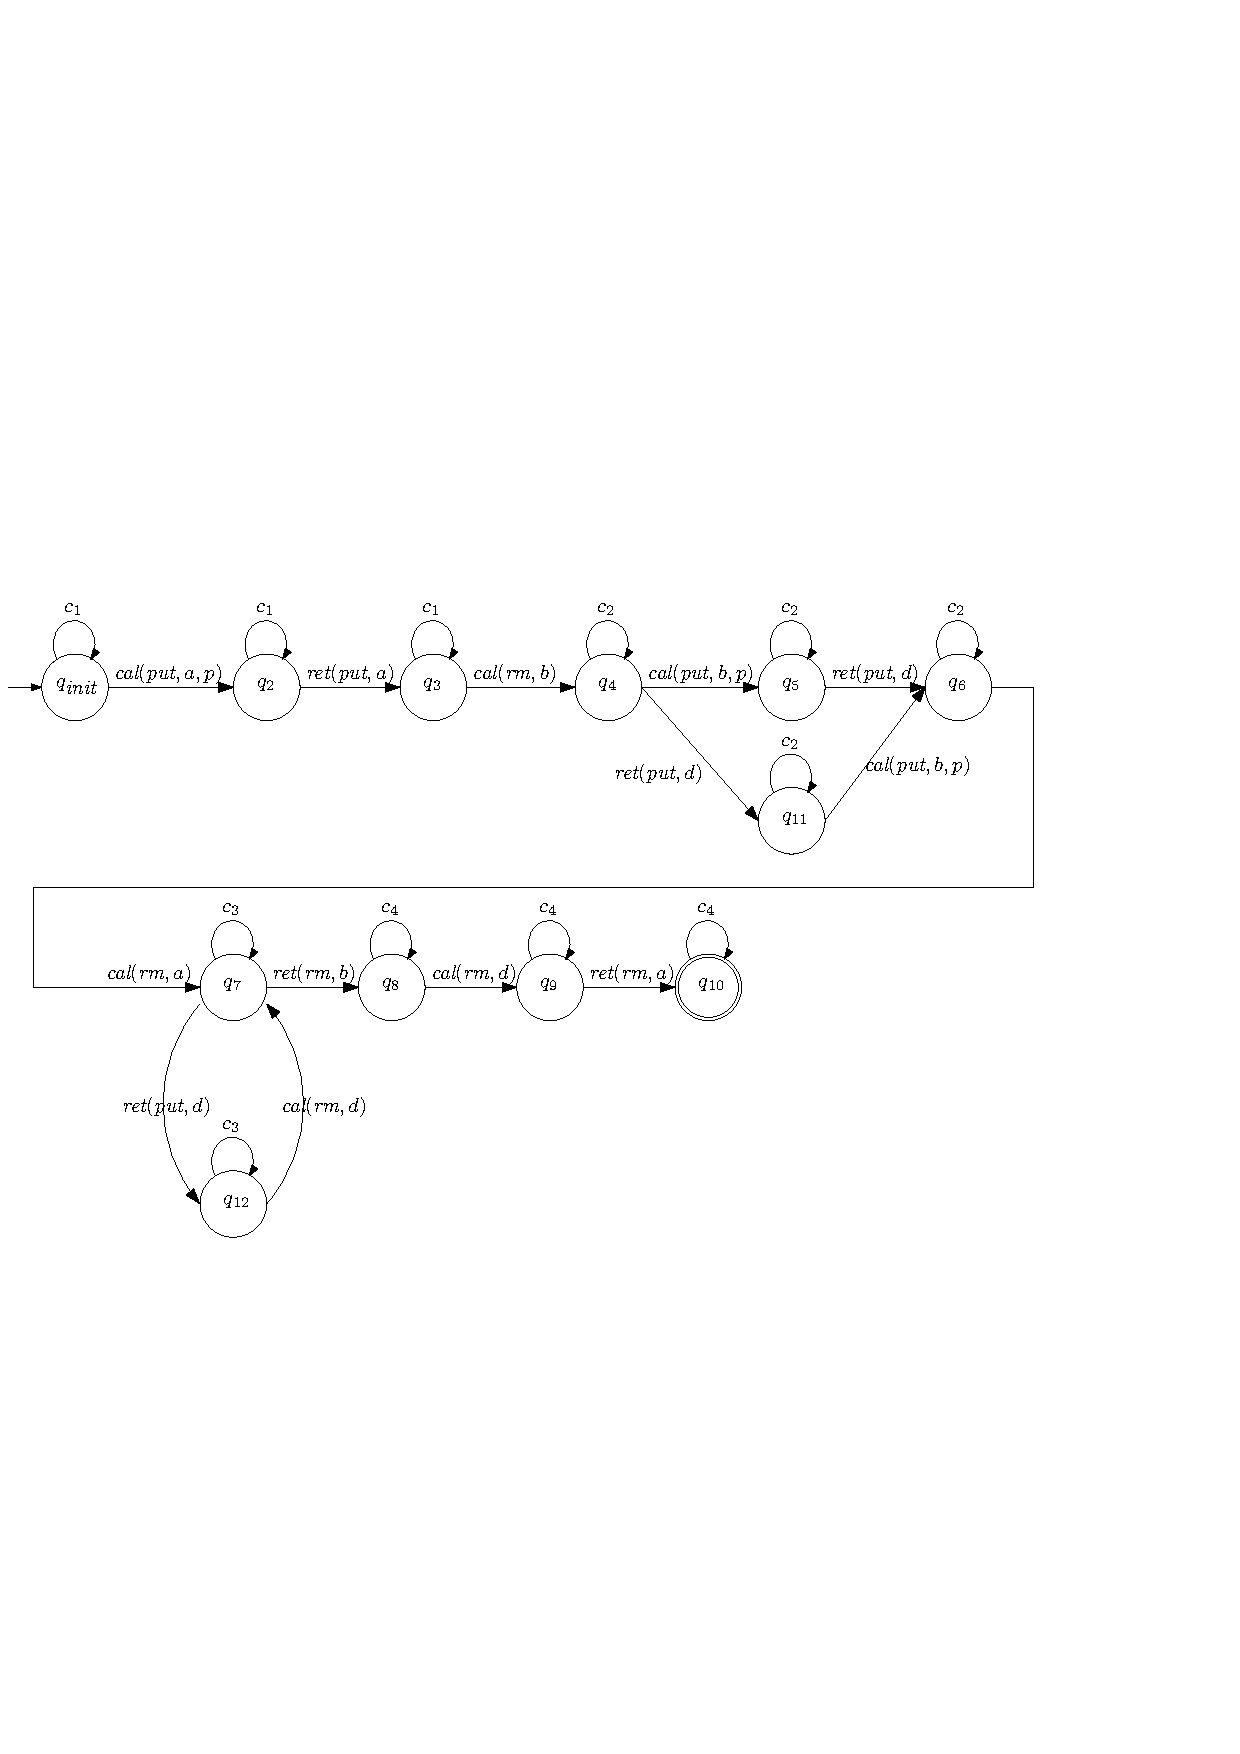
\includegraphics[width=0.8 \textwidth]{figures/PIC_AUTO_PQ1Equ-2.pdf}
%\vspace{-10pt}
  \caption{Automaton $\mathcal{A}_{\textit{l-eq}}^2$}
  \label{fig:automata for second enumeration of PQ1Equal}
\end{figure}

For the third enumeration in \figurename~\ref{fig:history enumeration 3 for PQ1Equal}. Since we want to ensure that $a$ and $b$ are putted only once, we need to explicitly record the positions of $\textit{cal}(\textit{put},a,p)$ and $\textit{cal}(\textit{put},b,p)$. Since the positions of $\textit{cal}(\textit{put},a,p)$ and $\textit{cal}(\textit{put},b,p)$ are not fixed, there are finite possible cases to consider, as shown below:

\begin{itemize}
\setlength{\itemsep}{0.5pt}
\item[-] If $\textit{cal}(\textit{put},b,p)$ is after $\textit{cal}(\textit{rm},b)$ and before $\textit{cal}(\textit{rm},a)$: There are two possible positions of $\textit{cal}(\textit{put},a,p)$: (1) before $\textit{cal}(\textit{rm},a_1)$, and (2) after $\textit{cal}(\textit{rm},a_1)$, and before $\textit{ret}(\textit{put},a)$.

\item[-] If $\textit{cal}(\textit{put},b,p)$ is after $\textit{ret}(\textit{rm},a_1)$ and before $\textit{cal}(\textit{rm},b)$: same as above case.

\item[-] If $\textit{cal}(\textit{put},b,p)$ is after $\textit{cal}(\textit{put},a_1,\_)$ and before $\textit{ret}(\textit{rm},a_1)$: same as above case.

\item[-] If $\textit{cal}(\textit{put},b,p)$ is after $\textit{ret}(\textit{put},a)$ and before $\textit{cal}(\textit{put},a_1,p)$: same as above case.

\item[-] If $\textit{cal}(\textit{put},b,p)$ is after $\textit{cal}(\textit{rm},a_1)$ and before $\textit{ret}(\textit{put},a)$: There are three possible positions of $\textit{cal}(\textit{put},a,p)$: (1) after $\textit{cal}(\textit{put},b,p)$ and before $\textit{ret}(\textit{put},a)$, (2) after $\textit{cal}(\textit{rm},a_1)$ and before $\textit{cal}(\textit{put},b,p)$, and (3) before $\textit{call}(\textit{rm},a_1)$.

\item[-] If $\textit{cal}(\textit{put},b,p)$ is before $\textit{cal}(\textit{rm},a_1)$: There are three possible positions of $\textit{cal}(\textit{put},a,p)$: (1) after $\textit{cal}(\textit{rm},a_1)$ and before $\textit{ret}(\textit{put},a)$, (2) after $\textit{cal}(\textit{put},b,p)$ and before $\textit{cal}(\textit{rm},a_1)$, and (3) before $\textit{cal}(\textit{put},b,p)$.
\end{itemize}

Therefore, there are fourteen possible cases that satisfy the third enumeration in \figurename~\ref{fig:history enumeration 3 for PQ1Equal}. For each case, we construct an finite automaton. Let $\textit{Auts}_{\textit{1-eq}}^{3}$ be the set of finite automata that is constructed for above fourteen cases. For example, for the case $\textit{ca}_1$ when $\textit{cal}(\textit{put},a,p)$ is before $\textit{cal}(\textit{rm},a_1)$, $\textit{cal}(\textit{put},b,p)$ is after $\textit{ret}(\textit{rm},a_1)$, and $\textit{cal}(\textit{put},b,p)$ is before $\textit{cal}(\textit{rm},b)$, we construct a finite automaton $\mathcal{A}_{\textit{l-eq}}^{\textit{3-1}}$ in \figurename~\ref{fig:automata for ca1 of third enumeration of Rpr2}. In \figurename~\ref{fig:automata for ca1 of third enumeration of Rpr2}, let $c$ and $c_1 = c + \textit{cal}(\textit{put},d,\textit{les}_p)$ the same as that in \figurename~\ref{fig:automata for first enumeration of PQ1Equal}. Let $c_2 = c_1 + \textit{ret}(\textit{put},a_1)$, $c_3 = c_2 + \textit{ret}(\textit{put},b)$, $c_4 = c_3 + \textit{cal}(\textit{put},d) + \textit{ret}(\textit{rm},d)$, and $c_5 = c + \textit{ret}(\textit{put},b) + \textit{ret}(\textit{put},a_1) + \textit{ret}(\textit{rm},d)$. The other witness automata in $\textit{Auts}_{\textit{1-eq}}^{3}$ can be similarly constructed.

\begin{figure}[htbp]
  \centering
  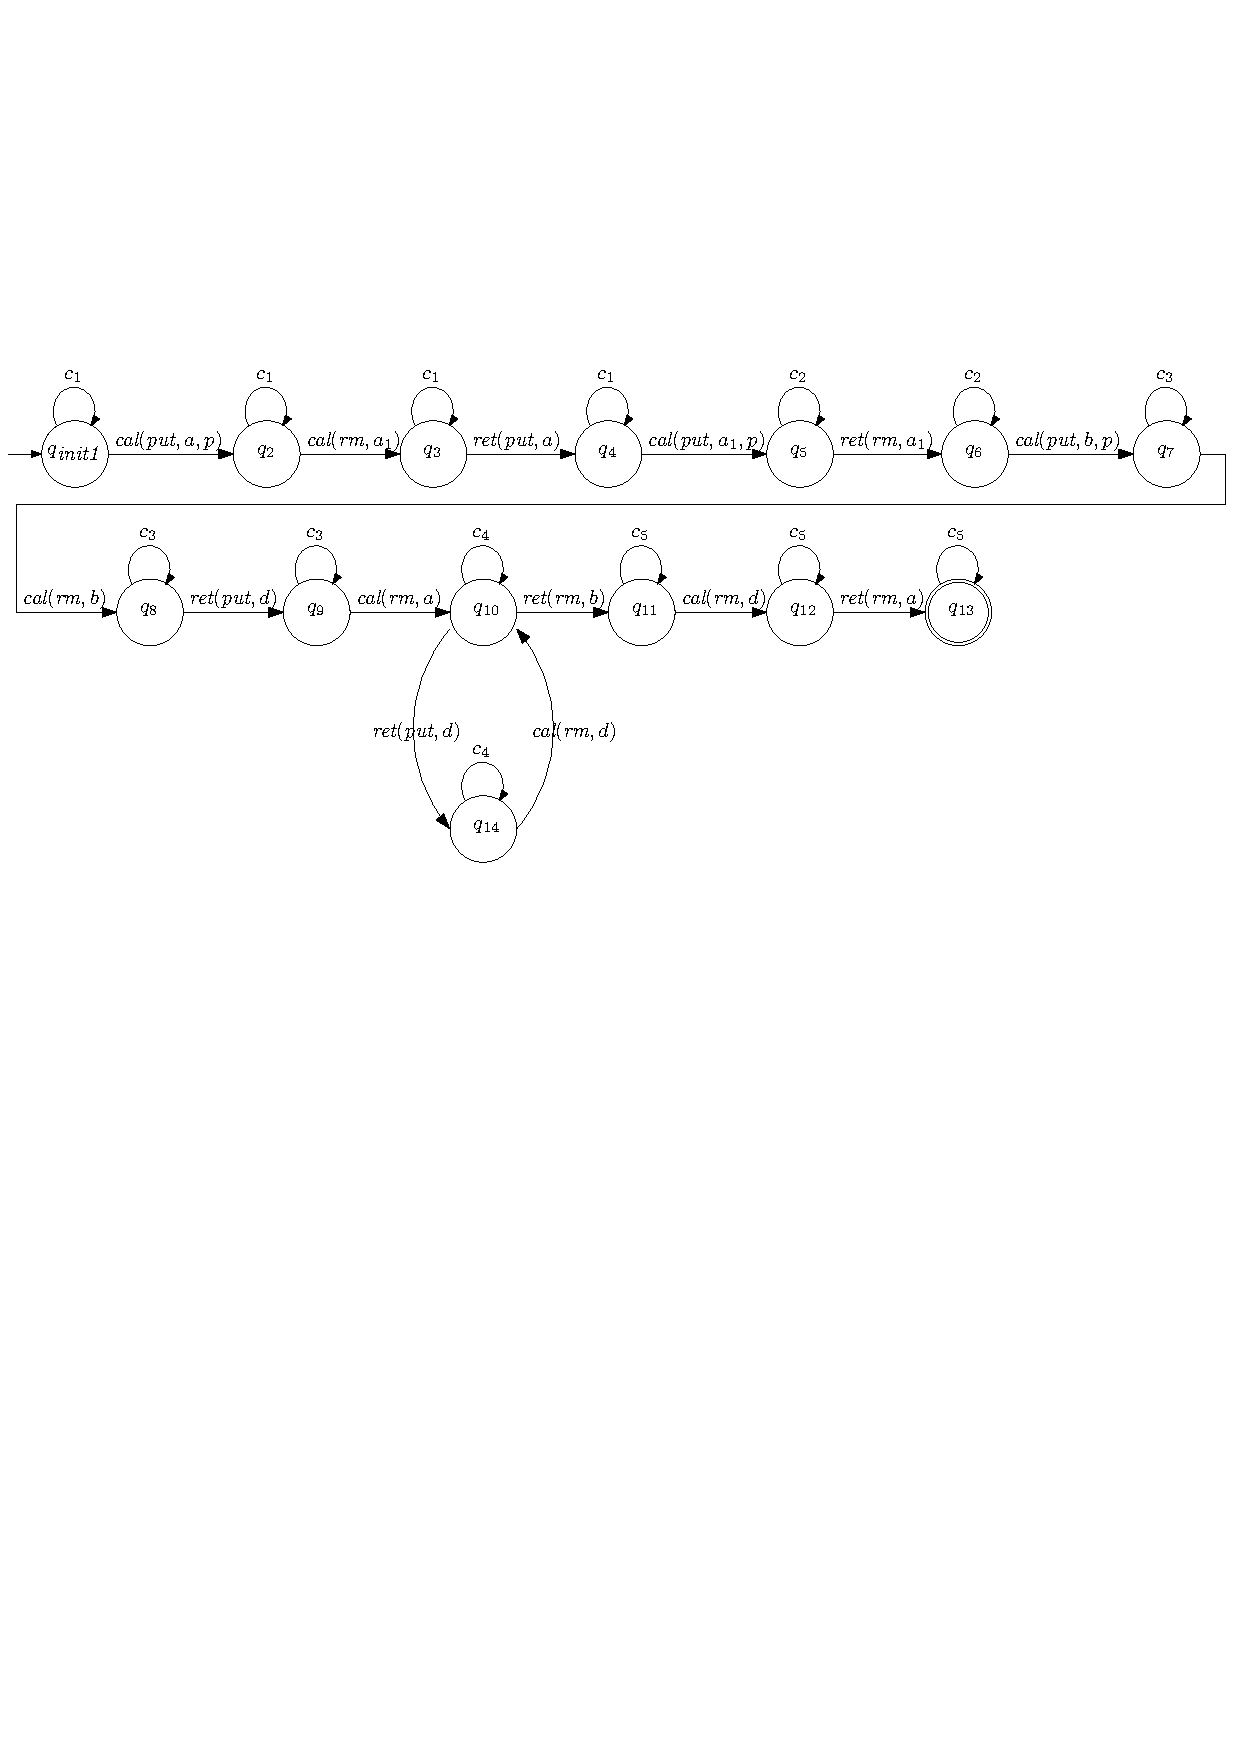
\includegraphics[width=0.8 \textwidth]{figures/PIC_AUTO_PQ1Equ-3-1.pdf}
%\vspace{-10pt}
  \caption{Automaton $\mathcal{A}_{\textit{l-eq}}^{\textit{3-1}}$}
  \label{fig:automata for ca1 of third enumeration of Rpr2}
\end{figure}

Similarly, we construct sets $\textit{Auts}_{\textit{1-eq}}^{4}$ and $\textit{Auts}_{\textit{1-eq}}^{5}$ of witness automata for the forth enumeration in \figurename~\ref{fig:history enumeration 4 for PQ1Equal} and the fifth enumeration in \figurename~\ref{fig:history enumeration 5 for PQ1Equal}, respectively.

Let $\textit{Auts}_{\textit{1-eq}} = \{ \mathcal{A}_{\textit{l-eq}}^1, \mathcal{A}_{\textit{l-eq}}^2 \} \cup \textit{Auts}_{\textit{1-eq}}^{3} \cup \textit{Auts}_{\textit{1-eq}}^{4} \cup \textit{Auts}_{\textit{1-eq}}^{5}$. The following lemma states that $\textit{PQ}_1^{=}$ is co-regular.


\EPQOneEqualIsCoRegular*

\begin {proof}

We need to prove that, given a data-independence implementation $\mathcal{I}$, $\textit{Auts}_{\textit{1-eq}} \cap \mathcal{I} \neq \emptyset$, if and only if $\exists e \in \mathcal{I}_{\neq},$ $e' \in \textit{proj}(e),$ $\textit{EPQ}_1^{=} \in \textit{last}(e') \wedge e'$ does not linearizable w.r.t. $\textit{MS}(\textit{EPQ}_1^{=})$.

By Lemma \ref{lemma:pri execution is enough} and Lemma \ref{lemma:EPQ1Equal as pb order and gap-point}, we need to prove the following fact:

\noindent {\bf $\textit{fact}_1$}: Given a data-independence implementation $\mathcal{I}$, $\textit{Auts}_{\textit{1-eq}} \cap \mathcal{I} \neq \emptyset$ if and only if $\exists e \in \mathcal{I}_{\neq},$ $e' \in \textit{proj}(e)$, $\textit{last}(e')=\textit{EPQ}_1^{=}$, $a$ and $b$ are two items with maximal priority $\textit{pri}$ in $e'$, $e'$ is a $\textit{pri}$-execution, $a <_{\textit{pb}}^* b$ in $e'$, and the rightmost gap-point of $b$ is before $\textit{cal}(\textit{put},a,\textit{pri})$ or $\textit{cal}(\textit{rm},a)$ in $e'$.

\noindent The $\textit{only if}$ direction: Assume that $e_1 \in \mathcal{I}$ is accepted by some witness automata in $\textit{Auts}_{\textit{1-eq}}$. By data-independence, there exists data-differentiated execution $e_2 \in \mathcal{I}$ and a renaming function $r$, such that $e_1=r(e_2)$. Since $e_1$ is accepted by some witness automata in  $\textit{Auts}_{\textit{1-eq}}$, let $x$, $y$ and $z$ (if exists) be the items that are renamed into $b$, $a$ and $a_1$ (if exists) by $r$, respectively, and let $d_1,\ldots,d_m$ be the items that are renamed into $d$ by $r$.

let $e'' = e_2 \vert_{ \{ x,y,z,d_1,\ldots,d_m \} }$. It is obvious that $e'' \in \textit{proj}(e_2)$ is a $\textit{pri}$-execution, $\textit{last}(e'') = \textit{EPQ}_1^{=}$. According to our construction of automata in $\textit{Auts}_{\textit{1-eq}}$, it is not hard to see that $x$ and $y$ has maximal priority in $h_2$, $y <_{\textit{pb}}^* x$, and the rightmost gap-point of $x$ is before $\textit{cal}(\textit{put},y,\textit{pri})$ or $\textit{cal}(\textit{rm},y)$ in $e''$.

\noindent The $\textit{if}$ direction: Assume that there exists $e \in \mathcal{I}_{\neq},e' \in \textit{proj}(e)$, such that $last(e')=\textit{PQ}_1^{=}$, $a'$ and $b'$ are two items with maximal priority $\textit{pri}$ in $e'$, $e'$ is a $\textit{pri}$-execution, $a' <_{\textit{pb}}^* b'$ in $e'$, and the rightmost gap-point of $b'$ is before $\textit{cal}(\textit{put},a',\textit{pri})$ or $\textit{cal}(\textit{rm},a')$ in $e'$. By data-independence, we can obtain execution $e_1$ as follows: (1) rename $a'$ and $b'$ into $a$ and $b$, respectively, (2) for the items $d_1,\ldots,d_m$ that constitute the rightmost gap of $b'$, we rename them into $d$, (3) if $a' <_{\textit{pb}}^A a'_1 <_{\textit{pb}}^B b$, we rename $a'_1$ into $a_1$, and (4) rename the other items into $e$. It is easy to see that $\textit{last}(e_1) = \textit{EPQ}_1^{=}$, $a$ and $b$ has maximal priority in $e_1$, $a <_{\textit{pb}}^* b$ in $e_1$, and the rightmost gap-point of $b$ is before $\textit{cal}(\textit{put},a,\textit{pri})$ or $\textit{cal}(\textit{rm},a)$ in $e_1$. By Lemma \ref{lemma:five enumeration is enough for EPQ1Equal}, there are five possible enumeration of operations of $a$, $b$, $a_1$ (if exists). Then


\begin{itemize}
\setlength{\itemsep}{0.5pt}
\item[-] If $a <_{\textit{pb}}^* b$ because of the first enumeration, it is easy to see that $h_1$ is accepted by $\mathcal{A}_{\textit{l-eq}}^1$.

\item[-] If $a <_{\textit{pb}}^* b$ because of the second enumeration, it is easy to see that $h_1$ is accepted by $\mathcal{A}_{\textit{l-eq}}^2$.

\item[-] If $a <_{\textit{pb}}^* b$ because of the third enumeration, it is easy to see that $h_1$ is accepted by some witness automaton in $\textit{Auts}_{\textit{1-eq}}^{3}$.

\item[-] If $a <_{\textit{pb}}^* b$ because of the forth enumeration, it is easy to see that $h_1$ is accepted by some witness automaton in $\textit{Auts}_{\textit{1-eq}}^{4}$.

\item[-] If $a <_{\textit{pb}}^* b$ because of the fifth enumeration, it is easy to see that $h_1$ is accepted by some witness automaton in $\textit{Auts}_{\textit{1-eq}}^{5}$.
\end{itemize}

This completes the proof of this lemma. \qed
\end {proof}





\subsection{Co-Regular of $\textit{EPQ}_2^{>}$}
\label{subsec:appendix co-regular of EPQ2Lar}


\begin{restatable}{lemma}{EPQ2LarIsAlwaysCoRegular}
\label{lemma:EPQ2Lar is always co-regular}
Given a data-differentiated $\_$-execution $e$, if $\textit{last}(e) = \textit{EPQ}_2^{>}$, then $e \sqsubseteq \textit{MS}(\textit{EPQ}_2^{>})$.
\end{restatable}

\begin {proof}
Since $\textit{last}(e) = \textit{EPQ}_2^{>}$, the actions with maximal priority in $e$ is some unmatched $\textit{put}$. Therefore, no matter how we locate linearization points, we can always obtain a sequence $l$ of method events that contains unmatched $\textit{put}$ with maximal priority, and this satisfy the guard of $\textit{MS}(\textit{EPQ}_2^{>})$. This completes the proof of this lemma. \qed
\end {proof}




\subsection{Co-Regular of $\textit{EPQ}_2^{=}$}
\label{subsec:appendix co-regular of EPQ2Equal}

\begin{restatable}{lemma}{EPQ2EqualAsHappenBefore}
\label{lemma:EPQ2Equal as happen before}
Given a data-differentiated $\textit{pri}$-execution $e$ with $\textit{last}(e) = \textit{EPQ}_2^{=}$. $e$ does not linearizable to $\textit{MS}(\textit{EPQ}_2^{=})$, if and only if there exists $x$ and $y$ with priority $\textit{pri}$, $x$ has unmatched $\textit{put}$, $y$ has matched $\textit{put}$ and $\textit{rm}$, and $\textit{put}(x,\textit{pri}) <_{\textit{hb}} \textit{put}(y,\textit{pri})$.
\end{restatable}

\begin {proof}

The $\textit{if}$ direction is obvious.

To prove the $\textit{only if}$ direction, we prove its contrapositive. Assume that for each pair of $x$ and $y$ with maximal priority in $e$, if $x$ has unmatched $\textit{put}$, $y$ has matched $\textit{put}$ and $\textit{rm}$, then $\textit{put}(x,\textit{pri})$ does not happen before $\textit{put}(y,\textit{pri})$. We need to prove that $e \sqsubseteq \textit{MS}(\textit{EPQ}_2^{=})$.

Let $x_1,\ldots,x_m$ be the set of items with priority $\textit{pri}$ and has unmatched $\textit{put}$ in $e$, let $y_1,\ldots,y_n$ be the set of items with priority $\textit{pri}$ and has matched $\textit{put}$ and $\textit{rm}$ in $e$. By assumption, we know that $\textit{cal}(\textit{put},y_i,\textit{pri})$ is before $\textit{ret}(\textit{put},x_j)$ for each $i,j$. Then we explicitly construction the linearization of $e$ by locating the linearization points of $e$ as follows:

\begin{itemize}
\setlength{\itemsep}{0.5pt}
\item[-] For each $x_i$, locate the linearization point of $\textit{put}(x_i,\textit{pri})$ just before its return action.

\item[-] For each $y_j$, locate the lineariztion point of $\textit{put}(y_j,\textit{pri})$ jest after its call action.

\item[-] For other method events, locate their linearization points at an arbitrary location after its call action and before its return action.
\end{itemize}

Let $l$ be the sequence of linearization points. It is easy to see that $e \sqsubseteq l$. Since linearization points of $\textit{put}(x_i,\textit{pri})$ is after the linearization point of $\textit{put}(y_j,\textit{pri})$ for each $i,j$, it is easy to see that $l \in \textit{MS}(\textit{EPQ}_2^{=})$. This completes the proof of this lemma. \qed
\end {proof}

Lemma \ref{lemma:EPQ2Equal as happen before} shows how to check violation to $\textit{MS}(\textit{EPQ}_2^{=})$. However, the case in Lemma \ref{lemma:EPQ2Equal as happen before} violates our assumption that each single-priority execution is FIFO. Therefore, we know that $\textit{EPQ}_2^{=}$ is always co-regular, as states by the following lemma.

\begin{restatable}{lemma}{EPQ2EqualIsAlwaysCoRegular}
\label{lemma:EPQ2Equal is always co-regular}
Given a data-differentiated $\textit{pri}$-execution $e$, if $\textit{last}(e) = \textit{EPQ}_2^{=}$, then $e \sqsubseteq \textit{MS}(\textit{EPQ}_2^{=})$.
\end{restatable}

\begin {proof}

According to Lemma \ref{lemma:EPQ2Equal as happen before}, if $\textit{last}(e) = \textit{EPQ}_2^{=}$ and $e$ does not linearizable to $\textit{MS}(\textit{EPQ}_2^{=})$, then there exists $x$ and $y$ with priority $\textit{pri}$, $x$ has unmatched $\textit{put}$, $y$ has matched $\textit{put}$, and $\textit{put}(x,\textit{pri}) <_{\textit{hb}} \textit{put}(y,\textit{pri})$. Let $e_1 = e \vert_{ \{ x,y \} }$. It is obvious that $e_1$ does not satisfy FIFO property. This contradicts the assumption that every single-priority execution has FIFO property, and thus, we can safely ignore this case. \qed
\end {proof}




\subsection{Co-Regular of $\textit{EPQ}_3$}
\label{subsec:co-regular of EPQ3}

In this subsection we prove that $\textit{EPQ}_3$ is co-regular. The notion of left-right constraint of $\textit{rm}(\textit{empty})$ is inspired by left-right constraint of queue \cite{Bouajjani:2015}.

\begin{definition}\label{def:left-right constraint for rmEmpty operation}
Given a data-differentiated execution $e$, and $o = \textit{rm}(\textit{empty})$ of $e$. The left-right constraint of $o$ is the graph $G$ where:

\begin{itemize}
\setlength{\itemsep}{0.5pt}
\item[-] the nodes are the items of $e$ or $o$, to which we add a node,

\item[-] there is an edge from item $d_1$ to $o$, if $\textit{put}(d_1,\_)$ happens before $o$,

\item[-] there is an edge from $o$ to item $d_1$, if $o$ happens before $\textit{rm}(d_1)$ or $\textit{rm}(d_1)$ does not exists in $h$,

\item[-] there is an edge from item $d_1$ to item $d_2$, if $\textit{put}(d_1,\_)$ happens before $\textit{rm}(d_2,\_)$.
\end{itemize}
\end{definition}


Given a data-differentiated execution $e$ and $o = \textit{rm}(\textit{empty})$ of $e$, it is obvious that $\textit{last}(e) = \textit{EPQ}_3$. Let $\textit{USet}_1(e,o) = \{ \textit{op} \vert$ $\textit{op}$ is an operation of some item, and either $\textit{op} <_{\textit{hb}} o$, or there is $\textit{op}'$ with the same item of $\textit{op}$, such that $\textit{op}' <_{\textit{hb}} o \}$. For each $i \geq 1$, let $\textit{USet}_{\textit{i+1}}(e,o) = \{ \textit{op} \vert$ $\textit{op}$ is an operation of some item, $\textit{op}$ is not in $\textit{USet}_k(e,o)$ for each $k \leq i$, and either $\textit{op}$ happens before some $o' \in \textit{USet}_i(e,o)$, or there is $\textit{op}''$ with the same item of $o$ and $\textit{op}''$ happens before some $o' \in \textit{USet}_i(e,o) \}$. We can see that $\textit{USet}_i(e,o) \cap \textit{USet}_j(e,o) = \emptyset$ for any $i \neq j$. Let $\textit{USet}(e,o) = \textit{USet}_1(e,o) \cup \textit{USet}_2(e,o) \cup \ldots$.


Similarly as $\textit{UVSet}$, we can prove the following two lemmas for $\textit{USet}$.

\begin{restatable}{lemma}{USetHasMatchedPutandRm}
\label{lemma:USet has matched put and rm}
Given a data-differentiated execution $e$ with $\textit{last}(e) = \textit{EPQ}_3$. Let $o$ be a $\textit{rm}(\textit{empty})$ of $e$. Let $G$ be the graph representing the left-right constraint of $o$. Assume that $G$ has no cycle going through $o$. Then, $\textit{USet}(e,o)$ contains only matched $\textit{put}$ and $\textit{rm}$.
\end{restatable}

This Lemma can be similarly proved as Lemma \ref{lemma:UVSet has matched put and rm}.


\begin{restatable}{lemma}{RmxDoesNotHappenBeforeUSetForEPQ3}
\label{lemma:Rmx does not happen before USet for EPQ3}
Given a data-differentiated $\_$execution $e$ with $\textit{last}(e) = \textit{EPQ}_3$. Let $o$ be a $\textit{rm}(\textit{empty})$ of $e$. Let $G$ be the graph representing the left-right constraint of $o$. Assume that $G$ has no cycle going through $o$. Then, $o$ does not happen before any operation in $\textit{USet}(e,o)$.
\end{restatable}

This Lemma can be similarly proved as Lemma \ref{lemma:Rmx does not happen before UVSet for EPQ1Lar}.

Then we can prove that getting rid of cycle though $o$ in left-right constraint is enough for ensure linearizable w.r.t $\textit{MS}(\textit{EPQ}_3)$, as stated by the following lemma.


\begin{restatable}{lemma}{LINEqualsConstraintforEPQ3}
\label{lemma:Lin Equals Constraint for EPQ3}
Given a data-differentiated execution $e$ with $\textit{last}(e) = \textit{EPQ}_3$. $e$ does not linearizable w.r.t $\textit{MS}(\textit{PQ}_3)$, if and only if there exists $o = \textit{rm}(\textit{empty})$ in $e$, $G$ has a cycle going through $o$, where $G$ is the graph representing the left-right constraint of $o$.
\end{restatable}

\begin {proof}

To prove the $\textit{if}$ direction, assume that there is such a cycle. Assume by contradiction that $e \sqsubseteq \textit{MS}(\textit{EPQ}_3)$, and let $U$ and $V$ be the set of operations in $u$ and $v$. Let the cycle be $d_1 \rightarrow d_2 \rightarrow \ldots \rightarrow d_m \rightarrow o \rightarrow d_1$ in $G$. Since $d_m \rightarrow o$, $\textit{put}(d_m,\_)$ happens before $o$, and it is easy to see that $\textit{put}(d_m,\_)$ is in $U$. Since $U$ contains matched $\textit{put}$ and $\textit{rm}$, we can see that operations of $d_m$ is in $U$. Similarly, we can see that method events of $d_{\textit{m-1}},\ldots,d_1$ is in $U$. If $\textit{rm}(d_1)$ does not exists, then this contradicts that $U$ contains matched $\textit{put}$ and $\textit{rm}$. Else, if $\textit{rm}(d_1)$ exists, since $o$ happens before $\textit{rm}(d_1)$, we can see that $\textit{rm}(d_1) \in V$, which contradicts that $\textit{rm}(d_1) \in U$. This completes the proof of the $\textit{if}$ direction.

To prove the $\textit{only if}$ direction, we prove its contrapositive. Assume that for each such $o$ and $G$, $G$ has no cycle going through $o$. Let $O$ be the set of operations of $e$, except for $\textit{rm}(\textit{empty})$. Let $O_L = \textit{USet}(e,o)$, $O_R = O \setminus O_L$.

By Lemma \ref{lemma:USet has matched put and rm}, we can see that $O_L = \textit{USet}(e,o)$ contains only matched $\textit{put}$ and $\textit{rm}$. Let $O'_L$ be the union of $O_L$ and all the $\textit{rm}(\textit{empty})$ that happens before some operations in $O_L \cup \{ o \}$. Let $O'_R$ be the union of $O_R$ and the remanning $\textit{rm}(\textit{empty})$. It remains to prove that for $O'_L$, $\{ o \}$, $O'_R$, no elements of the latter set happens before elements of the former set. We prove this by showing that all the following cases are impossible:

\begin{itemize}
\setlength{\itemsep}{0.5pt}
\item[-] Case $1$: If some operation $o_r \in O'_R$ happens before $o$. Then we can see that $o_r \in \textit{USet}(e,o)$ or is a $\textit{rm}(\textit{empty})$ that happens before $o$, and then $o_r \in O'_L$, which contradicts that $o_r \in O'_R$.

\item[-] Case $2$: If some operation $o_r \in O'_R$ happens before some operation $o_l \in O'_L$. Then we know that $o_r \in \textit{USet}(e,o)$ or is a $\textit{rm}(\textit{empty})$ that happens before some operations in $O_L \cup \{ o \}$, and then $o_r \in O'_L$, which contradicts that $o_r \in O'_R$.

\item[-] Case $3$: If $o$ happens before some $o_l \in O'_L$. If $o_l \in \textit{USet}(e,o)$, then by Lemma \ref{lemma:Rmx does not happen before USet for EPQ3} we know that this is impossible. Else, $o_l$ is a $\textit{rm}(\textit{empty})$ that happens before some operations in $O_L \cup \{ o \}$, and $o$ happens before some operations in $O_L \cup \{ o \}$, which is impossible by Lemma \ref{lemma:Rmx does not happen before USet for EPQ3}.
\end{itemize}

This completes the proof of the $\textit{only if}$ direction.

\qed
\end {proof}

Let us begin to represent an automaton that is used for capture the case that, in a sub-execution $e'$ of an execution $e$, $\textit{last}(e')=\textit{EPQ}_3$, $e'$ does not linearizable to $\textit{MS}(\textit{EPQ}_3)$, and the reason is that there is a cycle going through some $\textit{rm}(\textit{empty})$ $o$ in the left-right constraint of $o$. The automaton is $\mathcal{A}_{\textit{EPQ}}^3$, which is given in \figurename~\ref{fig:automata for PQ3}. In \figurename~\ref{fig:automata for PQ3}, let $c = \textit{cal}(\textit{put},d,\textit{anyPri}),\textit{ret}(\textit{put},d), \textit{cal}(\textit{rm},d), \textit{ret}(\textit{rm},d),\textit{cal}(\textit{rm},\textit{empty}),\textit{ret}(\textit{rm},\textit{empty})$, $c_1 = c + \textit{cal}(\textit{put},b,\textit{anyPri})$, $c_2 = c_1 + \textit{ret}(\textit{rm},b)$, and $c_3 = c + \textit{ret}(\textit{rm},b)$.

\begin{figure}[htbp]
  \centering
  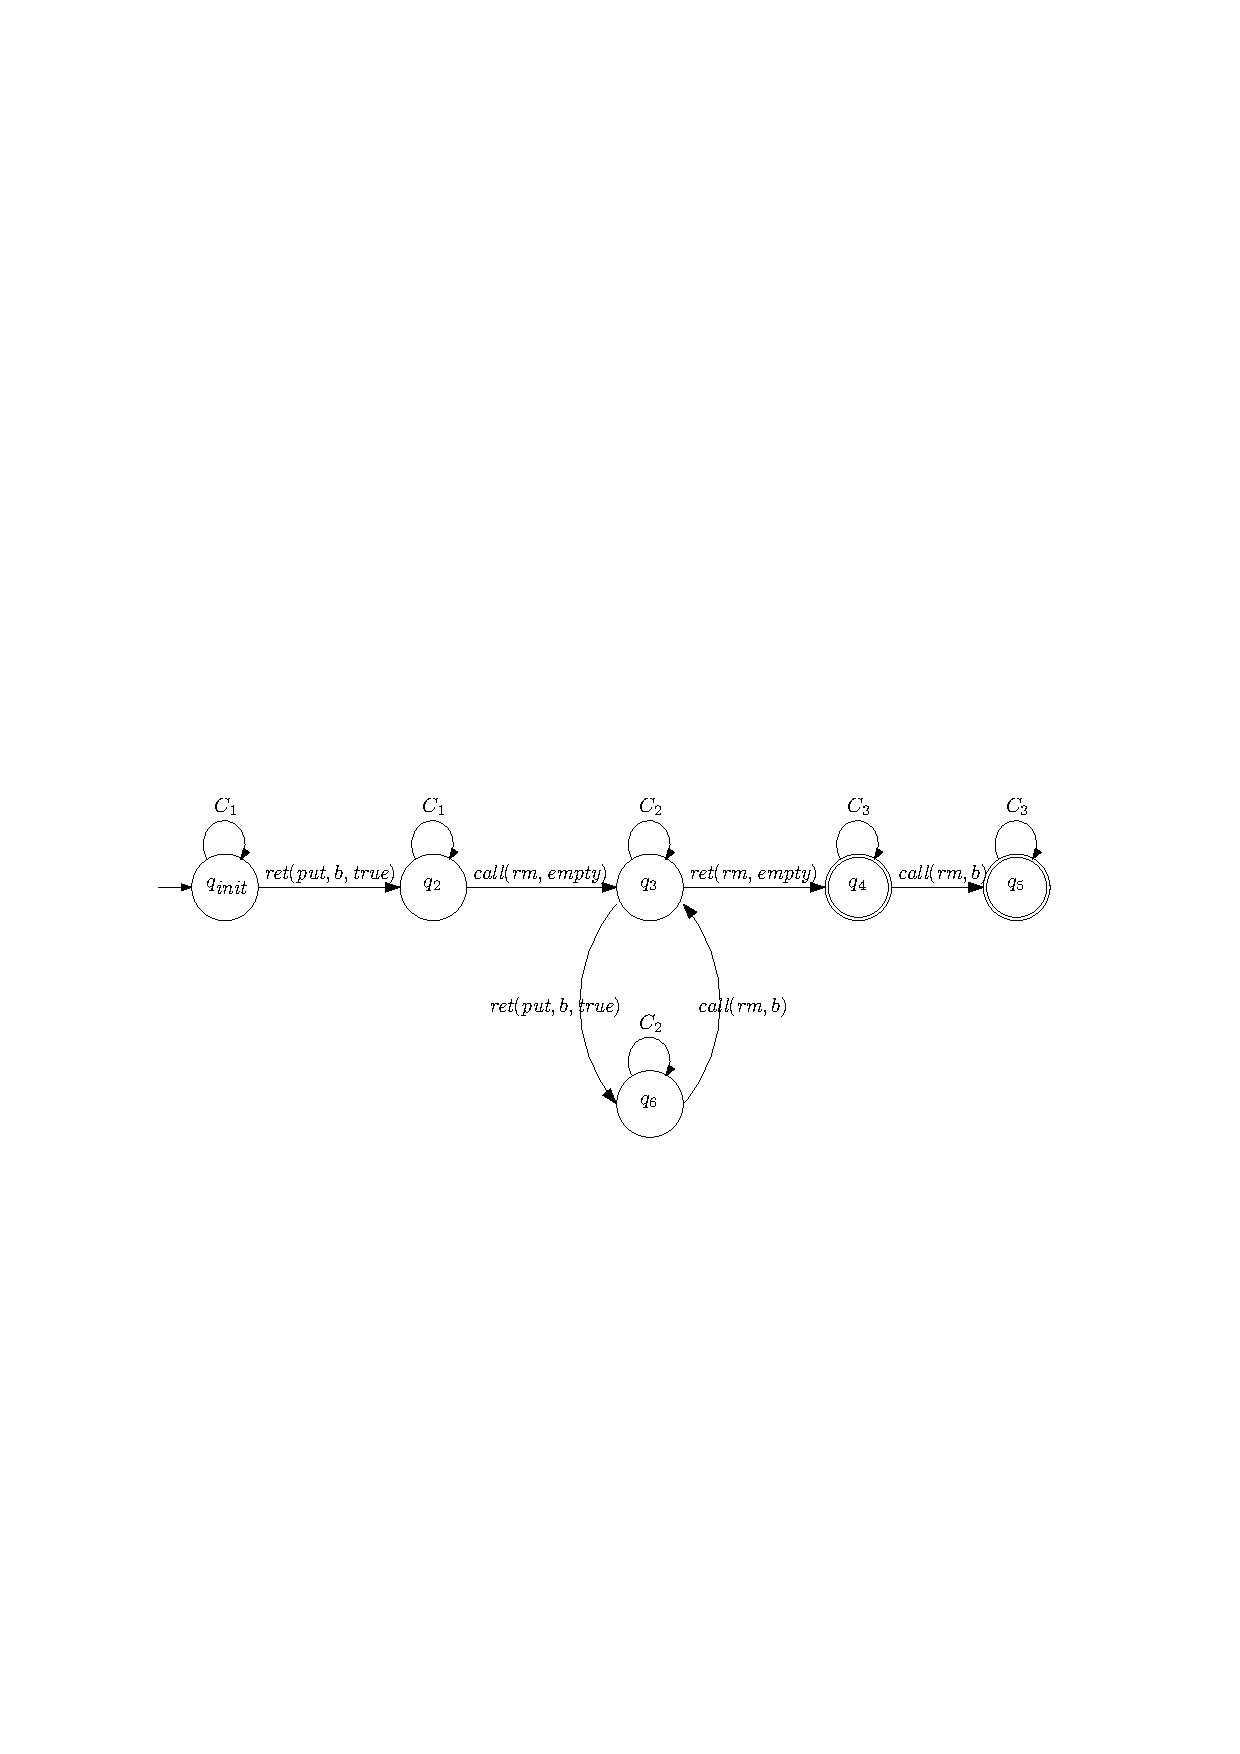
\includegraphics[width=0.8 \textwidth]{figures/PIC_AUTO_PQ3.pdf}
%\vspace{-10pt}
  \caption{Automaton $\mathcal{A}_{\textit{EPQ}}^3$}
  \label{fig:automata for PQ3}
\end{figure}

Given a data-differentiated execution $e$, we say that $o = \textit{rm}(\textit{empty})$ in $e$ is covered by items $d_1,\ldots,d_m$ in $h$, if

\begin{itemize}
\setlength{\itemsep}{0.5pt}
\item[-] $\textit{put}(d_m,\_)$ happens before $o$,

\item[-] For each $i < 1 \leq m$,$\textit{put}(d_{\textit{i-1}},\_)$ happens before $\textit{rm}(d_i)$,

\item[-] $o$ happens before $\textit{rm}(d_1)$, or $\textit{rm}(d_1)$ does not exists in $e$
\end{itemize}

According to the definition of left-right constraint for $o$, in a data-differentiated execution $e$, there is a cycle going through $o$, if and only if there exists items $d_1,\ldots,d_m$, such that $o$ is covered by $d_1,\ldots,d_m$.


\begin{restatable}{lemma}{EPQ3IsCoRegular}
\label{lemma:EPQ3 is co-regular}
$\textit{EPQ}_3$ is co-regular.
\end{restatable}

\begin {proof}

We need to prove that, given a data-independence implementation $\mathcal{I}$, $\mathcal{A}_{\textit{EPQ}}^3 \cap \mathcal{I} \neq \emptyset$ if and only if $\exists e \in \mathcal{I}_{\neq},e' \in \textit{proj}(e), last(e')=\textit{EPQ}_3 \wedge e$ does not linearizable w.r.t. $\textit{MS}(\textit{EPQ}_3)$.

By Lemma \ref{lemma:Lin Equals Constraint for EPQ3}, we need to prove the following fact:

\noindent {\bf $\textit{fact}_1$}: Given a data-independence implementation $\mathcal{I}$, $\mathcal{A}_{\textit{EPQ}}^3 \cap \mathcal{I} \neq \emptyset$ if and only if $\exists e \in \mathcal{I}_{\neq},e' \in \textit{proj}(e), last(e')=\textit{EPQ}_3$, $o = \textit{rm}(\textit{empty})$ is in $e'$, and $o$ is covered by some items $d_1,\ldots,d_m$ in $e'$.


\noindent The $\textit{only if}$ direction: Assume that $e_1 \in \mathcal{I}$ is accepted by $\mathcal{A}_{\textit{EPQ}}^3$. By data-independence, there exists data-differentiated execution $e_2 \in \mathcal{I}$ and a renaming function $r$, such that $e_1=r(e_2)$. Let $d_1,\ldots,d_m$ be the items in $e_2$ such that $r(d_i)=b$ for each $1 \leq i \leq m$. Let $e_3 = e_2 \vert_{ \{ o, d_1, \ldots, d_m \} }$. It is obvious that $e_3 \in \textit{proj}(e_2)$ and $\textit{last}(e_3) = \textit{EPQ}_3$. It is easy to see that $o$ is covered by $d_1,\ldots,d_m$.

\noindent The $\textit{if}$ direction: Assume that there exists such $e$, $e'$, $o$ and $d_1,\ldots,d_m$. Then, let $e_1$ be obtained from $e$ by renaming $d_1,\ldots,d_m$ into $b$ and renaming other items into $d$. By data-independence, $e_1 \in \mathcal{I}$. It is easy to see that $e_1$ is accepted by $\mathcal{A}_{\textit{EPQ}}^3$.

This completes the proof of this lemma. \qed
\end {proof}


\section{Proofs and Definitions in Section \ref{sec:relate other data structures with extended priority queue}}
\label{sec:appendix proof and definition in section relate other data structures with extended priority queue}


\subsection{Proofs and Definitions in Subsection \ref{subsec:relate multiSet with extended priority queue}}
\label{subsec:appendix proof and definition in section relate multiset with extended priority queue}

In this section, we use the notions of inductive rules, $\textit{last}$ of a sequential execution, step-by-step and co-regular in \cite{Bouajjani:2015}. Since they are quite similar to the corresponding notions of extended priority queues in Section \ref{sec:inductive rules of extended priority queue}, Section \ref{sec:step-by-step linearizability of extended priority queues} and Section \ref{sec:co-regular of extended priority queues}, we do not introduce their definitions here.

Let us first define three predicates:

\begin{itemize}
\setlength{\itemsep}{0.5pt}
\item[-] Given a sequential execution $l$ of multi-set, $\textit{noDE}(l)$ is satisfied when each method event of $l$ is not $\textit{delete}(\textit{empty})$.

\item[-] Given a sequential execution $l$ of multi-set, $\textit{matched-MS}(l)$ is satisfied, if (1) for each item $a \in \mathbb{D}$, if $\textit{insert}(a)$ is in $l$, then $\textit{delete}(a)$ is in $l$, and (2) for each item $a \in \mathbb{D}$, if $\textit{delete}(a)$ is in $l$, then $\textit{insert}(a)$ is in $l$.

\item[-] Given a sequential execution $l$ of multi-set, $l \in \textit{Insert}^*$ is satisfied when each method event of $l$ is a $\textit{insert}$ event.
\end{itemize}

Let $\textit{MSet}$ be the set of sequential executions $w$ which can be derived from the empty word by inductive rules of multi-set. $\textit{MSet}$ is defined by the following inductive rules:

\begin{itemize}
\setlength{\itemsep}{0.5pt}
\item[-] $\textit{MSet}_0 \equiv \epsilon \in \textit{MSet}$.

\item[-] $\textit{MSet}_1 \equiv (u \in \textit{MSet}) \wedge
(u \in \textit{Insert}^*)
\Rightarrow
(u \cdot \textit{insert}(\textit{itm}) \in \textit{MSet})$.

\item[-] $\textit{MSet}_2 \equiv
(u \cdot v \cdot w \in \textit{MSet}) \wedge
(\textit{noDE}(u \cdot v \cdot w))
\Rightarrow
(u \cdot \textit{insert}(\textit{itm}) \cdot v \cdot \textit{delete}(\textit{itm}) \cdot w \in \textit{MSet})$.

\item[-] $\textit{MSet}_3 \equiv
(u \cdot v \in \textit{MSet}) \wedge
(\textit{matched-MS}(u) )
\Rightarrow
(u \cdot \textit{delete}(\textit{empty}) \cdot v \in \textit{MSet})$.
\end{itemize}

Thus, given a sequential execution $e$, we define $\textit{last}(e)$ as the last possible rule to generate $e$ according to the rules of multi-set:

\begin{itemize}
\setlength{\itemsep}{0.5pt}
\item[-] If $e$ contains $\textit{delete}(\textit{empty})$, then $\textit{last}(e) = \textit{MS}_3$.

\item[-] Else, if $e$ contains $\textit{delete}$, then $\textit{last}(e) = \textit{MSet}_2$.

\item[-] Else, if $e$ contains only $\textit{insert}$, then $\textit{last}(e) = \textit{MSet}_1$.

\item[-] Else ($e = \epsilon$), $\textit{last}(e) = \textit{MSet}_0$.
\end{itemize}

The following three lemmas state that the rules for multi-set are step-by-step linearizability.

\begin{restatable}{lemma}{MS1isStepByStepLinearizability}
\label{lemma:MS1 is step-by-step linearizability}
If a differentiated concurrent execution $e$ is linearizable w.r.t. $\textit{MS}(\textit{MSet}_1)$ with witness $x$, then $e \setminus x \sqsubseteq \textit{MSet} \Rightarrow e \sqsubseteq \textit{MSet}$.
\end{restatable}

\begin {proof}
Let $h$ be the data-differentiated history of $e$, and $l$ be an sequential execution such that $h \sqsubseteq l$ and $l$ matches $\textit{MSet}_1$ with witness $x$. Let $h'=h \setminus x$ and assume that $h' \sqsubseteq l' \in \textit{MSet}$. Let $e_{\textit{lp}}$ be an execution with linearization points of $e$ and the linearization points is added according to $l'$. Or we can say, $e_{\textit{lp}}$ is generated from $e$ by instrumenting linearization points, and the projection of $e_{\textit{lp}}$ into method event is $l'$.

Let sequence $e'_{\textit{lp}}$ be generated from $e_{\textit{lp}}$ by adding $\textit{insert}(x)$ at an arbitrary time point between $\textit{cal}(\textit{insert},x)$ and $\textit{ret}(\textit{insert},x)$. Let $l''$ be the projection of $e'_{\textit{lp}}$ into method events.

It is easy to see that $h \sqsubseteq l''$. Since $l''$ is obtained from $l'$ by adding one $\textit{insert}(x)$, we can see that $l''$ contains only $\textit{insert}$, and then $l'' \in \textit{MSet}$. \qed
\end {proof}


\begin{restatable}{lemma}{MS2isStepByStepLinearizability}
\label{lemma:MS2 is step-by-step linearizability}
If a differentiated concurrent execution $e$ is linearizable w.r.t. $\textit{MS}(\textit{MSet}_2)$ with witness $x$, then $e \setminus x \sqsubseteq \textit{MSet} \Rightarrow e \sqsubseteq \textit{MSet}$.
\end{restatable}

\begin {proof}
Let $h$ be the data-differentiated history of $e$, and $l$ be an sequential execution such that $h \sqsubseteq l$ and $l$ matches $\textit{MSet}_1$ with witness $x$. Let $h'=h \setminus x$ and assume that $h' \sqsubseteq l' \in \textit{MSet}$. Let $e_{\textit{lp}}$ be an execution with linearization points of $e$ and the linearization points is added according to $l'$. Or we can say, $e_{\textit{lp}}$ is generated from $e$ by instrumenting linearization points, and the projection of $e_{\textit{lp}}$ into method event is $l'$.

It is easy to see that $\textit{delete}(x)$ does not happen before $\textit{insert}(x)$, and then $\textit{cal}(\textit{insert},x)$ is before $\textit{ret}(\textit{delete},x)$ in $e$. Let sequence $e'_{\textit{lp}}$ be generated from $e_{\textit{lp}}$ by adding $\textit{insert}(x)$ just after $\textit{cal}(\textit{insert},x)$ and adding $\textit{delete}(x)$ just before $\textit{ret}(\textit{delete},x)$. Let $l''$ be the projection of $e'_{\textit{lp}}$ into method events.

It is easy to see that $h \sqsubseteq l''$. Since (1) $l' \in \textit{MSet}$, (2) $l''$ is obtained from $l'$ by adding one $\textit{insert}(x)$ and one $\textit{delete}(x)$, while $\textit{insert}(x)$ is before $\textit{delete}(x)$ (3)and $l'$ does not contain $\textit{delete}(\textit{empty})$, we can see that $l'' \in \textit{MSet}$. \qed
\end {proof}


\begin{restatable}{lemma}{MS3isStepByStepLinearizability}
\label{lemma:MS3 is step-by-step linearizability}
If a differentiated concurrent execution $e$ is linearizable w.r.t. $\textit{MS}(\textit{MSet}_3)$ and $o$ is a $\textit{delete}(\textit{empty})$ event, then $e \setminus o \sqsubseteq \textit{MSet} \Rightarrow e \sqsubseteq \textit{MSet}$.
\end{restatable}

\begin {proof}
This Lemma can be similarly proved as Lemma \ref{lemma:EPQ3 is step-by-step linearizability}. \qed
\end {proof}

The following lemma states that $\textit{MSet}_1$ is always co-regular.

\begin{restatable}{lemma}{MS1IsAlwaysCoRegular}
\label{lemma:MS1 is always co-regular}
Given a differentiated execution $e$, if $\textit{last}(e) = \textit{MSet}_1$, then $e \sqsubseteq \textit{MS}(\textit{MSet}_1)$.
\end{restatable}

\begin {proof}
Since $\textit{last}(e) = \textit{MSet}_1$, there are only $\textit{insert}$ in $e$. Then no matter how we locate linearization points of operations of $e$, we can always obtain a sequence in $\textit{MS}(\textit{MSet}_1)$. This completes the proof of this lemma. \qed
\end {proof}

The following lemma shows how to detect violation to $\textit{MS}(\textit{MSet}_2)$.

\begin{restatable}{lemma}{ReduceMS2intoOneValue}
\label{lemma:reduce MS2 into one value}
Given a differentiated execution $e$, there exists some $e' \in \textit{proj}(e)$, such that $\textit{last}(e') = \textit{MSet}_2$ and $e'$ doe not linearizable w.r.t $\textit{MS}(\textit{MSet}_2)$, if and only if one of the following case holds for some $x \in \mathbb{D}$.
\begin{itemize}
\setlength{\itemsep}{0.5pt}
\item[-] $\textit{delete}(x)$ is in $e$ while $\textit{insert}(x)$ is not in $e$.

\item[-] there is more than one $\textit{delete}(x)$ in $e$ and one $\textit{insert}(x)$ in $e$.

\item[-] $\textit{delete}(x) <_{\textit{hb}} \textit{insert}(x)$ in $e$.
\end{itemize}
\end{restatable}

\begin {proof}

The $\textit{only if}$ is obvious and omitted here.

To prove the $\textit{if}$ direction, we prove its contrapositive. Assume that for each item $x$ of $e$, the following conditions are satisfied:

\begin{itemize}
\setlength{\itemsep}{0.5pt}
\item[-] If $\textit{delete}(x)$ is in $e$, then $\textit{insert}(x)$ is also in $e$.

\item[-] There is at most $\textit{delete}(x)$ in $e$.

\item[-] $\textit{delete}(x)$ does not happen before $\textit{insert}(x)$.
\end{itemize}

Assume by contradiction that there exists some $e' \in \textit{proj}(e)$, such that $\textit{last}(e') = \textit{MSet}_2$ and $e'$ doe not linearizable w.r.t $\textit{MS}(\textit{MSet}_2)$. Since $\textit{last}(e') = \textit{MSet}_2$, there exists $\textit{delete}$ in $e$. Let this $\textit{delete}$ operation be $\textit{delete}(a)$. By assumption, we know that in $e$ there exists one $\textit{insert}(a)$ and one $\textit{delete}(a)$, and $\textit{delete}(a)$ does not happen before $\textit{insert}(a)$. Then we know that $\textit{cal}(\textit{insert},x)$ is before $\textit{ret}(\textit{delete},x)$.

Let $e_{\textit{lp}}$ be generated from $e$ by (1) put the linearization of $\textit{insert}(x)$ just after $\textit{cal}(\textit{insert},x)$, (2) put the linearization of $\textit{delete}(x)$ just before $\textit{ret}(\textit{insert},x)$, and (3) for other operations, put its linearization point at an arbitrary between its call and return actions. Let $l'$ be the projection of $e_{\textit{lp}}$ into method events. It is obvious that $h \sqsubseteq l'$. According to our construction of $e_{\textit{lp}}$, we can see that in $l'$, $\textit{insert}(x)$ is before $\textit{delete}(x)$. Therefore, we can see that $l' \in \textit{MS}(\textit{MSet}_2)$, which contradicts our assumption. This completes the proof of the $\textit{id}$ direction. \qed
\end {proof}

According to Lemma \ref{lemma:reduce MS2 into one value}, to check violation to $\textit{MS}(\textit{MSet}_2)$, we need to consider three cases for some $b \in \mathbb{D}$: (1) there is $\textit{delete}(b)$ but there is not $\textit{insert}(x)$, (2) there is more than one $\textit{delete}(b)$ and one $\textit{insert}(b)$ in $e$, and (3) $\textit{delete}(b) <_{\textit{hb}} \textit{insert}(b)$.

For each such case, we construct a witness automata. We generate witness automata $\mathcal{A}_{\textit{MS}}^1$ for the first case, and it is shown in \figurename~\ref{fig:automata 1 for MS-2 in appendix}. Here $c_1 = \textit{cal}(\textit{insert},a),\textit{ret}(\textit{insert},a)$, $\textit{cal}(\textit{delete},a),\textit{ret}(\textit{delete},a),
\textit{cal}(\textit{delete},\textit{empty}),\textit{ret}(\textit{delete},\textit{empty})$, $c_2 = c_1 + \textit{cal}(\textit{delete},b) + \textit{ret}(\textit{delete},b)$.


\begin{figure}[htbp]
  \centering
  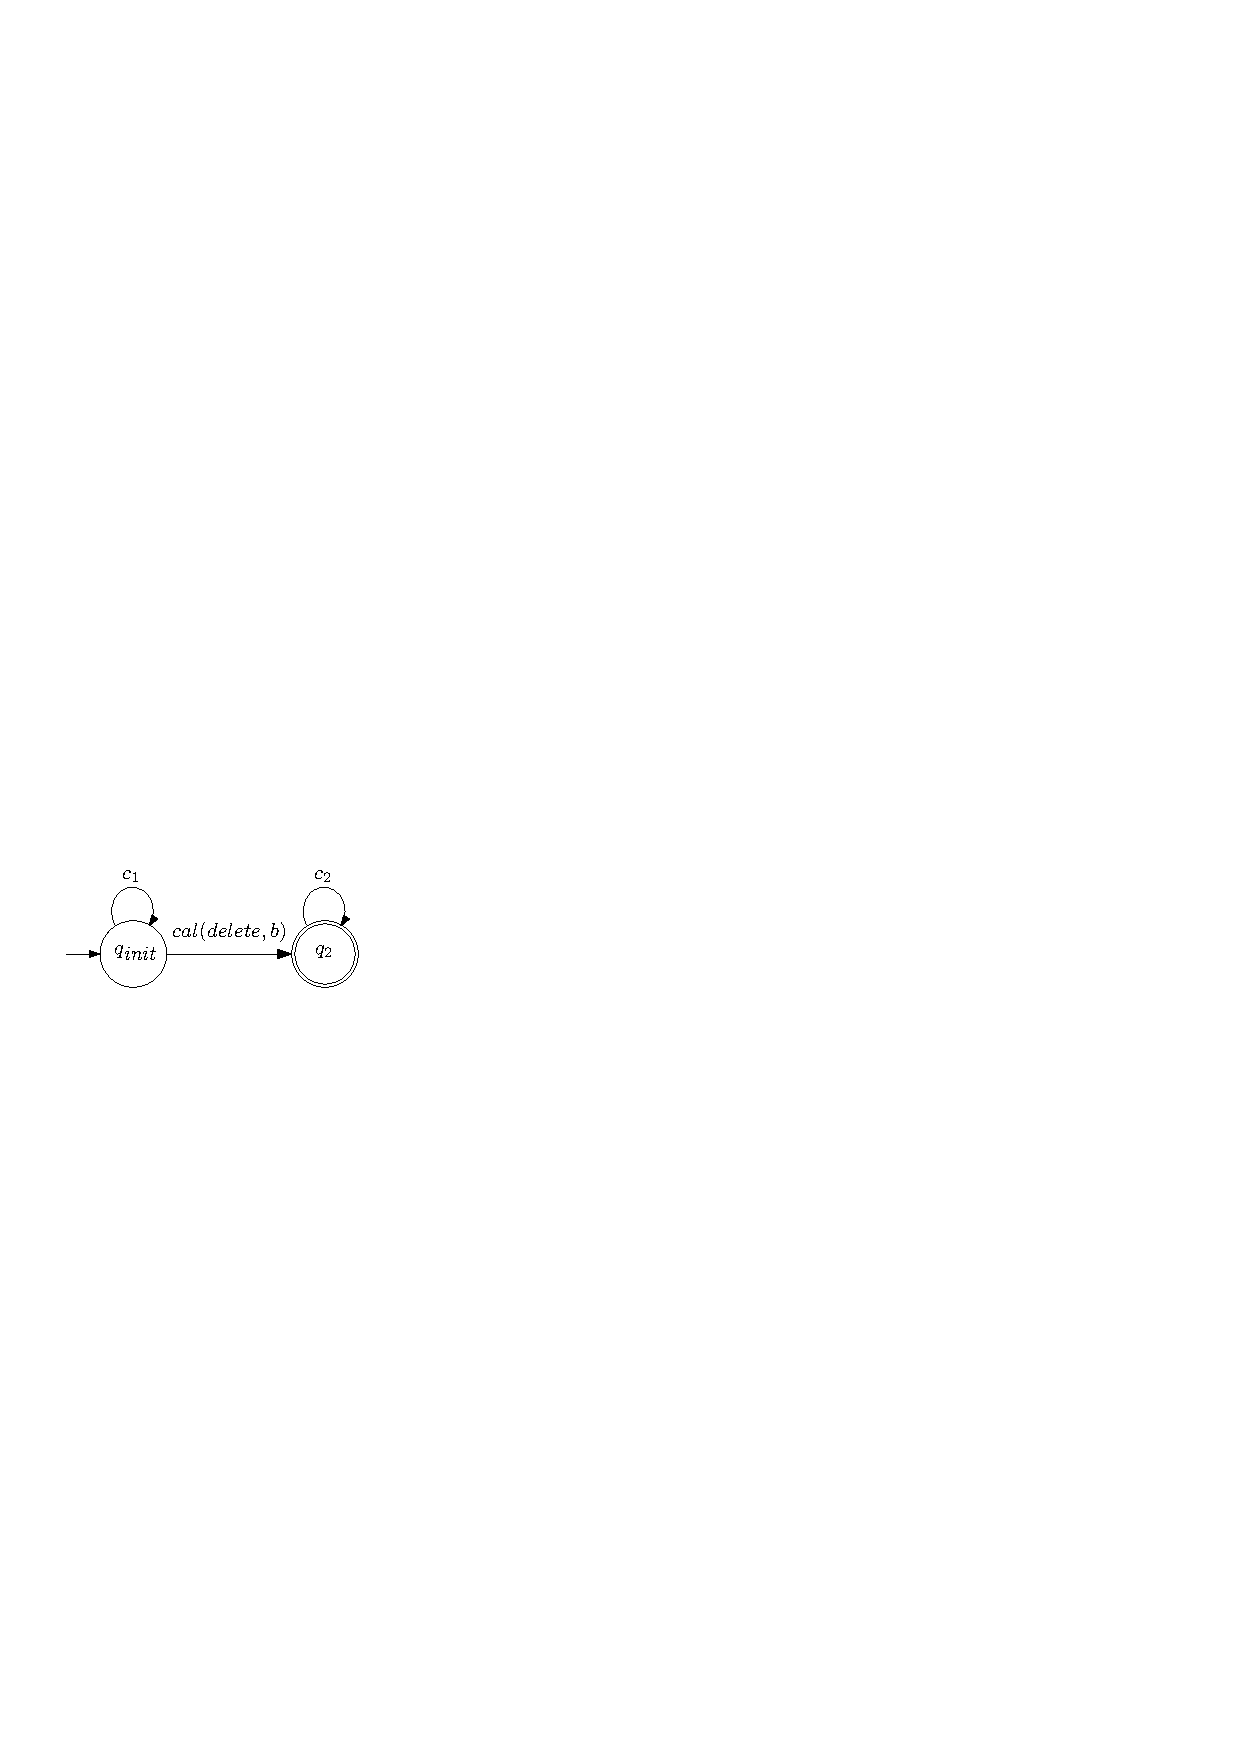
\includegraphics[width=0.3 \textwidth]{figures/PIC_AUTO_MS_1.pdf}
%\vspace{-10pt}
  \caption{Automaton $\mathcal{A}_{\textit{MS}}^1$}
  \label{fig:automata 1 for MS-2 in appendix}
\end{figure}


We generate witness automata $\mathcal{A}_{\textit{MS}}^2$ for the second case, and it is shown in \figurename~\ref{fig:automata 2 for MS-2 in appendix}. Here $c_1 = \textit{cal}(\textit{insert},a),\textit{ret}(\textit{insert},a), \textit{cal}(\textit{delete},a),\textit{ret}(\textit{delete},a),\textit{cal}(\textit{delete},\textit{empty})$, $\textit{ret}(\textit{delete},\textit{empty})$, $c_2 = c_1 + \textit{ret}(\textit{insert},b)$, $c_3 = c_2 + \textit{ret}(\textit{delete},b)$, $c_4 = c_3 + \textit{cal}(\textit{delete},b)$, $c_5 = c_1 + \textit{ret}(\textit{delete},b)$, $c_6 = c_5 + \textit{cal}(\textit{delete},b)$.

\begin{figure}[htbp]
  \centering
  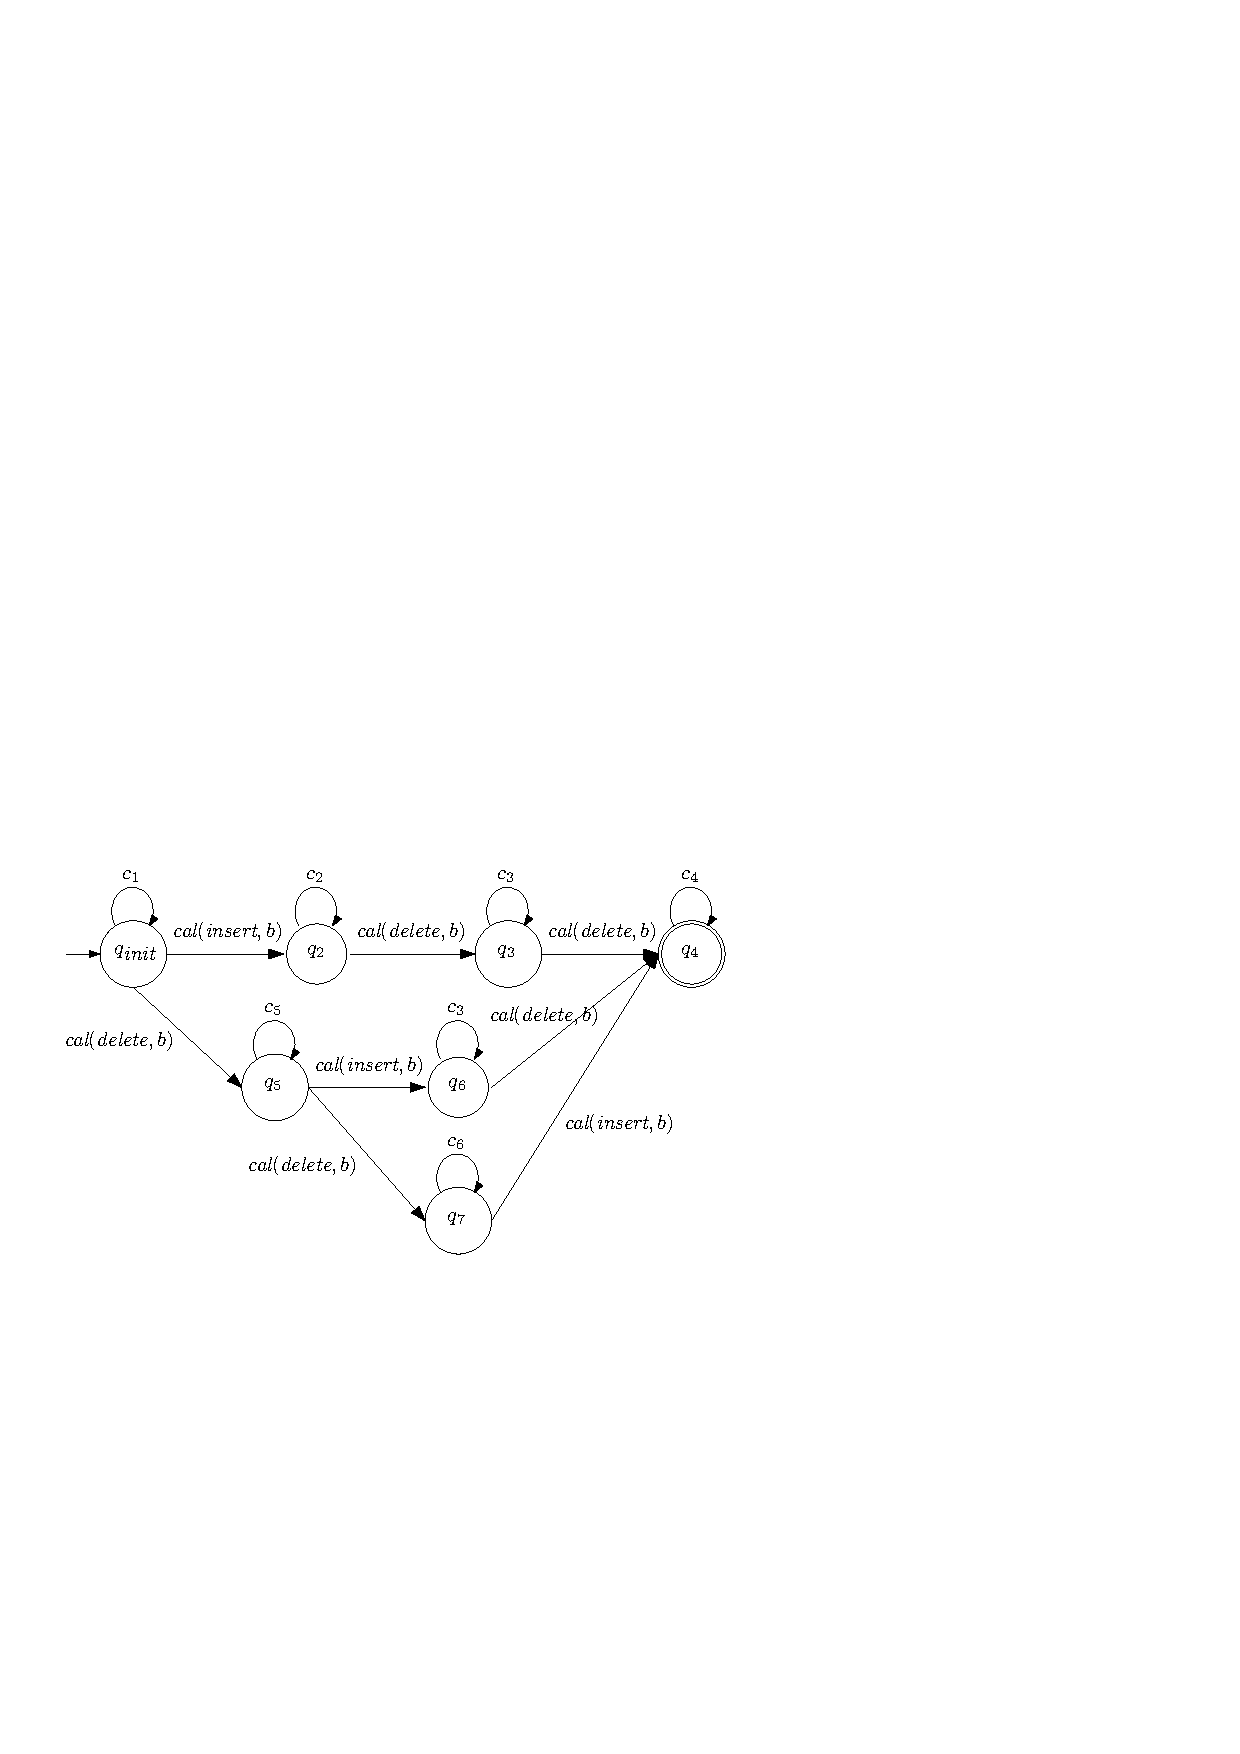
\includegraphics[width=0.7 \textwidth]{figures/PIC_AUTO_MS_2.pdf}
%\vspace{-10pt}
  \caption{Automaton $\mathcal{A}_{\textit{MS}}^2$}
  \label{fig:automata 2 for MS-2 in appendix}
\end{figure}


We generate witness automata $\mathcal{A}_{\textit{MS}}^3$ for the third case, and it is shown in \figurename~\ref{fig:automata 3 for MS-2 in appendix}. Here $c_1 = \textit{cal}(\textit{insert},a)$, $\textit{ret}(\textit{insert},a)$, $\textit{cal}(\textit{delete},a)$, $\textit{ret}(\textit{delete},a),\textit{cal}(\textit{delete},b)$, $\textit{cal}($ $\textit{delete},\textit{empty}),\textit{ret}(\textit{delete},\textit{empty})$, $c_2 = c_1 + \textit{ret}(\textit{delete},b)$, $c_3 = c_2 + \textit{ret}(\textit{insert},b)$.

\begin{figure}[htbp]
  \centering
  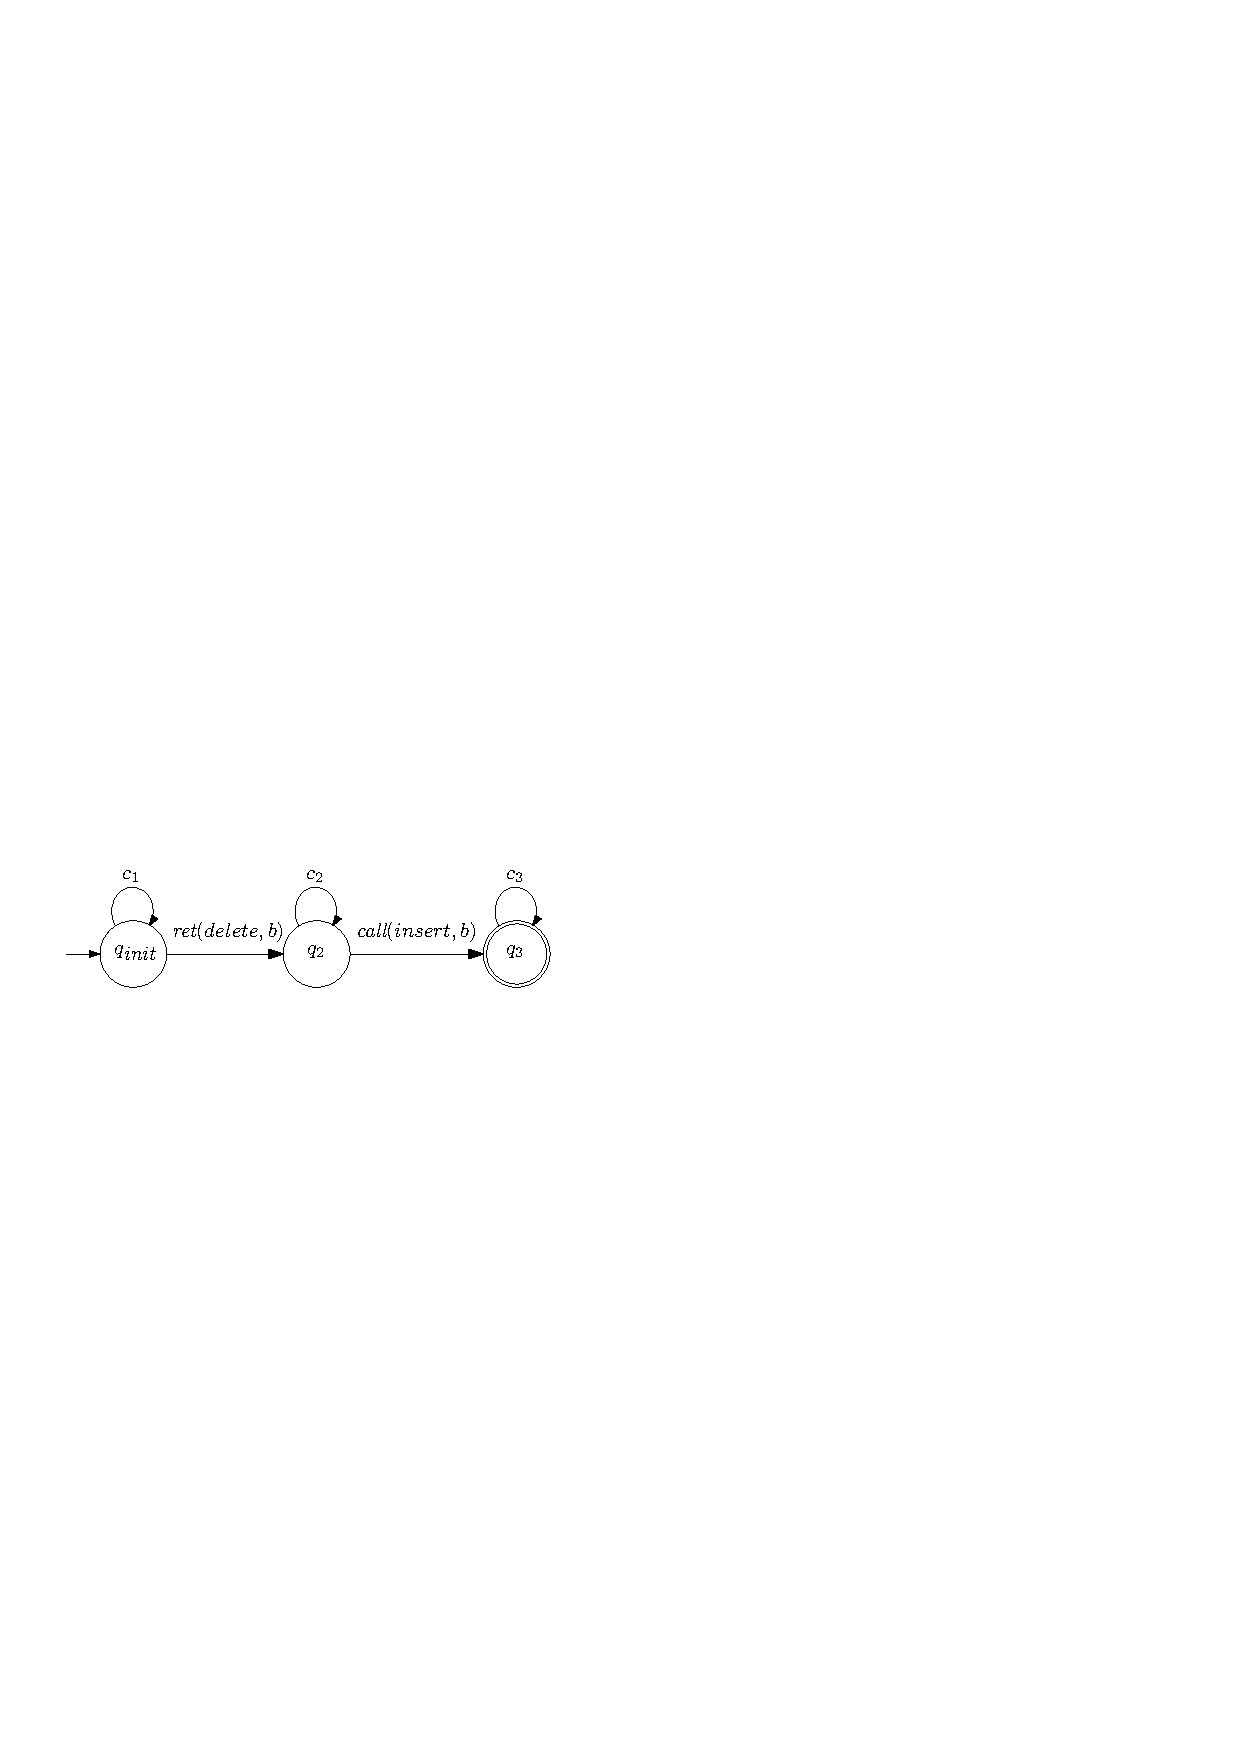
\includegraphics[width=0.6 \textwidth]{figures/PIC_AUTO_MS_3.pdf}
%\vspace{-10pt}
  \caption{Automaton $\mathcal{A}_{\textit{MS}}^3$}
  \label{fig:automata 3 for MS-2 in appendix}
\end{figure}


Let $\textit{Auts}_{\textit{2-ms}} = \{ \mathcal{A}_{\textit{MS}}^1, \mathcal{A}_{\textit{MS}}^2, \mathcal{A}_{\textit{MS}}^3 \}$. The following lemma states that $\textit{MS}_2$ is co-regular.


\begin{restatable}{lemma}{MS2IsCoRegular}
\label{lemma:MS2 is co-regular}
$\textit{MSet}_2$ is co-regular.
\end{restatable}

\begin {proof}

According to \cite{Bouajjani:2015}, we need to prove that, given a independence implementation $\mathcal{I}$, $\textit{Auts}_{\textit{2-ms}} \cap \mathcal{I} \neq \emptyset$, if and only if $\exists e \in \mathcal{I}_{\neq},$ $e' \in \textit{proj}(e),$ $\textit{last}(e') = \textit{MSet}_2 \wedge e'$ does not linearizable w.r.t. $\textit{MS}(\textit{MSet}_2)$.

By Lemma \ref{lemma:reduce MS2 into one value}, we need to prove the following fact:

\noindent {\bf $\textit{fact}_1$}: given a independence implementation $\mathcal{I}$, $\textit{Auts}_{\textit{2-ms}} \cap \mathcal{I} \neq \emptyset$, if and only if $\exists e \in \mathcal{I}_{\neq}$, and one of the following case holds for some $x \in \mathbb{D}$.
\begin{itemize}
\setlength{\itemsep}{0.5pt}
\item[-] $\textit{delete}(x)$ is in $e$ while $\textit{insert}(x)$ is not in $e$.

\item[-] there is more than one $\textit{delete}(x)$ in $e$ and one $\textit{insert}(x)$ in $e$.

\item[-] $\textit{delete}(x) <_{\textit{hb}} \textit{insert}(x)$ in $e$.
\end{itemize}

\noindent The $\textit{only if}$ direction: Assume that $e_1 \in \mathcal{I}$ is accepted by some witness automata in $\textit{Auts}_{\textit{1-eq}}$. By data-independence, there exists data-differentiated execution $e_2 \in \mathcal{I}$ and a renaming function $r$, such that $e_1=r(e_2)$. Since $e_1$ is accepted by some witness automata in  $\textit{Auts}_{\textit{1-eq}}$, let $y$ be the item that are renamed into $b$ by $r$. Then it is not hard to see that $y$ satisfies one of three conditions in $e_2$.

\noindent The $\textit{if}$ direction: Assume that there exists such $e \in \mathcal{I}_{\neq}$ and $x$. Let renaming function $r$ maps $x$ into $b$ and all other items into $a$. By data-independence, we can see that $r(e) \in \mathcal{I}$. Then it is easy to see that $r(e)$ is accepted by some automaton in $\textit{Auts}_{\textit{2-ms}}$. \qed
\end {proof}

Similar to Lemma \ref{lemma:EPQ3 is co-regular}, we can prove that $\textit{MSet}_3$ is co-regular, as stated by the following lemma.

\begin{restatable}{lemma}{MSet3IsCoRegular}
\label{lemma:MSet3 is co-regular}
$\textit{MSet}_3$ is co-regular.
\end{restatable}

Similar as witness automata for $\textit{EPQ}_3$, we have witness automata $\mathcal{A}_{\textit{MS}}^4$ for $\textit{MSet}_3$, which is shown in \figurename~\ref{fig:automata 4 for MS-3 in appendix}. In \figurename~\ref{fig:automata 4 for MS-3 in appendix}, let $c = \textit{cal}(\textit{insert},d),\textit{ret}(\textit{insert},d), \textit{cal}(\textit{delete},d)$, $\textit{ret}(\textit{delete},d),\textit{cal}(\textit{delete},\textit{empty}),\textit{ret}(\textit{delete},\textit{empty})$, $c_1 = c + \textit{cal}(\textit{insert},b)$, $c_2 = c_1 + \textit{ret}(\textit{delete},b)$, and $c_3 = c + \textit{ret}(\textit{delete},b)$.

\begin{figure}[htbp]
  \centering
  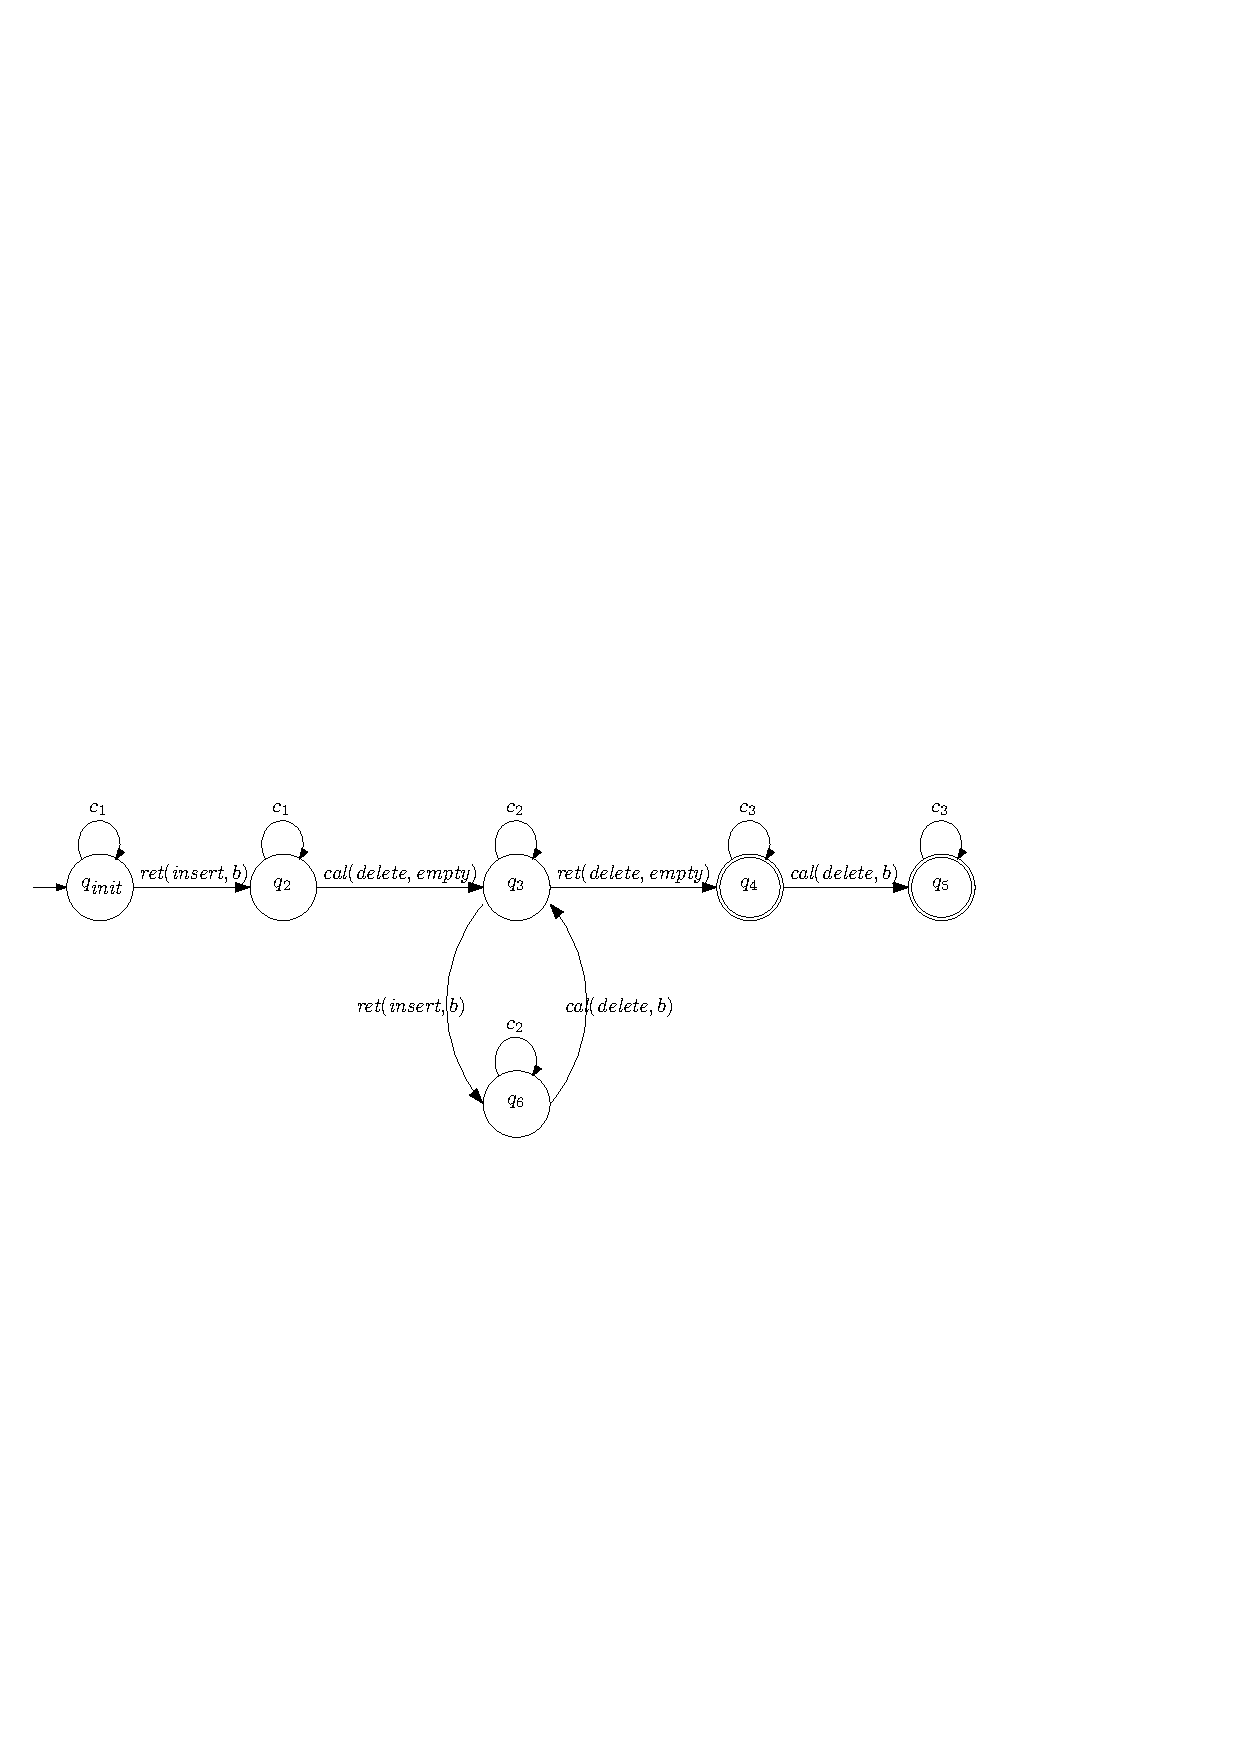
\includegraphics[width=0.8 \textwidth]{figures/PIC_AUTO_MS_4.pdf}
%\vspace{-10pt}
  \caption{Automaton $\mathcal{A}_{\textit{MS}}^4$}
  \label{fig:automata 4 for MS-3 in appendix}
\end{figure}

The following lemma shows that our transformation from multi-set into extended priority queue is correct.

\RelateMultiSetwithEPQ*

\begin {proof}

For the $\textit{only if}$ direction, given an execution $e_m \in \mathcal{I}_m$ of multi-set, such that $e_m$ is accepted by some automaton in $\textit{Auts}_{\textit{MS}}$. If $e_m$ is accepted by $\mathcal{A}_{\textit{MS}}^1$, $\mathcal{A}_{\textit{MS}}^2$, $\mathcal{A}_{\textit{MS}}^3$ or $\mathcal{A}_{\textit{MS}}^4$, then it is easy to see that $\textit{MStoEPQ}(e_m)$ is accepted by $\mathcal{A}_{\textit{SinPri}}^2$, $\mathcal{A}_{\textit{SinPri}}^3$, $\mathcal{A}_{\textit{SinPri}}^1$ or $\mathcal{A}_{\textit{EPQ}}^3$, respectively.

For the $\textit{if}$ direction, given an execution $e_{\textit{epq}}$ of extended priority queue, such that $e_{\textit{epq}} = \textit{MStoEPQ}(e_m)$ for some $e_m$ of multi-set, and $e_{\textit{epq}}$ is accepted by some automaton in $\textit{Auts}_{\textit{EPQ}}$.

According to definition of $\textit{MStoEPQ}$, we can see that (1) in $e_{\textit{epq}}$ there does not exist two items with comparable priorities, and (2) in $e_{\textit{epq}}$, there does not exists two items with a same priority. Therefore, the witness automata for $\textit{EPQ}_1$ and the witness automaton $\mathcal{A}_{\textit{SinPri}}^4$ can be safely ignored. Then, if $e_{\textit{epq}}$ is accepted by $\mathcal{A}_{\textit{SinPri}}^1$, $\mathcal{A}_{\textit{SinPri}}^2$, $\mathcal{A}_{\textit{SinPri}}^3$ or $\mathcal{A}_{\textit{EPQ}}^3$, then it is easy to see that $e_m$ is accepted by $\mathcal{A}_{\textit{MS}}^3$, $\mathcal{A}_{\textit{MS}}^1$, $\mathcal{A}_{\textit{MS}}^2$ and $\mathcal{A}_{\textit{MS}}^4$, respectively. \qed
\end {proof}



\subsection{Proofs and Definitions in Subsection \ref{subsec:relate stack with extended priority queue}}
\label{subsec:appendix proof and definition in section relate stack with extended priority queue}






